%-------------------------------------------------------------------------------
% ATLAS paper format
%-------------------------------------------------------------------------------
\pdfoutput=1
% The \pdfoutput command is needed by arXiv/JHEP/JINST to ensure use of pdflatex.
% It should be included in the first 5 lines of the file.
%-------------------------------------------------------------------------------
% Specify where ATLAS LaTeX style files can be found.
\newcommand*{\ATLASLATEXPATH}{latex/}
% Use this variant if the files are in a central location, e.g. $HOME/texmf.
% \newcommand*{\ATLASLATEXPATH}{}
%-------------------------------------------------------------------------------
%\documentclass[PAPER,USenglish,coverpage,texlive=2016, english]{\ATLASLATEXPATH atlasdoc}
\documentclass[PAPER, american,coverpage,texlive=2016, english]{\ATLASLATEXPATH atlasdoc}
% \documentclass[PAPER,USenglish]{\ATLASLATEXPATH atlasdoc}

% The language of the document must be set: usually UKenglish or USenglish.
% british and american also work!
% Commonly used options:
%  texlive=YYYY          Specify TeX Live version (2013 is default).
%  atlasstyle=true|false Use ATLAS style for document (default).
%  coverpage             Create ATLAS draft cover page for collaboration circulation.
%                        See atlas-draft-cover.tex for a list of variables that should be defined.
%  cernpreprint          Create front page for a CERN preprint.
%                        See atlas-preprint-cover.tex for a list of variables that should be defined.
%  PAPER                 The document is an ATLAS paper (draft).
%  CONF                  The document is a CONF note (draft).
%  PUB                   The document is a PUB note (draft).
%  BOOK                  The document is of book form, like an LOI or TDR (draft)
%  txfonts=true|false    Use txfonts rather than the default newtx - needed for arXiv submission.
%  paper=a4|letter       Set paper size to A4 (default) or letter.
\newcommand*{\VH}{\ensuremath{VH}\xspace}
\newcommand*{\ttH}{\ensuremath{t\bar{t}H}\xspace}
\newcommand*{\muH}{\ensuremath{\mu_{H}}\xspace}
\newcommand*{\muVBF}{\ensuremath{\mu_{\text{VBF}}}\xspace}



%-------------------------------------------------------------------------------
% Extra packages:
\usepackage[subfigure]{\ATLASLATEXPATH atlaspackage}
% Commonly used options:
%  biblatex=true|false   Use biblatex (default) or bibtex for the bibliography.
%  backend=biber         Use the biber backend rather than bibtex.
%  subfigure|subfig|subcaption  to use one of these packages for figures in figures.
%  minimal               Minimal set of packages.
%  default               Standard set of packages.
%  full                  Full set of packages.
%-------------------------------------------------------------------------------
% Style file with biblatex options for ATLAS documents.
\usepackage{\ATLASLATEXPATH atlasbiblatex}
% \usepackage{subcaption}

% Package for creating list of authors and contributors to the analysis.
\usepackage{\ATLASLATEXPATH atlascontribute}

% Useful macros
\usepackage[process]{\ATLASLATEXPATH atlasphysics}
% See doc/atlas_physics.pdf for a list of the defined symbols.
% Default options are:
%   true:  journal, misc, particle, unit, xref
%   false: BSM, heppparticle, hepprocess, hion, jetetmiss, math, process, other, texmf
% See the package for details on the options.

% Files with references for use with biblatex.
% Note that biber gives an error if it finds empty bib files.
\addbibresource{VBFPaper2016.bib}
\addbibresource{bibtex/bib/ATLAS.bib}
\addbibresource{bibtex/bib/CMS.bib}
\addbibresource{bibtex/bib/ConfNotes.bib}
\addbibresource{bibtex/bib/PubNotes.bib}

% Paths for figures - do not forget the / at the end of the directory name.
\graphicspath{{logos/}{figures/}{figures/aux/}}

% Add you own definitions here (file VBFPaper2016-defs.sty).
\usepackage{VBFPaper2016-defs}

\usepackage{multirow}
\usepackage{seqsplit}



%-------------------------------------------------------------------------------
% Generic document information
%-------------------------------------------------------------------------------

% Title, abstract and document
%-------------------------------------------------------------------------------
% This file contains the title, author and abstract.
% It also contains all relevant document numbers used by the different cover pages.
%-------------------------------------------------------------------------------

% Title
%\AtlasTitle{Search for the Higgs Boson Decaying to Bottom Quark Pairs Produced in Association with Jets and Photons}
\AtlasTitle{Search for Higgs bosons produced via vector-boson fusion and decaying into bottom quark pairs in $\sqrt{s} = \SI{13}{\TeV}$ $pp$ collisions with the ATLAS detector}

% Author - this does not work with revtex (add it after \begin{document})
\author{The ATLAS Collaboration}

% Authors and list of contributors to the analysis
% \AtlasAuthorContributor also adds the name to the author list
% Include package latex/atlascontribute to use this
% Use authblk package if there are multiple authors, which is included by latex/atlascontribute
% \usepackage{authblk}
% Use the following 3 lines to have all institutes on one line
% \makeatletter
% \renewcommand\AB@affilsepx{, \protect\Affilfont}
% \makeatother
% \renewcommand\Authands{, } % avoid ``. and'' for last author
% \renewcommand\Affilfont{\itshape\small} % affiliation formatting
%\AtlasAuthorContributor{First AtlasAuthorContributor}{a}{Author's contribution.}
% \AtlasAuthorContributor{Second AtlasAuthorContributor}{b}{Author's contribution.}
% \AtlasAuthorContributor{Third AtlasAuthorContributor}{a}{Author's contribution.}
% \AtlasContributor{Fourth AtlasContributor}{Contribution to the analysis.}
% \author[a]{First Author}
% \author[a]{Second Author}
% \author[b]{Third Author}
% \affil[a]{University of California, Santa Cruz}
% \affil[b]{Stanford University}
% \affil[c]{SLAC National Accelerator Laboratory}
% \affil[d]{}
% \affil[e]{}
% \affil[f]{}

% If a special author list should be indicated via a link use the following code:
% Include the two lines below if you do not use atlasstyle:
% \usepackage[marginal,hang]{footmisc}
% \setlength{\footnotemargin}{0.5em}
% Use the following lines in all cases:
% \usepackage{authblk}
% \author{The ATLAS Collaboration%
% \thanks{The full author list can be found at:\newline
%   \url{https://atlas.web.cern.ch/Atlas/PUBNOTES/ATL-PHYS-PUB-2016-007/authorlist.pdf}}
% }

% Draft version:
% Should be 1.0 for the first circulation, and 2.0 for the second circulation.
% If given, adds draft version on front page, a 'DRAFT' box on top of each other page, 
% and line numbers.
% Comment or remove in final version.
\AtlasVersion{2.4}

% ATLAS reference code, to help ATLAS members to locate the paper
\AtlasRefCode{HIGG-2016-30}

% ATLAS note number. Can be an COM, INT, PUB or CONF note
% \AtlasNote{ATLAS-CONF-2016-XXX}
% \AtlasNote{ATL-PHYS-PUB-2016-XXX}
%\AtlasNote{ATL-COM-PHYS-2017-671}
\AtlasNote{HIGG-2016-30}

% CERN preprint number
% \PreprintIdNumber{CERN-PH-2018-XX}

% ATLAS date - arXiv submission; usually filled in by the Physics Office
% \AtlasDate{\today}

% ATLAS heading - heading at top of title page. Set for TDR etc.
% \AtlasHeading{ATLAS ABC TDR}

% arXiv identifier
% \arXivId{14XX.YYYY}

% HepData record
% \HepDataRecord{ZZZZZZZZ}

% Submission journal and final reference
 \AtlasJournal{Phys.\ Rev.\ D.}
% \AtlasJournalRef{\PLB 789 (2014) 123}
% \AtlasDOI{}

% Abstract - % directly after { is important for correct indentation
\AtlasAbstract{%
A search for the $b\bar b$ decay of the Standard Model Higgs boson produced through vector-boson fusion is presented.
Three mutually exclusive channels are considered: two all-hadronic channels and a photon-associated channel. 
Results are reported from the analysis of up to \SI{30.6}{\ifb} of $pp$ data at $\sqrt{s} = \SI{13}{\TeV}$ collected with the ATLAS detector at the LHC.  The measured signal strength relative to the Standard Model prediction from the combined analysis is $2.5^{+1.4}_{-1.3}$  for inclusive Higgs boson production and $3.0^{+1.7}_{-1.6}$ for vector-boson fusion production only.
}

%-------------------------------------------------------------------------------
% The following information is needed for the cover page. The commands are only defined
% if you use the coverpage option in atlasdoc or use the atlascover package
%-------------------------------------------------------------------------------

% List of supporting notes  (leave as null \AtlasCoverSupportingNote{} if you want to skip this option)
\AtlasCoverSupportingNote{Hadronic channels}{https://cds.cern.ch/record/2235643}
\AtlasCoverSupportingNote{Photon channel}{https://cds.cern.ch/record/2234295}

% Comment deadline
\AtlasCoverCommentsDeadline{30 May 2018}

% Analysis team members - contact editors should no longer be specified
% as there is a generic email list name for the editors
\AtlasCoverAnalysisTeam{Zihao Jiang, Matthew Klein, Fabian Kukuck, Zhijun Liang, Bo Liu, Javier Llorente Merino, Jason Nielsen, Fabrizio Parodi, Jacob Pasner, Peyton Rose, Francesco Rubbo, Carlo Schiavi, Ariel Schwartzman, Liaoshan Shi, Lauren Tompkins, Carlo Varni, Song-Ming Wang}

% Editorial Board Members - indicate the Chair by a (chair) after his/her name
% Give either all members at once (then they appear on one line), or separately
\AtlasCoverEdBoardMember{Heather Gray~(chair), G\"{o}tz Gaycken, Richard Batley}

% Editors egroup
\AtlasCoverEgroupEditors{atlas-HIGG-2016-30-editors@cern.ch}

% EdBoard egroup
\AtlasCoverEgroupEdBoard{atlas-HIGG-2016-30-editorial-board@cern.ch}


% Author and title for the PDF file
\hypersetup{pdftitle={Search for Higgs Bosons Produced via Weak Boson Fusion and Decaying to Bottom Quark Pairs},pdfauthor={The ATLAS Collaboration}}

%-------------------------------------------------------------------------------
% Content
%-------------------------------------------------------------------------------
\begin{document}

\maketitle

%-------------------------------------------------------------------------------
\section{Introduction}
\label{sec:intro}
%-------------------------------------------------------------------------------
\input{content/introduction}
%-------------------------------------------------------------------------------
\section{ATLAS detector}
\label{sec:detector}

%-------------------------------------------------------------------------------
The name ATLAS is short for \textit{A Toroidal LHC Apparatus}. It is a multi-purpose particle detector which is designed primarily to detect and measure particles coming out of proton-proton collisions. The detector is located 100 meters underground at the LHC point one so that it is shielded from cosmic rays and weighs about 7000 tons. The ATLAS detector has a forward-backward symmetric cylindrical geometry with radius of 25 meters and length 44 meters. Over three thousand collaborators work at the ATLAS experiment. By design and for cross validation purpose, the ATLAS detector is very similar in regard of its functionality to its counterpart the CMS (Compact Muon Solenoid) detector at LHC point five. 

The collaboration uses a right-handed coordinate system as the convention. The beam pipe which penetrates through the detector is the $z$-axis of the coordinate system, while the origin of which is the beam interaction point (IP) also the center of the detector. The $x$-axis points from the origin of the detector towards the LHC ring center while $y$ axis points upward to the ground. Cylindrical coordinate is used in addition to the Cartesian coordinate described above. The $x-y$ plane parameterized by ($r,\phi$) where $r$ is the radius inside the plane and $\phi$ is the azimuthal angle around the beam. A polar angle $\theta$ is also defined with respect to the beam. The particle pseudorapidity defined as $\eta = -\ln \tan(\theta/2)$ is more commonly used than the polar angle as the difference between two massless particles' pseudorapidity is Lorentz invariant. The measure in the angular plane is defined as $\Delta R = \sqrt{\Delta \phi^2+\Delta \eta^2}$.

The ATLAS detector has approximately $4\pi$ coverage in solid angle. It contains many sub-systems as shown in Fig.\ref{fig:detector-atlas} which are used to measure different properties of the particles as well as distinguish different types of them. The major sub-components are the inner tracking detector, electromagnetic and hadronic calorimeters, and a muon spectrometer. There is also a dedicated data acquisition system to read out, filter and save the massive amount of data collected by these systems. The inner-most part of the detector is the inner detector,more details to be found in Sec.\ref{sec:detector-id}, primarily used to measure the charged-particle trajectories. A superconducting solenoid provides 2T magnetic field pointing in the $z$ direction can bend the charged-particles which will leave energy deposits on the layers of the inner detector, first few of which are silicon pixel layers followed by semiconductor microstrips (SCT) and then a transition radiation tracker (TRT). Most of the particles produced from the collisions end their journey in the calorimeter system, see Sec.\ref{sec:detector-calo}. The combination of electromagnetic lead/liquid-argon (LAr) calorimeter and the hadronic calorimeter built with steel/scintillator tiles measures the energies of particles. Only neutrinos and muons typically go beyond the calorimeters. Neutrinos hardly interact with materials and escape the detector while muons then enters the muon spectrometer with superconducting toroids providing 4T magentic field as will be described in Sec.\ref{sec:detector-mu}. The data coming out of the detector goes through a trigger system (Sec.\ref{sec:detector-trigger}) in order not to swap the disk. First level of filtering is done with level one trigger (L1) implemented in hardware. Another level of software trigger then accepts events at a even smaller rate. 


\begin{figure}[htpb!]
\begin{center}
  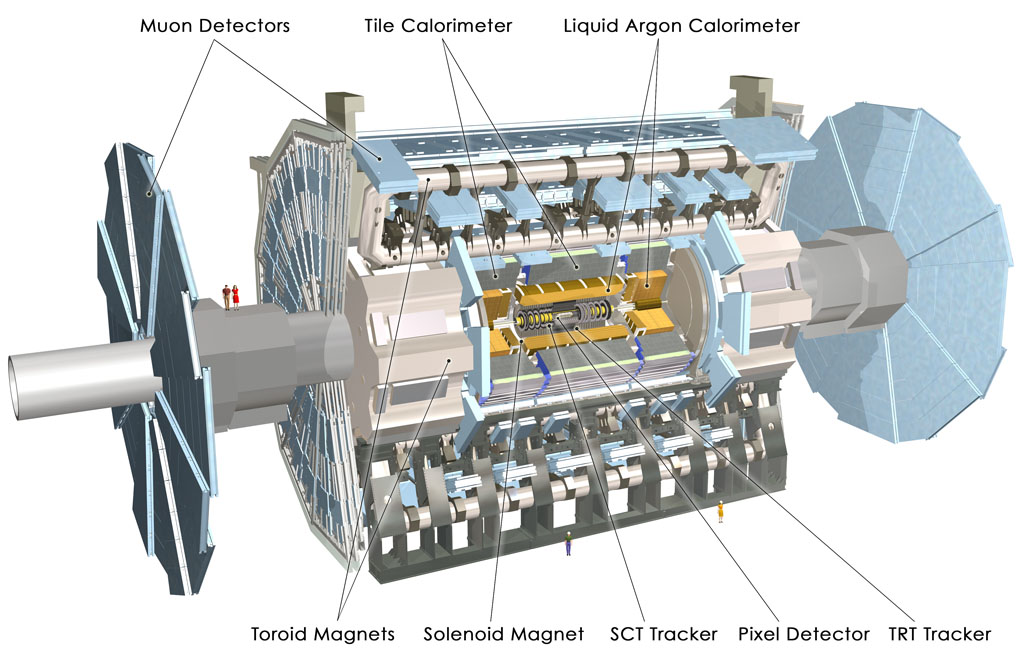
\includegraphics[width=0.85\linewidth]{figures/detector/ATLAS_Silver_White_MK}
\caption{View of the ATLAS detector and its sub-systems}
\label{fig:detector-atlas}
\end{center}
\end{figure}



%-------------------------------------------------------------------------------
\section{Signal and background simulation}
\label{sec:simulation}
%-------------------------------------------------------------------------------
The generic dijet events which include abundant quark and gluon jets generated with \textsc{Pythia} 8~\cite{Pythia,Pythia8} using the A14 tune~\cite{ATL-PHYS-PUB-2014-021}, the NNPDF2.3~\cite{Ball:2014uwa} PDF set, and processed with a full simulation of the ATLAS detector~\cite{Agostinelli:2002hh,Aad:2010ah} is used for this study.  Additional samples generated with \textsc{Sherpa} 2.1.1 (CT10 PDF~\cite{Gao:2013xoa}) and \textsc{Herwig++} 2.7.1 (UE-EE5 tune~\cite{Seymour:2013qka} and CTEQ6L1 PDF~\cite{Stump:2003yu}) are used to quantify the model dependence. Both \textsc{Pythia} 8 and \textsc{Herwig++} is interfaced with \textsc{EvtGen} v1.2.0~\cite{Lange:2001uf} for heavy flavor decays.

As quarks and gluons carry color charge and jets are color neutral, 
there is some ambiguity in the labeling of jets in simulation as quark or gluon.
In this study, jets in simulation are 
labeled based on the highest-energy parton emerging from the hard-scatter collision within the jet catchment area~\cite{jetareas}, 
just as was used and studied in previous studies~\cite{ATL-PHYS-PUB-2017-009}.
Only jets labeled as gluon or light quark (i.e. excluding bottom and top quark) are considered.

%-------------------------------------------------------------------------------
\section{Datasets and object reconstruction}
\label{sec:objects}
%-------------------------------------------------------------------------------

\input{content/object}
%-------------------------------------------------------------------------------
\section{Event selection}
\label{sec:selection}
%-------------------------------------------------------------------------------

\input{content/eventselection}


%-------------------------------------------------------------------------------
\section{Multivariate analysis}
\label{sec:mva}
%-------------------------------------------------------------------------------
\input{content/mva}

%-------------------------------------------------------------------------------
\section{Background and signal modeling}
\label{sec:backgrounds}
%-------------------------------------------------------------------------------
\input{content/background}


%-------------------------------------------------------------------------------
\section{Systematic uncertainties}
\label{sec:uncertainties}
%-------------------------------------------------------------------------------
\input{content/systematic}


%-------------------------------------------------------------------------------
\section{Fits for Higgs boson production}
\label{sec:results}
%-------------------------------------------------------------------------------
The VBF \Hbb analysis unblinding proceeds in two steps. First, overall strategy is validated with a fit to the $Z$ contribution in a sideband only fit while the Higgs mass window is kept unblinded, shown in Section~\ref{sec:vbf-zunblind}.  Then a simultaneous fit to the signal, correlated over all signal regions, and the $Z$ signal, uncorrelated across signal regions, is done over the entire mass region, as described in~\ref{sec:vbf-higgsunblind}. As an alternative interpretation of this analysis the $\mu_{VBF}$ strength is extracted by only allowing $VBF$ events to float in the fit and fixing all other Higgs processes, i.e. ggF, ttH and VH, to Standard Model expectation, as described in~\ref{sec:vbf-higgsunblindvbf}. The combination of inclusive $VBF$ and $VBF+\gamma$ results are presented in~\ref{sec:vbf-higgscomb}.


\subsection{Unblinding of \zjets{} in mass sidebands}
\label{sec:vbf-zunblind}

The fit strategy is first validated in data with a closure obtained in \zjets{} mass sideband fit. We performed a side-band only fit to extract the \zjets{} contribution independently in all regions. The fitted \zjets{} strengths are summarized in Table~\ref{tab:zsidebandfit}, presented with with all experimental and statistical uncertainties.   Note that we have no BDT shape uncertainties on the \zjets{} MC so cannot draw any conclusions from the compatibility of $\mu_Z$ with 1 in the different BDT regions. The effective $\mu_{Z}^{\rm eff}$ of all regions combined is defined as
\begin{equation}
\label{eqn:zsig}
\mu_{Z}^{\rm eff} = \sum \mu_{Z,i}\frac{n_{Z,i}}{\sum n_{Z,i}} 
\end{equation}
where $n_{Z,i}$ is the number of $Z$ events in region $i$, and $\mu_{Z,i}$ is the measured $\mu_Z$ in region $i$.  $\mu_{Z}^{\rm eff}$ is measured to be $1.0\pm 0.4$ in the sideband only fit with a compatibility of $\chi^2/nodf = 5.5/6=0.9$ ($\chi^2$ probability of 48\%).


\begin{table}[htbp]
\centering
\caption{Floating Z normalization parameters in data sideband fit including all systematic uncertainties.}
\label{tab:zsidebandfit}
\begin{tabular}{|l|c|c|}
\hline
Channel      & $\mu_{Z}$   & $\chi^2/ndof$ \\ \hline
2 cen SR I   & 2.6 $\pm$1.3  & 1.1          \\ \hline
2 cen SR II  & 0.4$\pm$0.8  & 0.7          \\ \hline
4 cen SR I   & 2.2$\pm$2.0  & 0.8          \\ \hline
4 cen SR II  & 2.0$\pm$1.9  & 0.9          \\ \hline
4 cen SR III & 1.9$\pm$0.6  & 0.9          \\ \hline
4 cen SR IV  & 0.6$\pm$0.6  & 0.9          \\ \hline
\end{tabular}
\end{table}



%\begin{figure}[htbp]
%  \centering
% 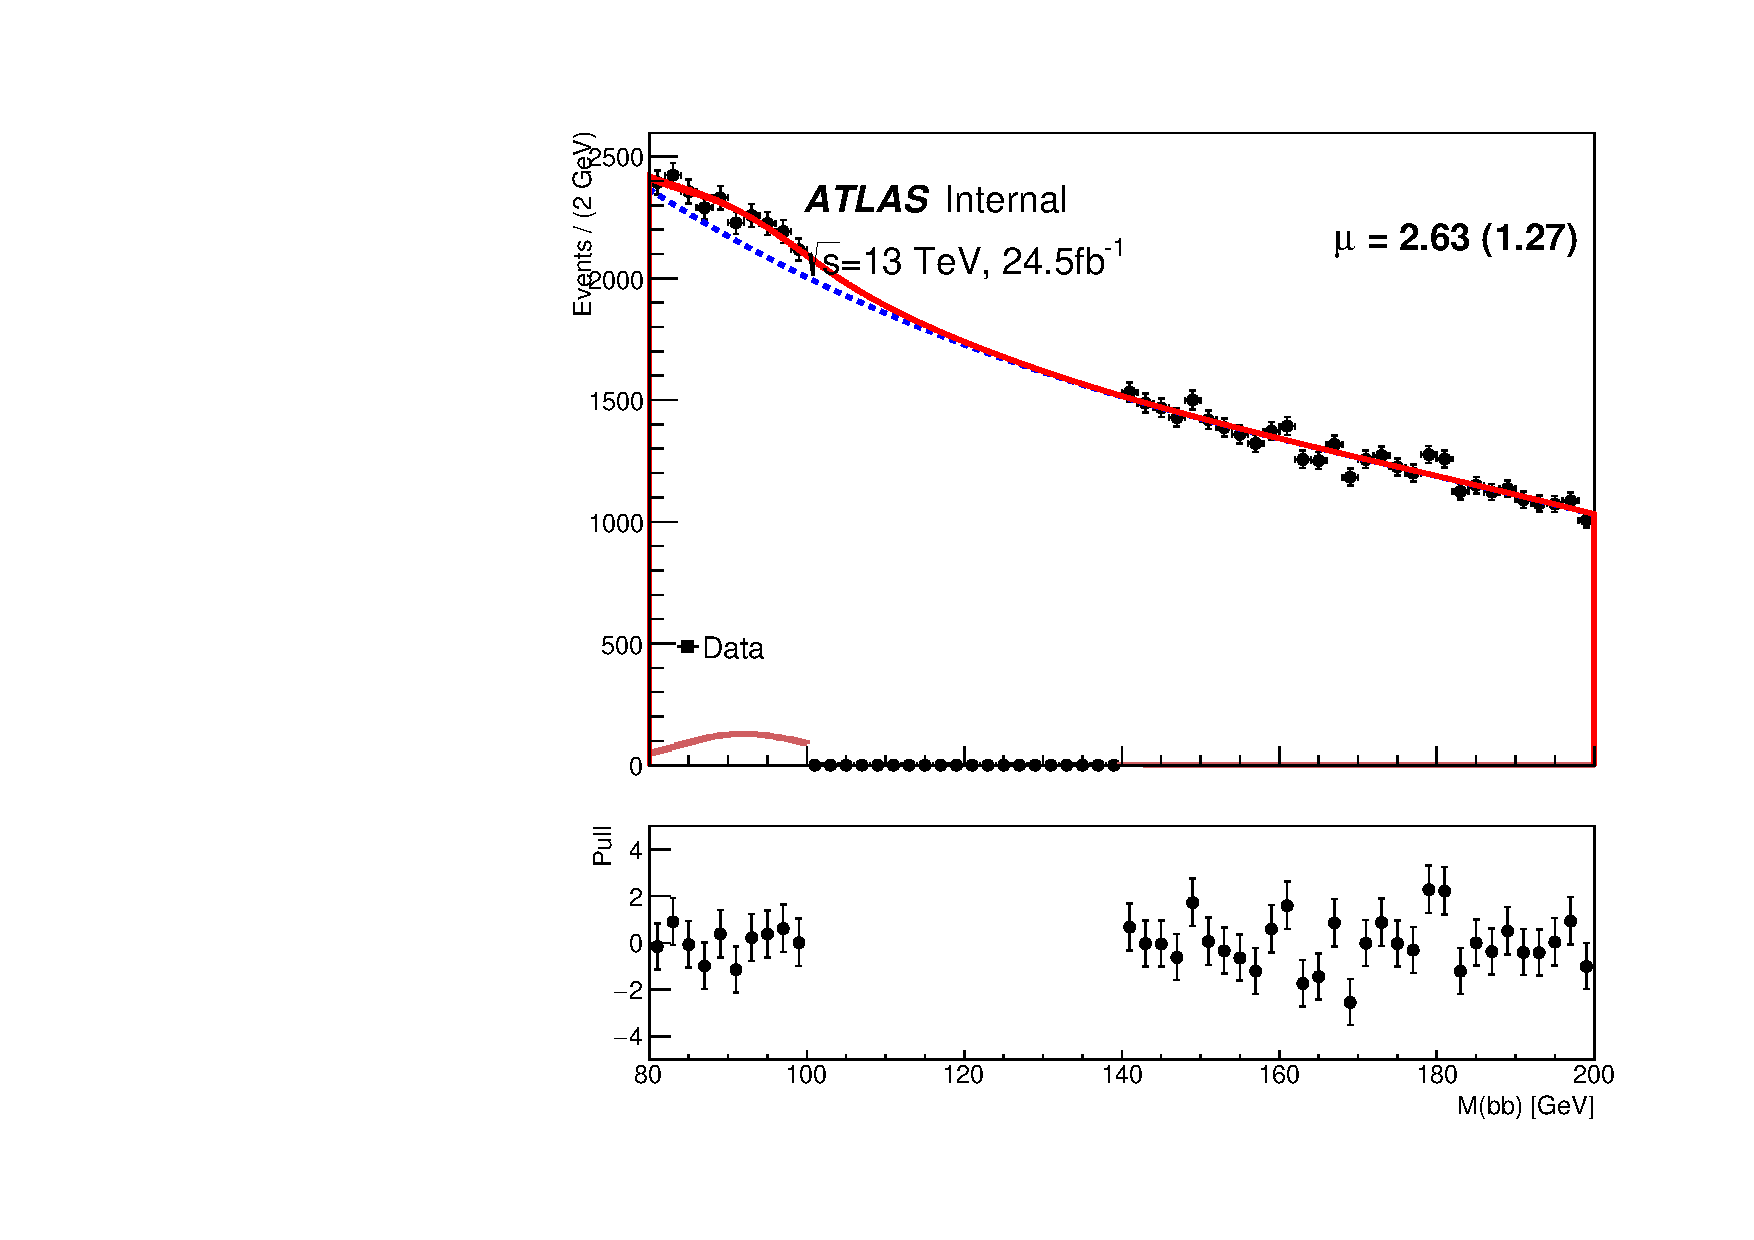
\includegraphics[width=0.24\textwidth]{figures/VBF/zunblind_testVBF_ICHEP_2cen_SRI.pdf}
% 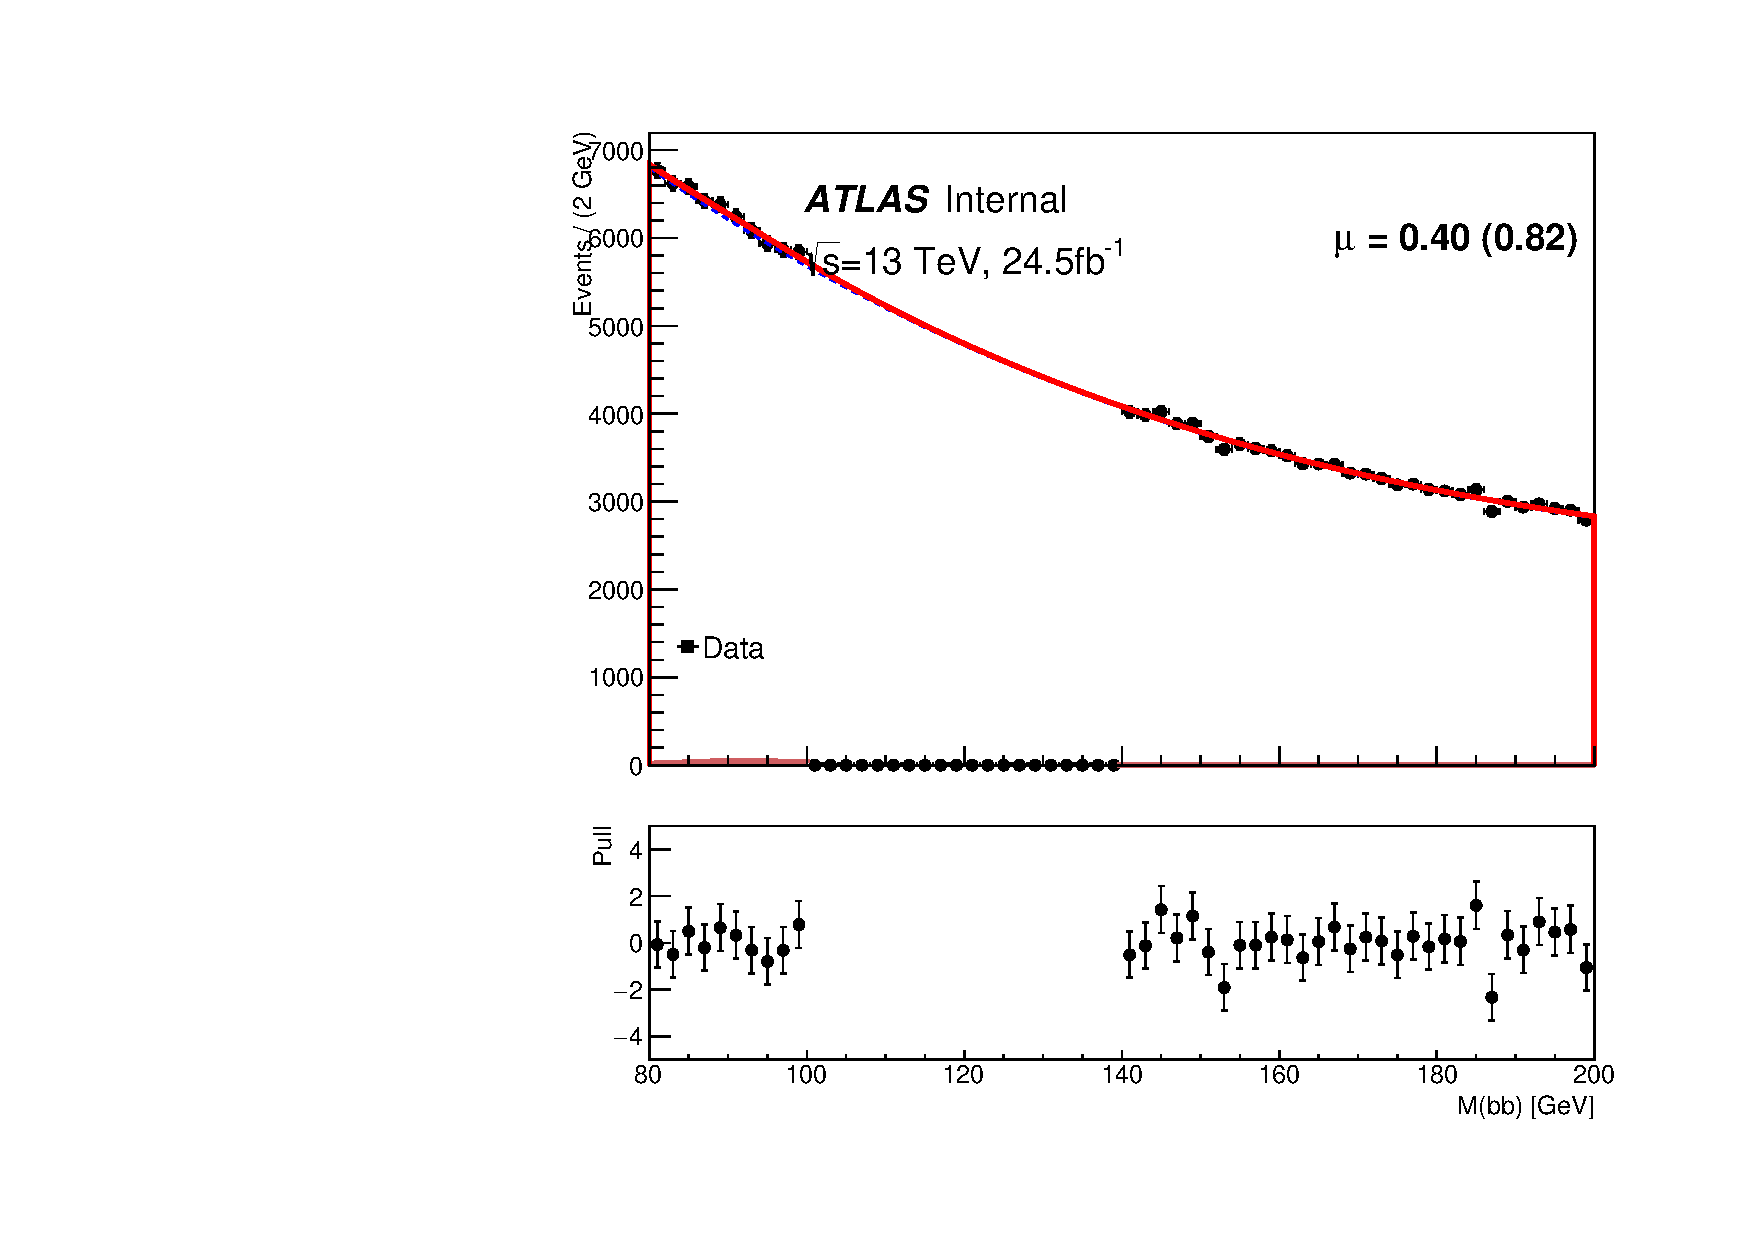
\includegraphics[width=0.24\textwidth]{figures/VBF/zunblind_testVBF_ICHEP_2cen_SRII.pdf}\\
% 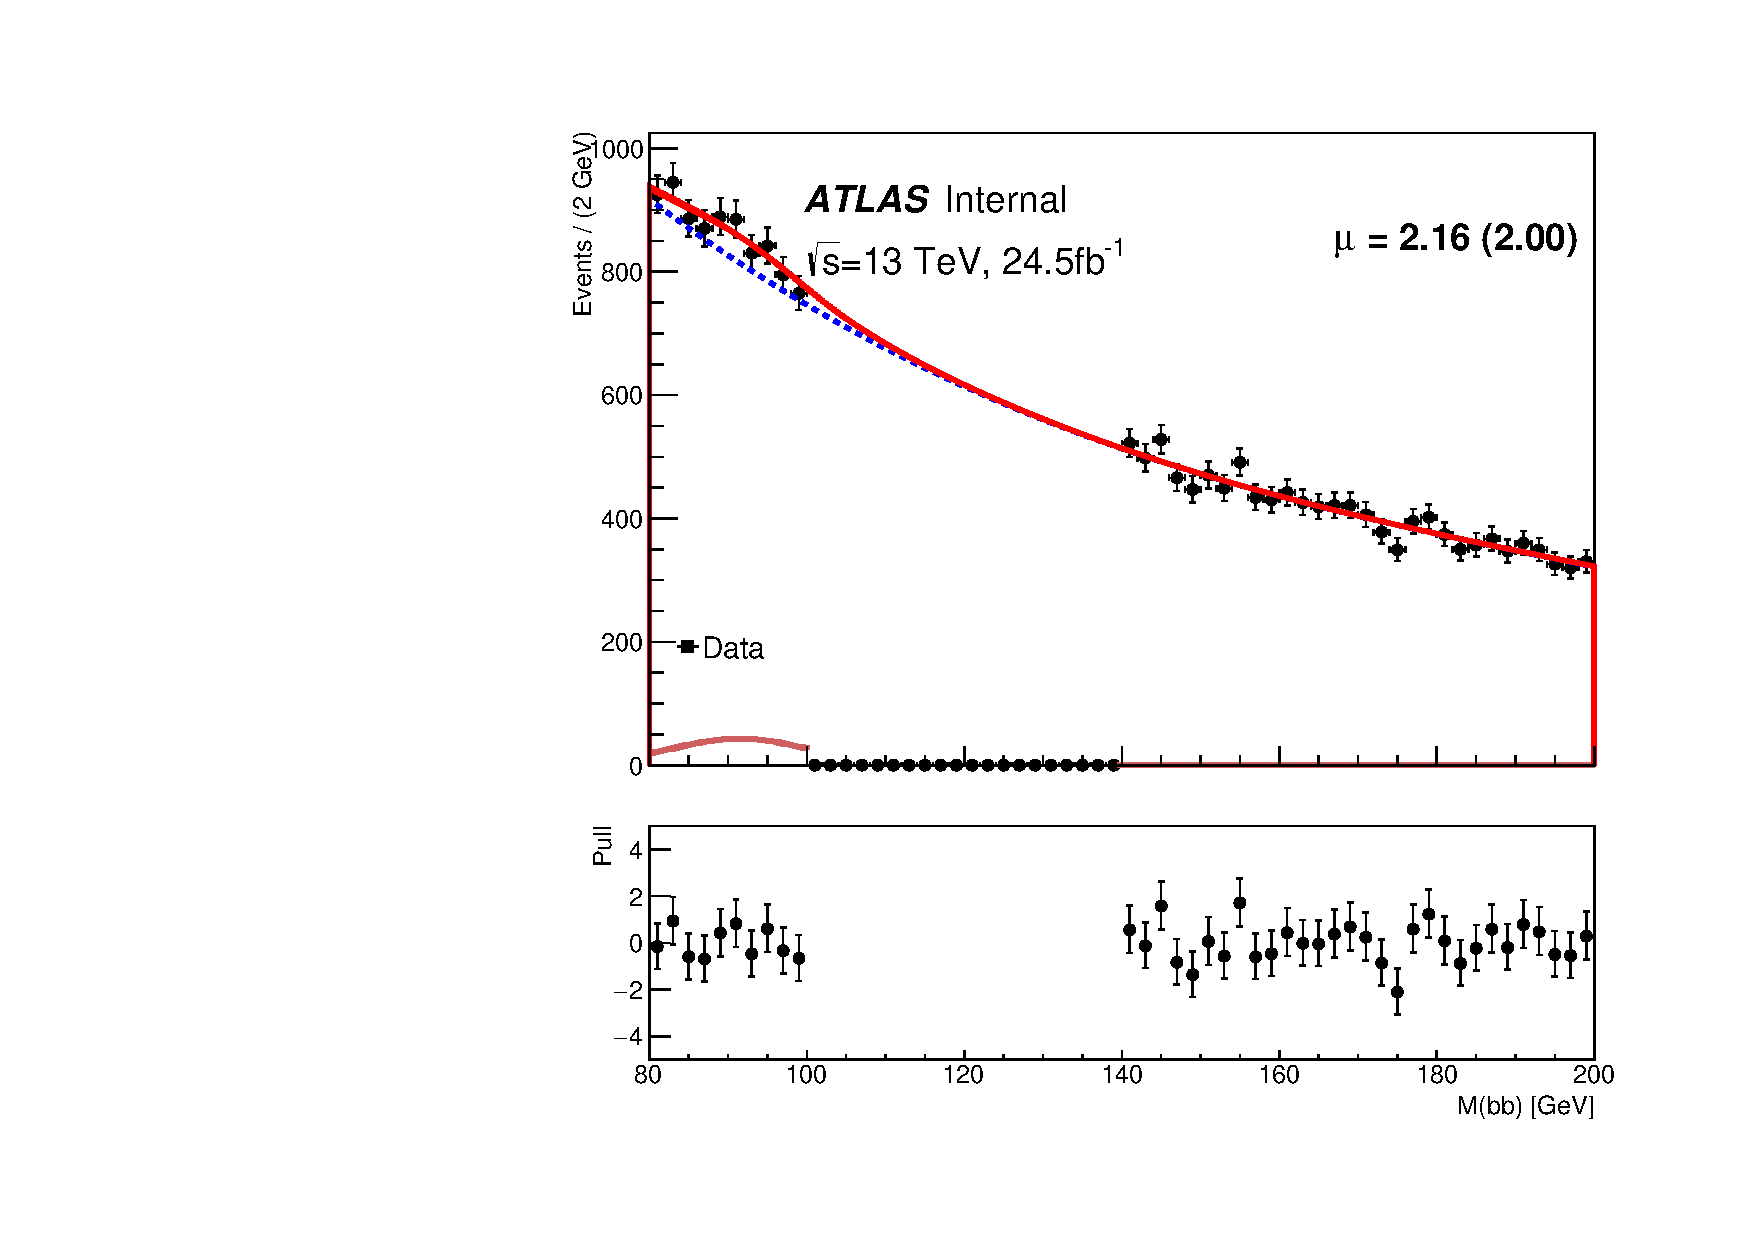
\includegraphics[width=0.24\textwidth]{figures/VBF/zunblind_testVBF_ICHEP_4cen_SRI.pdf}
% 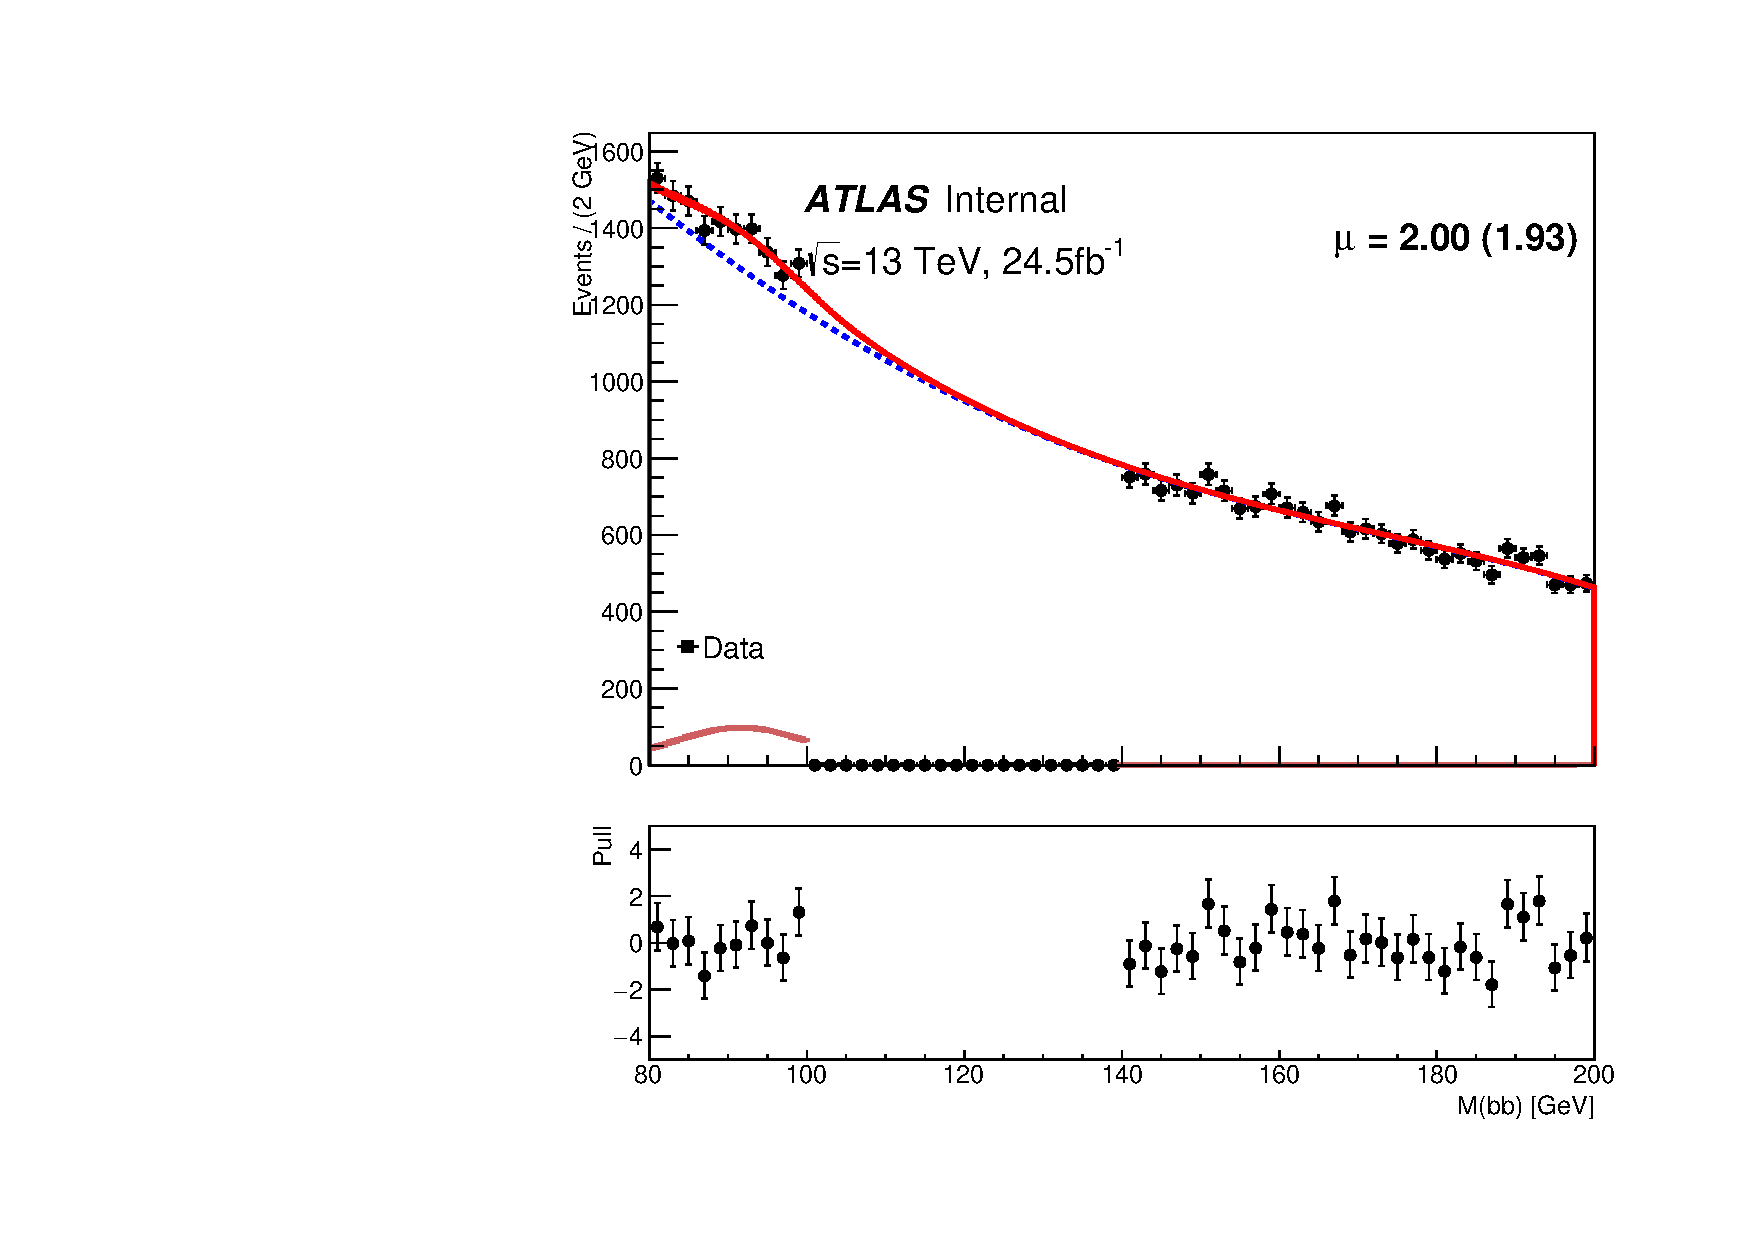
\includegraphics[width=0.24\textwidth]{figures/VBF/zunblind_testVBF_ICHEP_4cen_SRII.pdf}
% 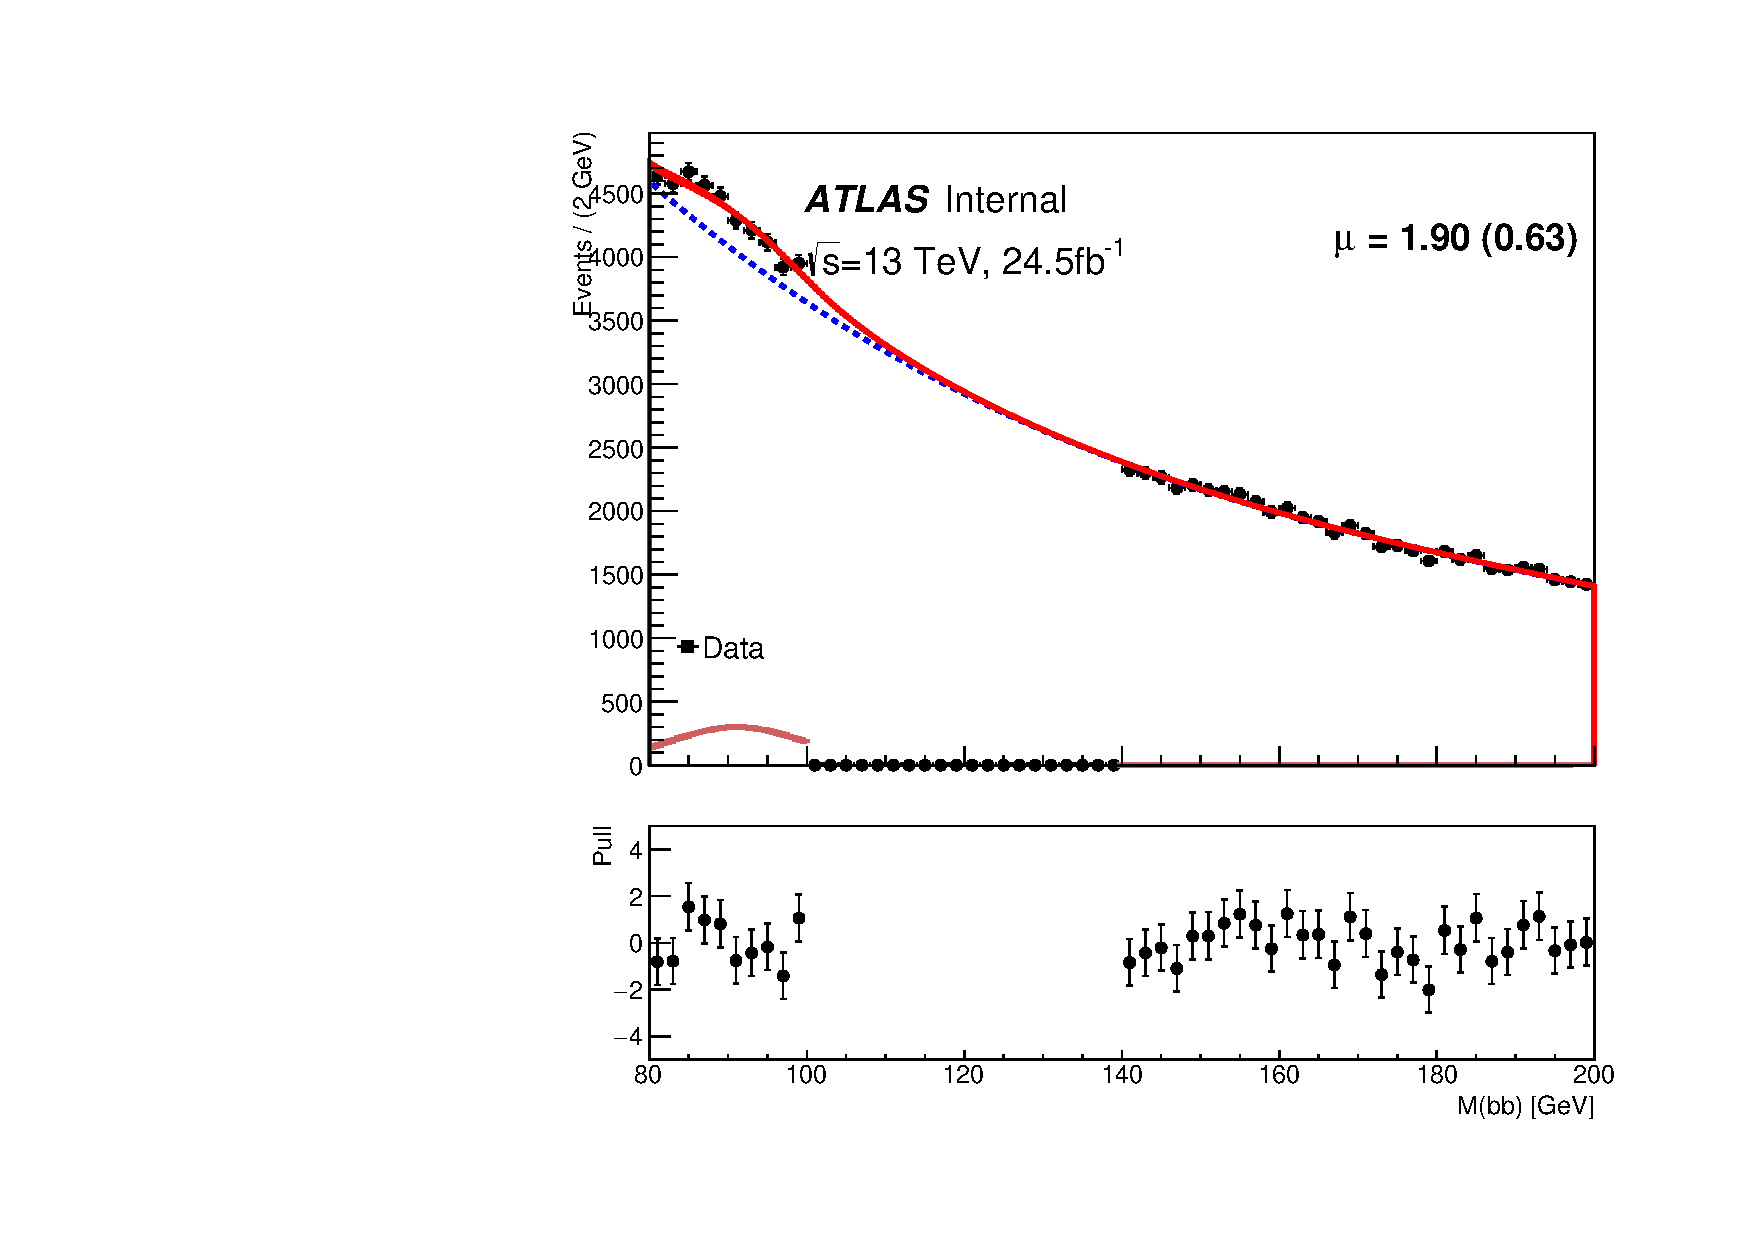
\includegraphics[width=0.24\textwidth]{figures/VBF/zunblind_testVBF_ICHEP_4cen_SRIII.pdf}
% 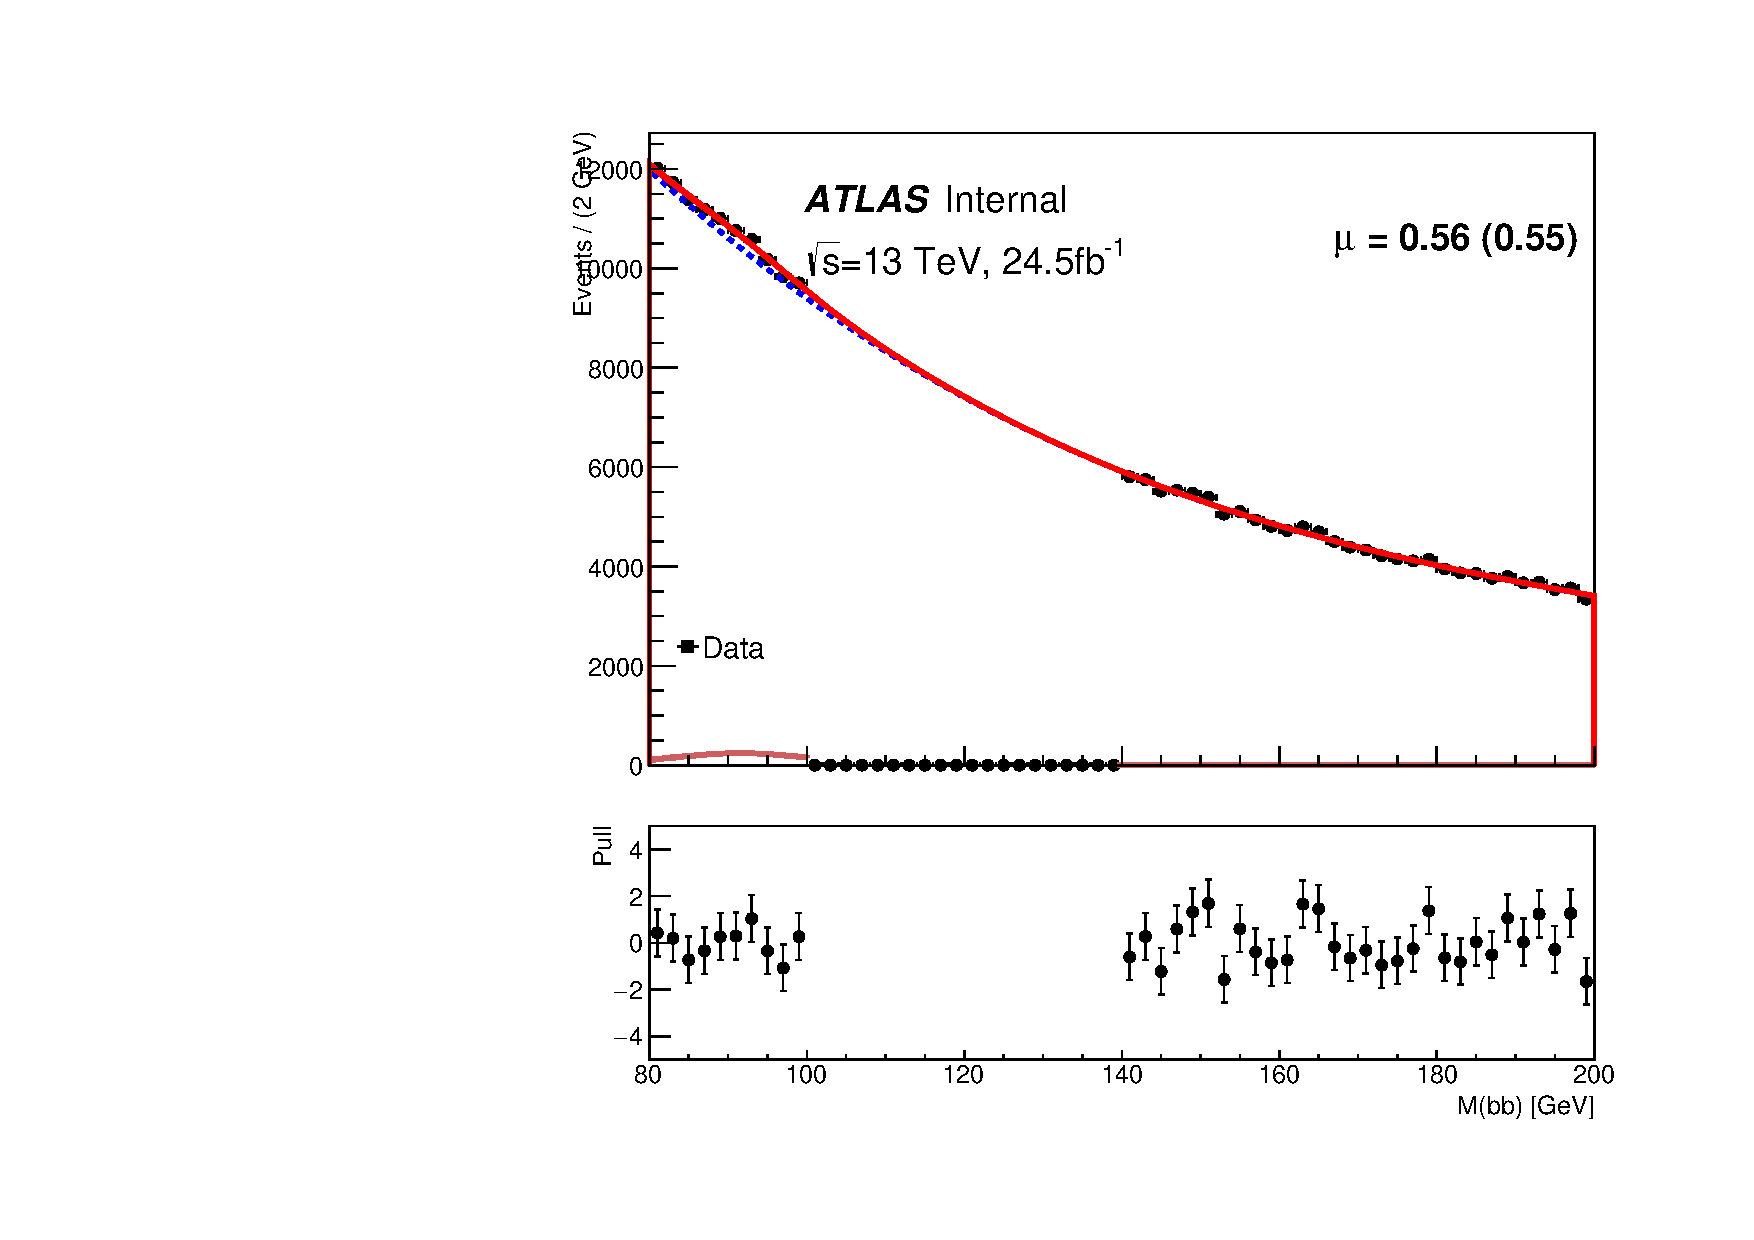
\includegraphics[width=0.24\textwidth]{figures/VBF/zunblind_testVBF_ICHEP_4cen_SRIV.pdf}\\
%\caption{Data and fit model comparison for sideband only \zjets{} fit in \twocentral (top) and \fourcentral channel (bottom) for SR I (left) to SR IV (right).  The data are the black points and the fit model (red), which comprises the continuum background (blue dashed line) and the Z contribution (light red histogram).}
%  \label{fig:vbf-zsidebandfit}
%\end{figure}


\subsection{Extraction of $\mu_{H}$}
\label{sec:vbf-higgsunblind}

The observed value of the Higgs signal strength is $2.7^{+2.2}_{-2.0}$, while the Asimov fit yields $\mu_{H}=1\pm 1.9$. The breakdown of the uncertainty is $\mu_H=2.7^{+1.9}_{-1.9}\textnormal{(stat)}^{+1.1}_{-0.6}\textnormal{(syst)}$ treating the NPs for the analytical background parameterization and normalization as well as the normalization of $Z$ contribution as statistical uncertainty.

%Figures~\ref{fig:vbf-higgsfit_2cen} and ~\ref{fig:vbf-higgsfit_4cen} show the resulting distributions for the \twocentral and \fourcentral channels. %displaying the residuals with respect to the continuum background fit on the bottom panel. % whereas Figures~\ref{fig:vbf-higgsfit_2cen_pull} and~\ref{fig:vbf-higgsfit_4cen_pull} show the pull values with respect to the full background model.  

%The pull values are shown in Figure~\ref{fig:vbf-higgsfitpull} for nuisance parameters with a post-fit impact of more than 4\%.  None of the nuisance parameters are strongly pulled. The largest uncertainty on $\mu_H$ comes from the theory uncertainty on the QCD scale, followed by the background parameterization and the jet energy resolution. The increase of the total uncertainty with respect to the expected value comes from the larger than expected background normalization as well as an increase of the signal systematics which scales as the size of the $\mu_H$. 

The fitted $Z$ values are shown in Table~\ref{tab:zfullfit} for each SR.  Reductions of 30--60\% of the $\mu_Z$ uncertainties are observed with respect to the sideband only fit. A statistical combination of all the channels, as described in Equation~\ref{eqn:zsig}, yields an effective $\mu_Z = 1.2 \pm 0.2$ with a combined $\chi^2/$ndof of 1.05 with a probability of 38.8\%.  

\begin{table}[htbp]
\centering
\caption{Floating Z normalization parameters in full mass range fit.}
\label{tab:zfullfit}
\begin{tabular}{|l|c|c|}
\hline
Channel      & $\mu_{Z}$   & $\chi^2/ndof$ \\ \hline
2 cen SR I   & 2.2$\pm$0.7  & 0.9      \\ \hline
2 cen SR II  & 0.4$\pm$0.4  & 0.7        \\ \hline
4 cen SR I   & 0.3$\pm$1.1  & 0.7         \\ \hline
4 cen SR II  & 1.2$\pm$0.6  & 0.7        \\ \hline
4 cen SR III & 1.4$\pm$0.4  & 0.7         \\ \hline
4 cen SR IV  & 0.9$\pm$0.2  & 0.8          \\ \hline
\end{tabular}
\end{table}


%\begin{figure}[htbp]
%  \centering
% 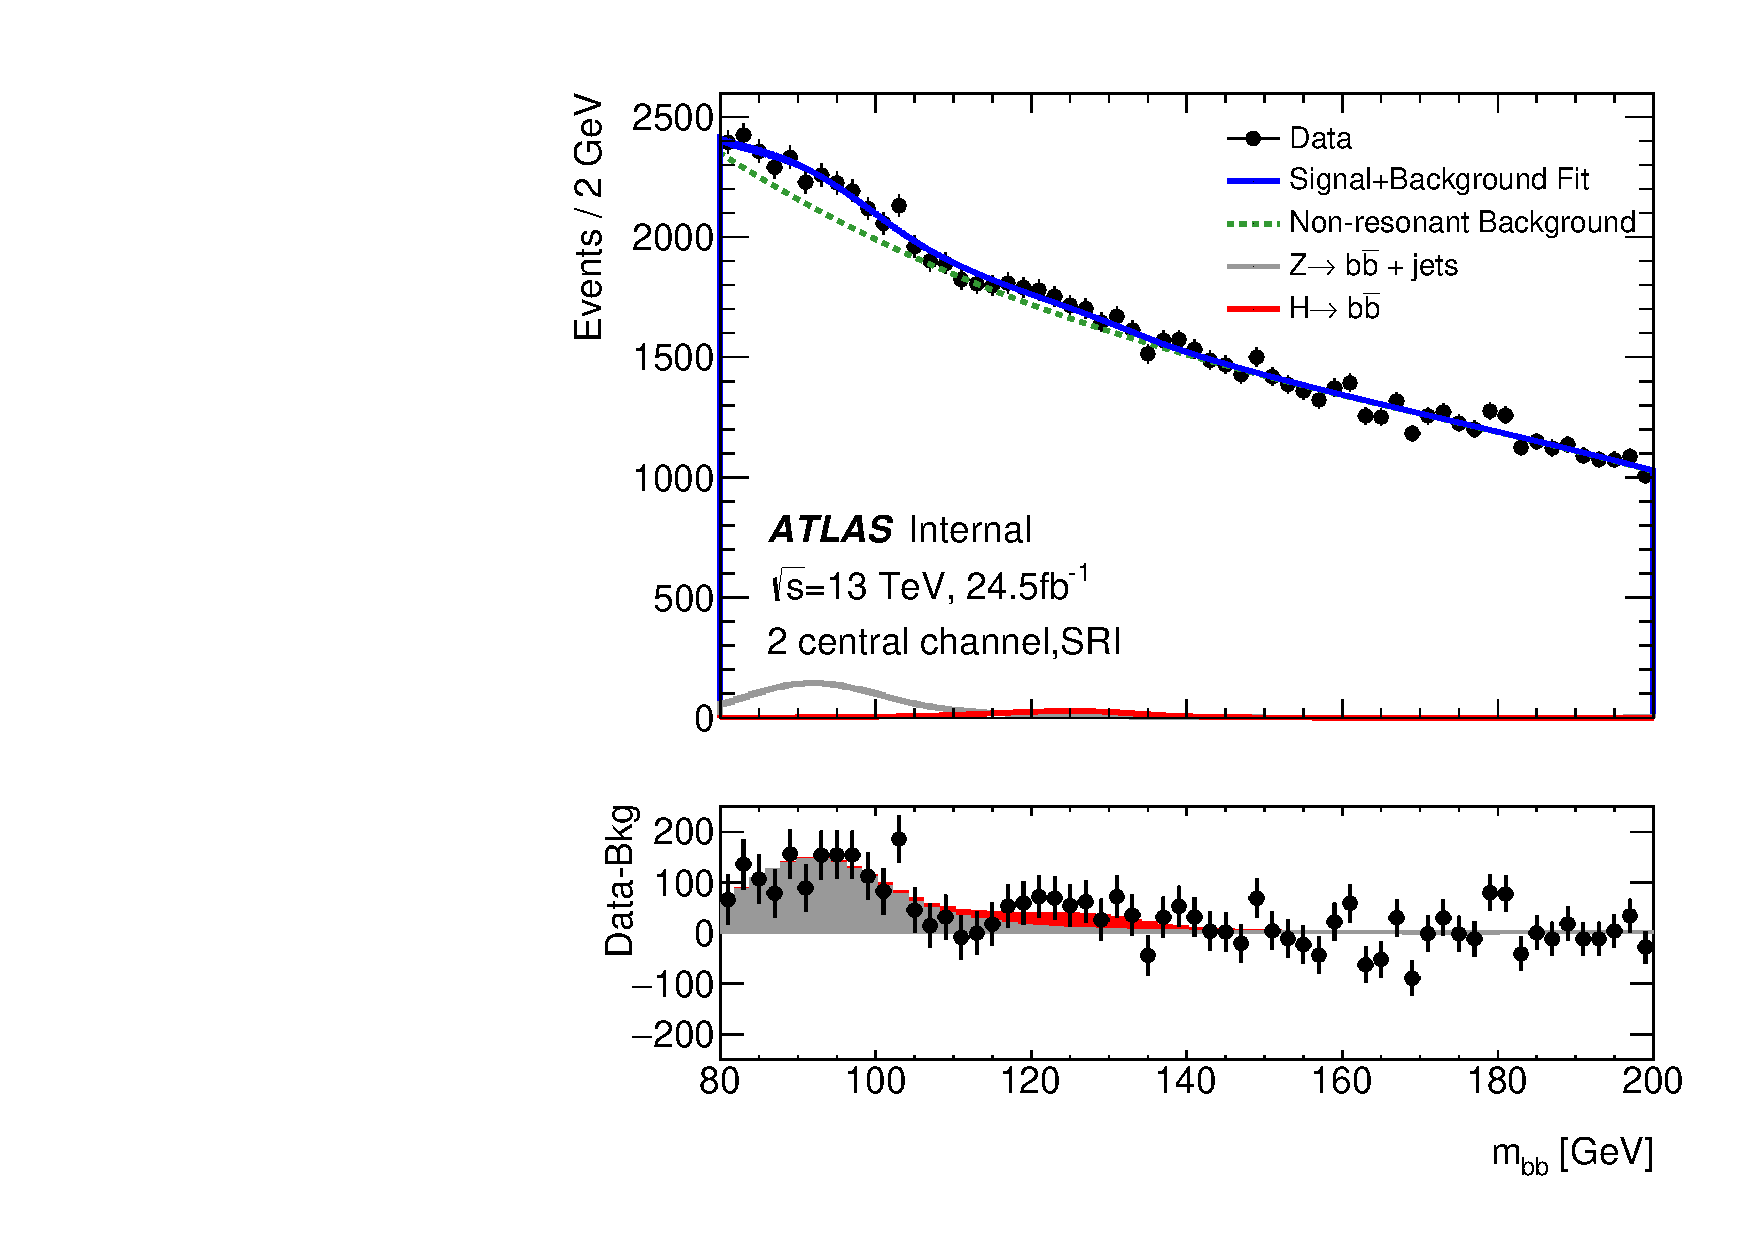
\includegraphics[width=0.48\textwidth]{figures/VBF/unblind_testVBF_ICHEP_2cen_SRI.pdf}
% 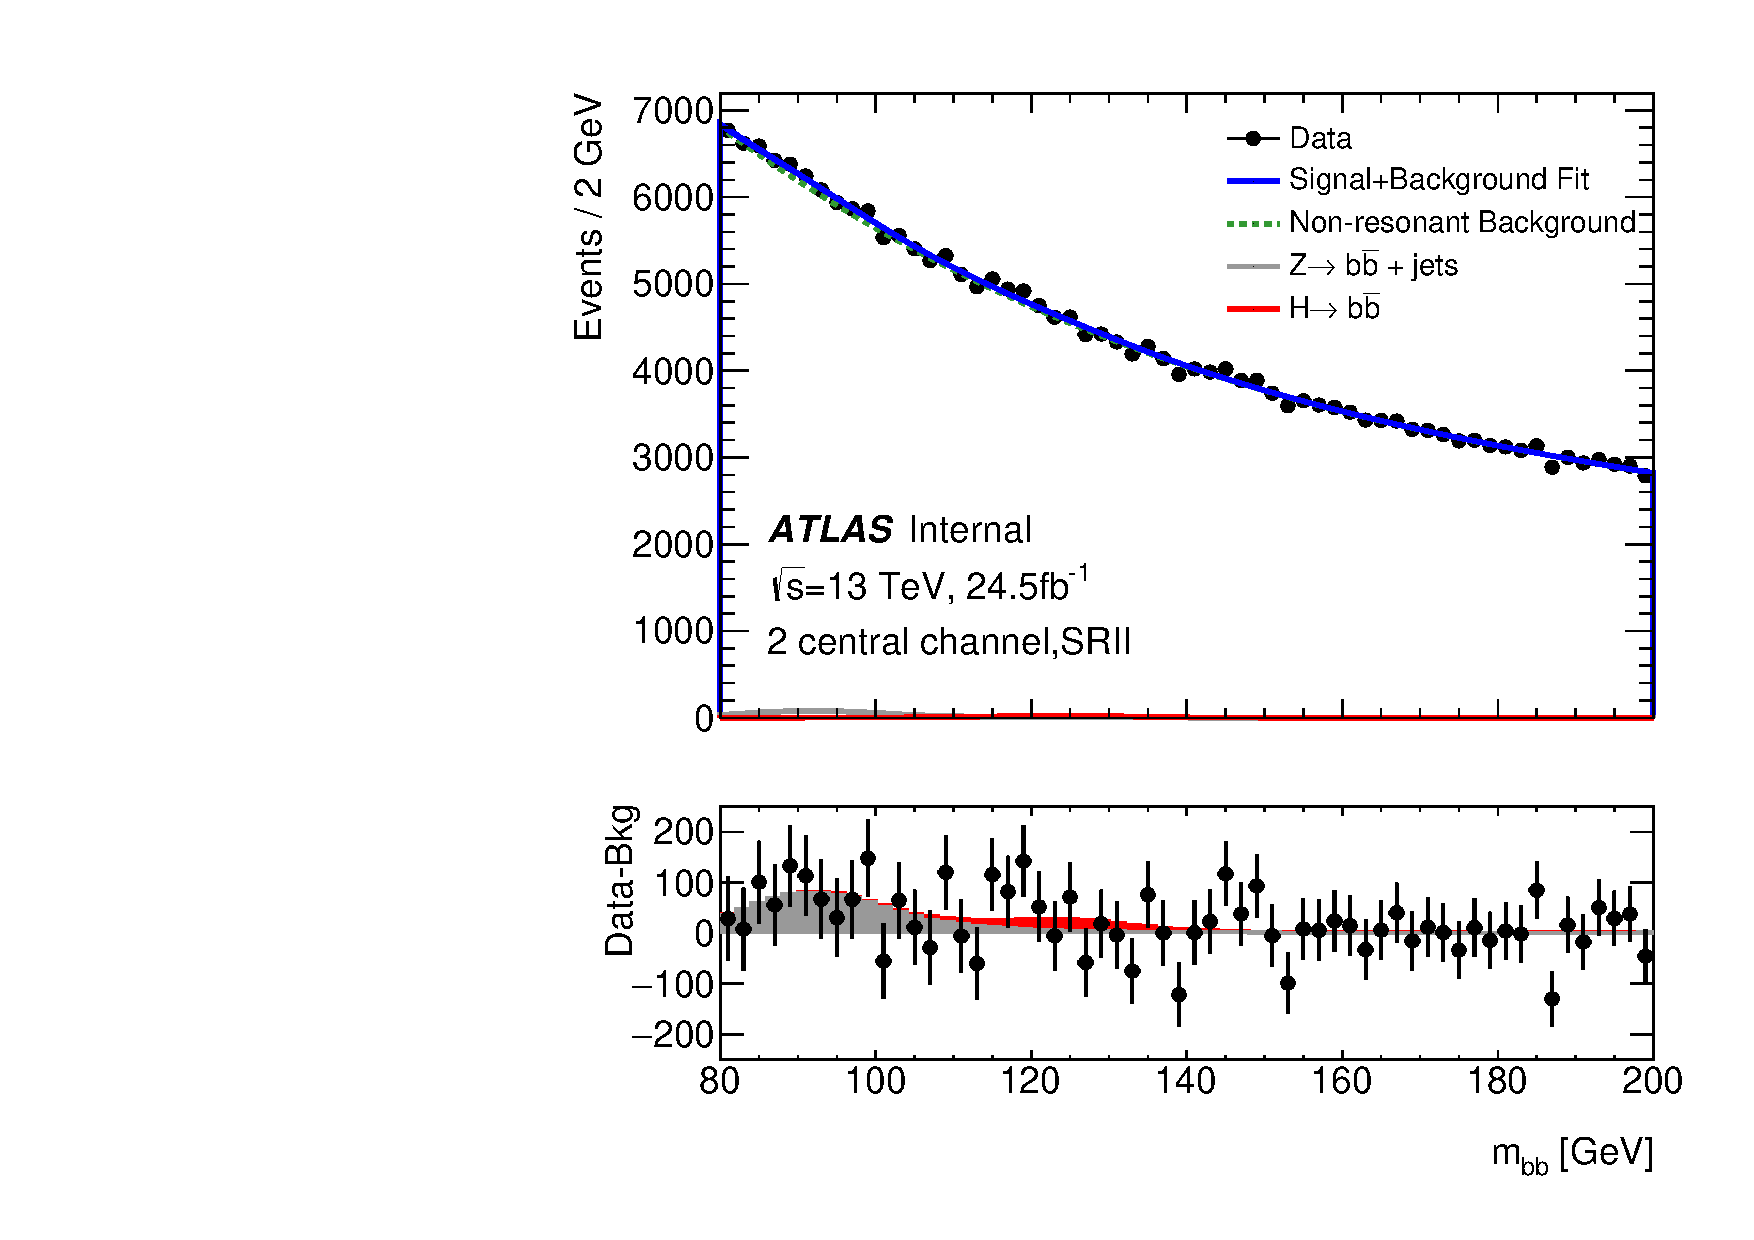
\includegraphics[width=0.48\textwidth]{figures/VBF/unblind_testVBF_ICHEP_2cen_SRII.pdf}\\
%\caption{Data and fit model comparison for profile likelihood fit in the \twocentral channel signal regions.  The fitted continuum background is shown with at  dashed green line, the fitted $Z$ signal in green, and the fitted Higgs signal in red.  The total fit is displayed as the blue line.  The bottom panels show the residual of the data with respect to the continuum background fit, and the fitted $Z$ signal (grey) and Higgs signal (red) are also displayed. }
%  \label{fig:vbf-higgsfit_2cen}
%\end{figure}
%
%\begin{figure}[htbp]
%  \centering
% 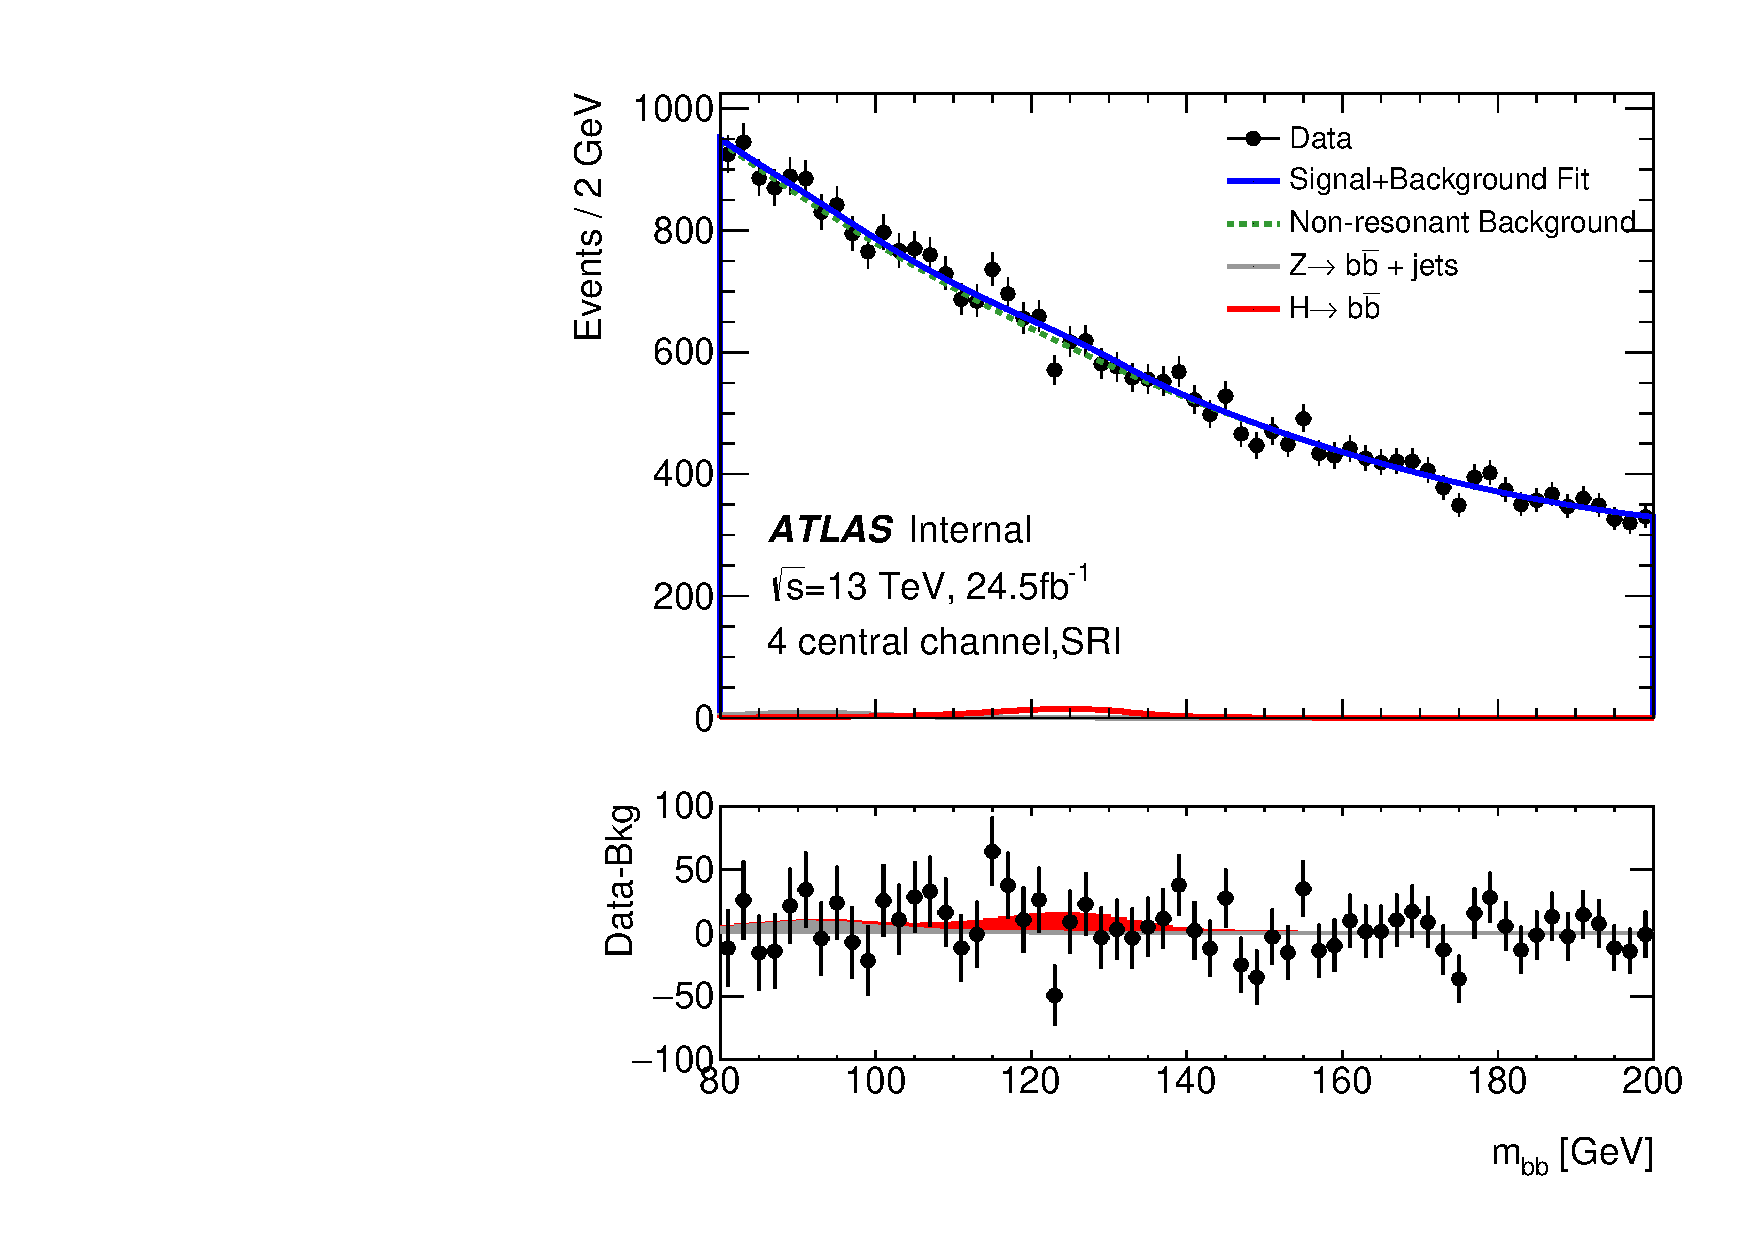
\includegraphics[width=0.48\textwidth]{figures/VBF/unblind_testVBF_ICHEP_4cen_SRI.pdf}
% 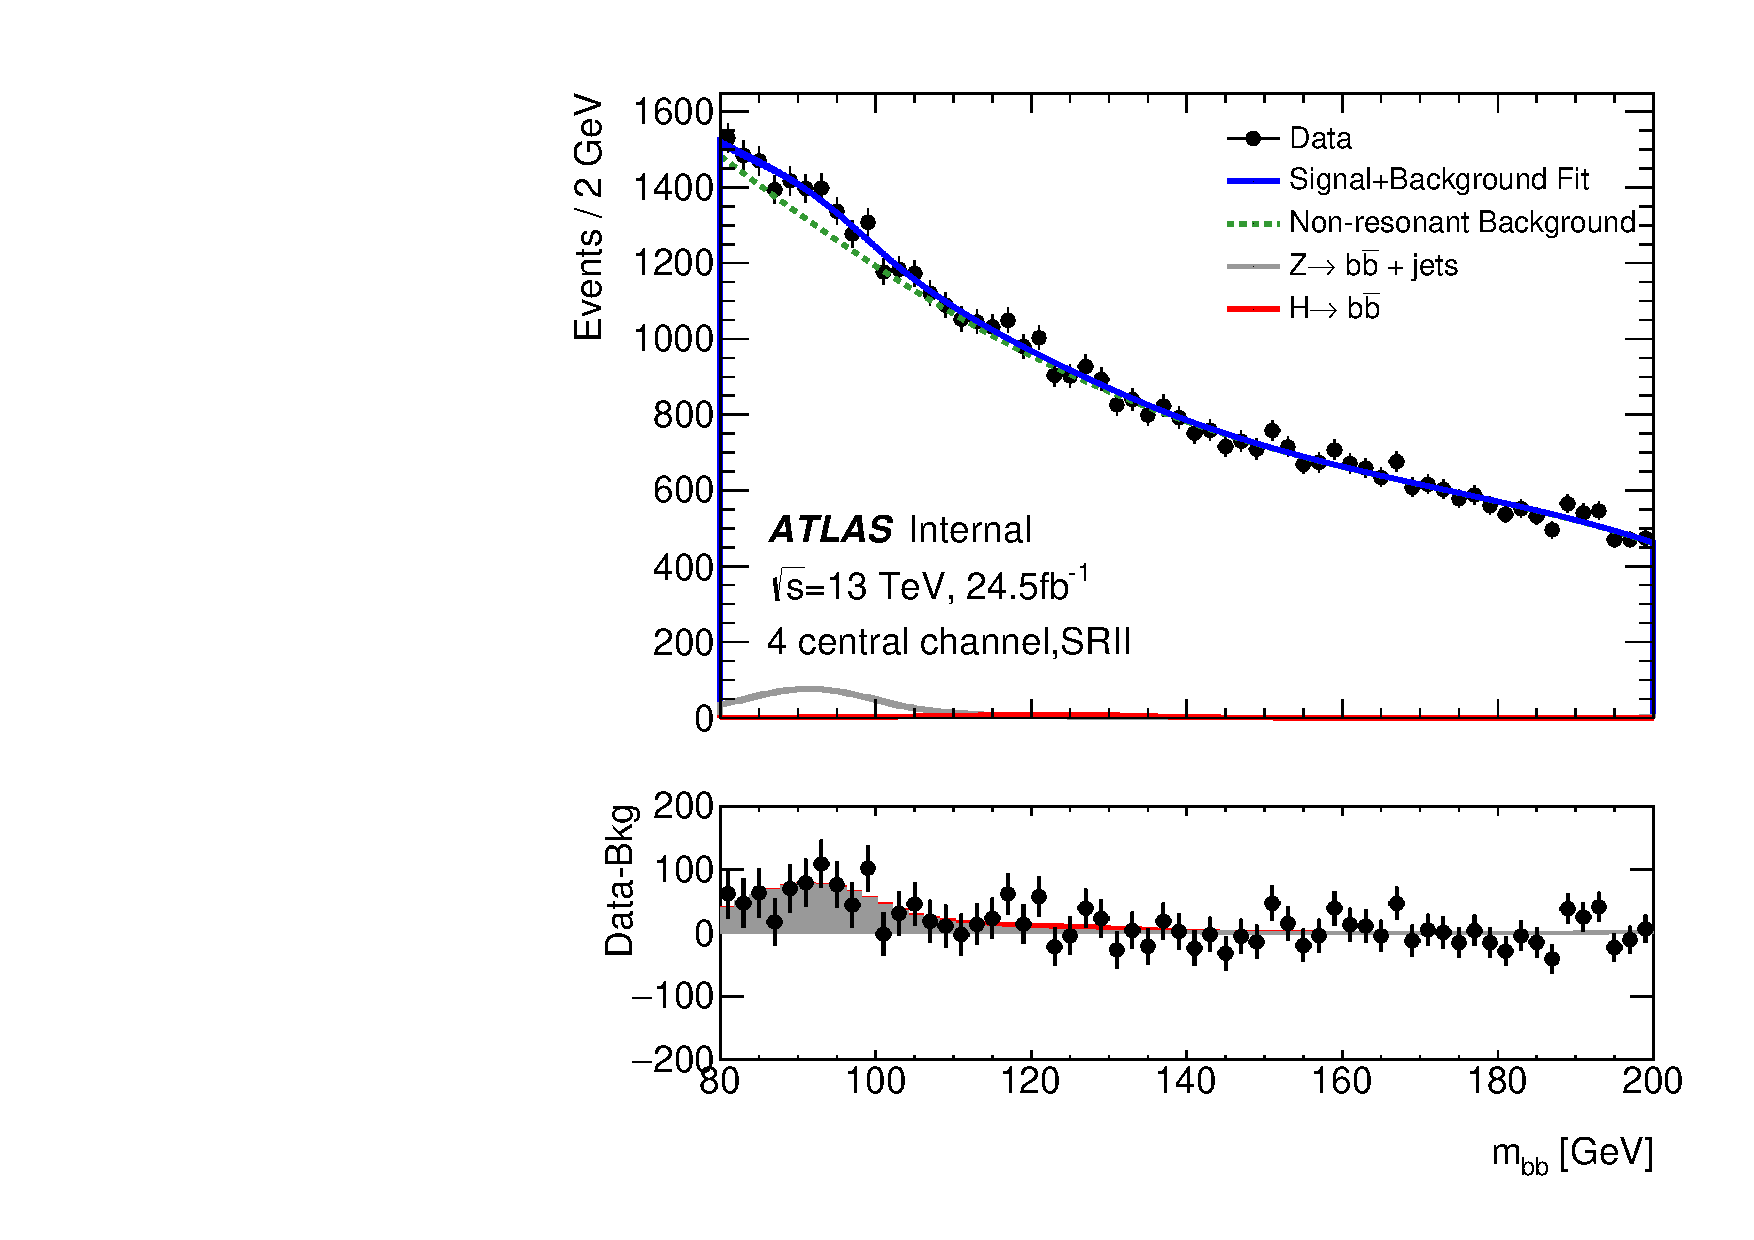
\includegraphics[width=0.48\textwidth]{figures/VBF/unblind_testVBF_ICHEP_4cen_SRII.pdf}\\
% 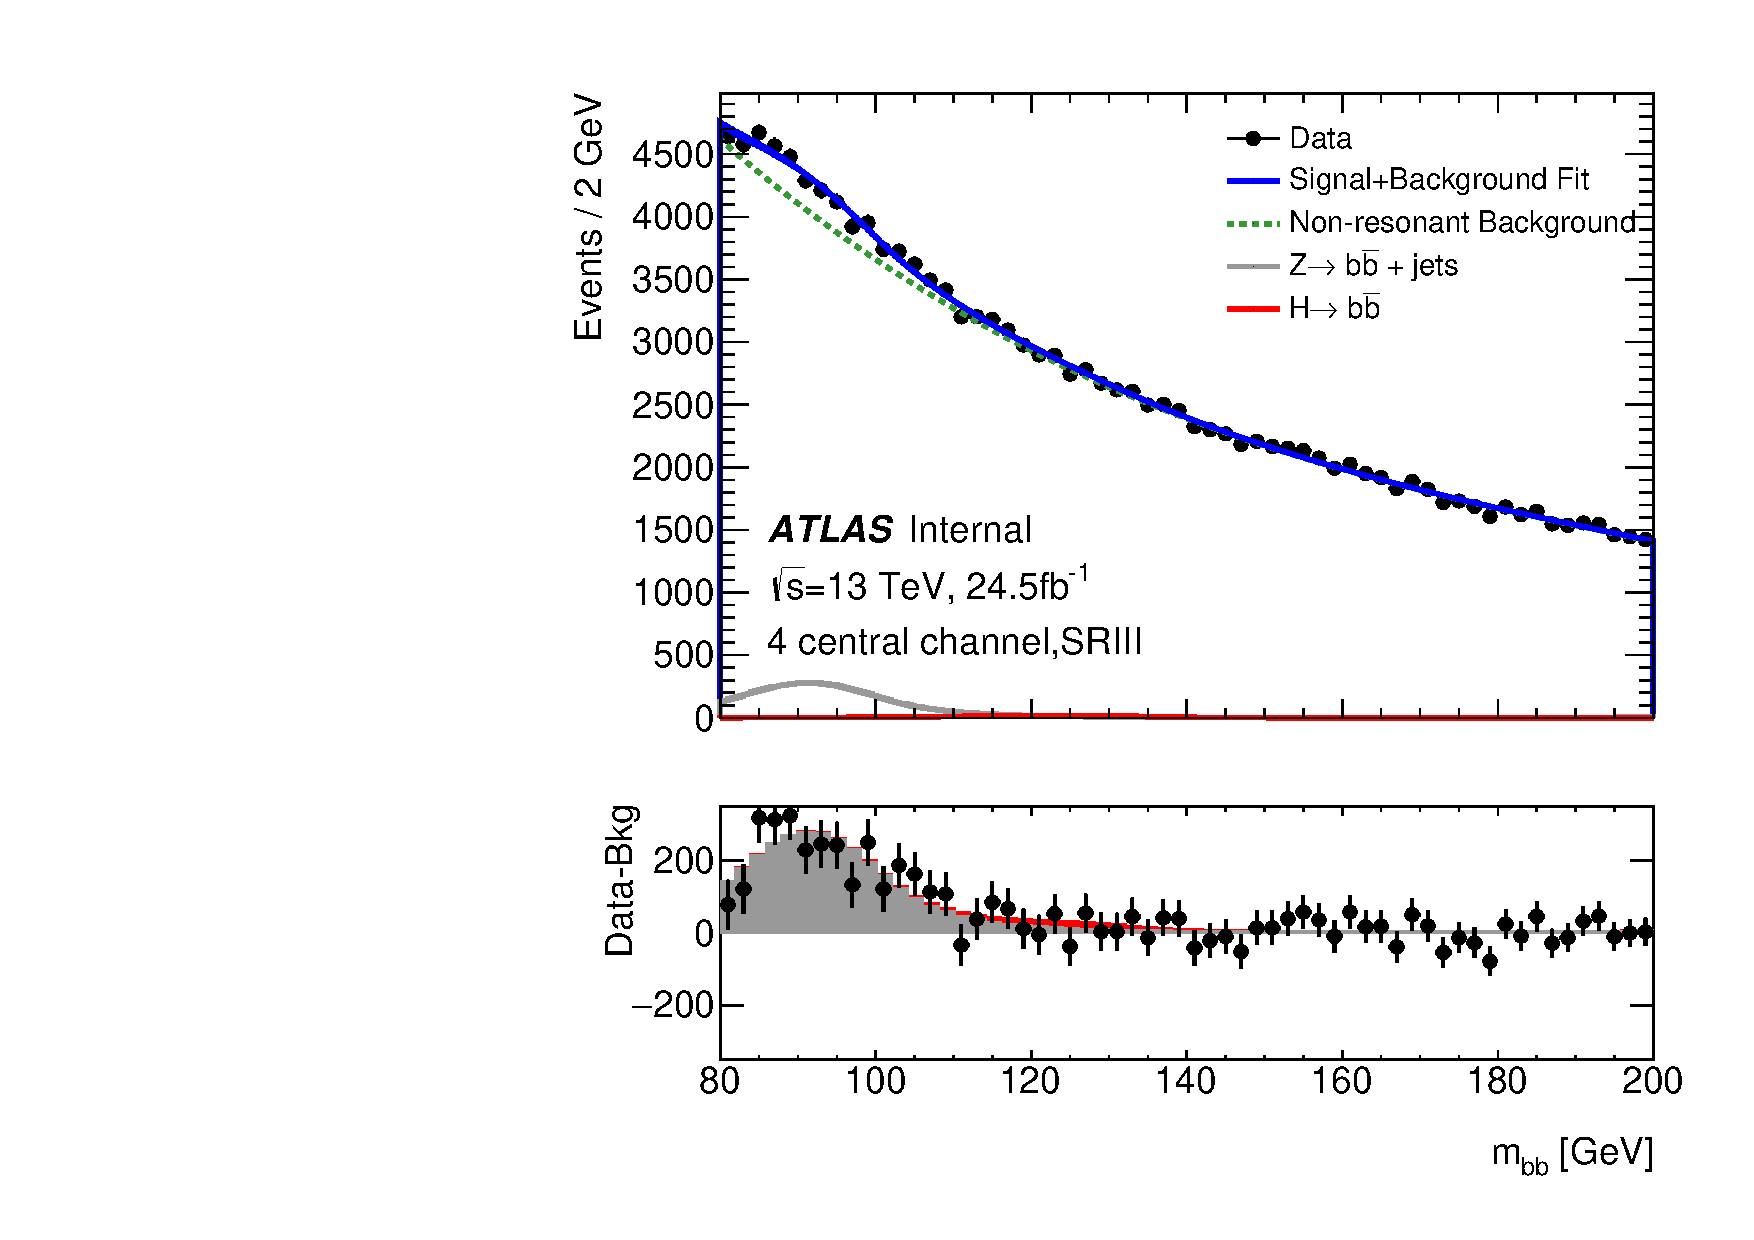
\includegraphics[width=0.48\textwidth]{figures/VBF/unblind_testVBF_ICHEP_4cen_SRIII.pdf}
% 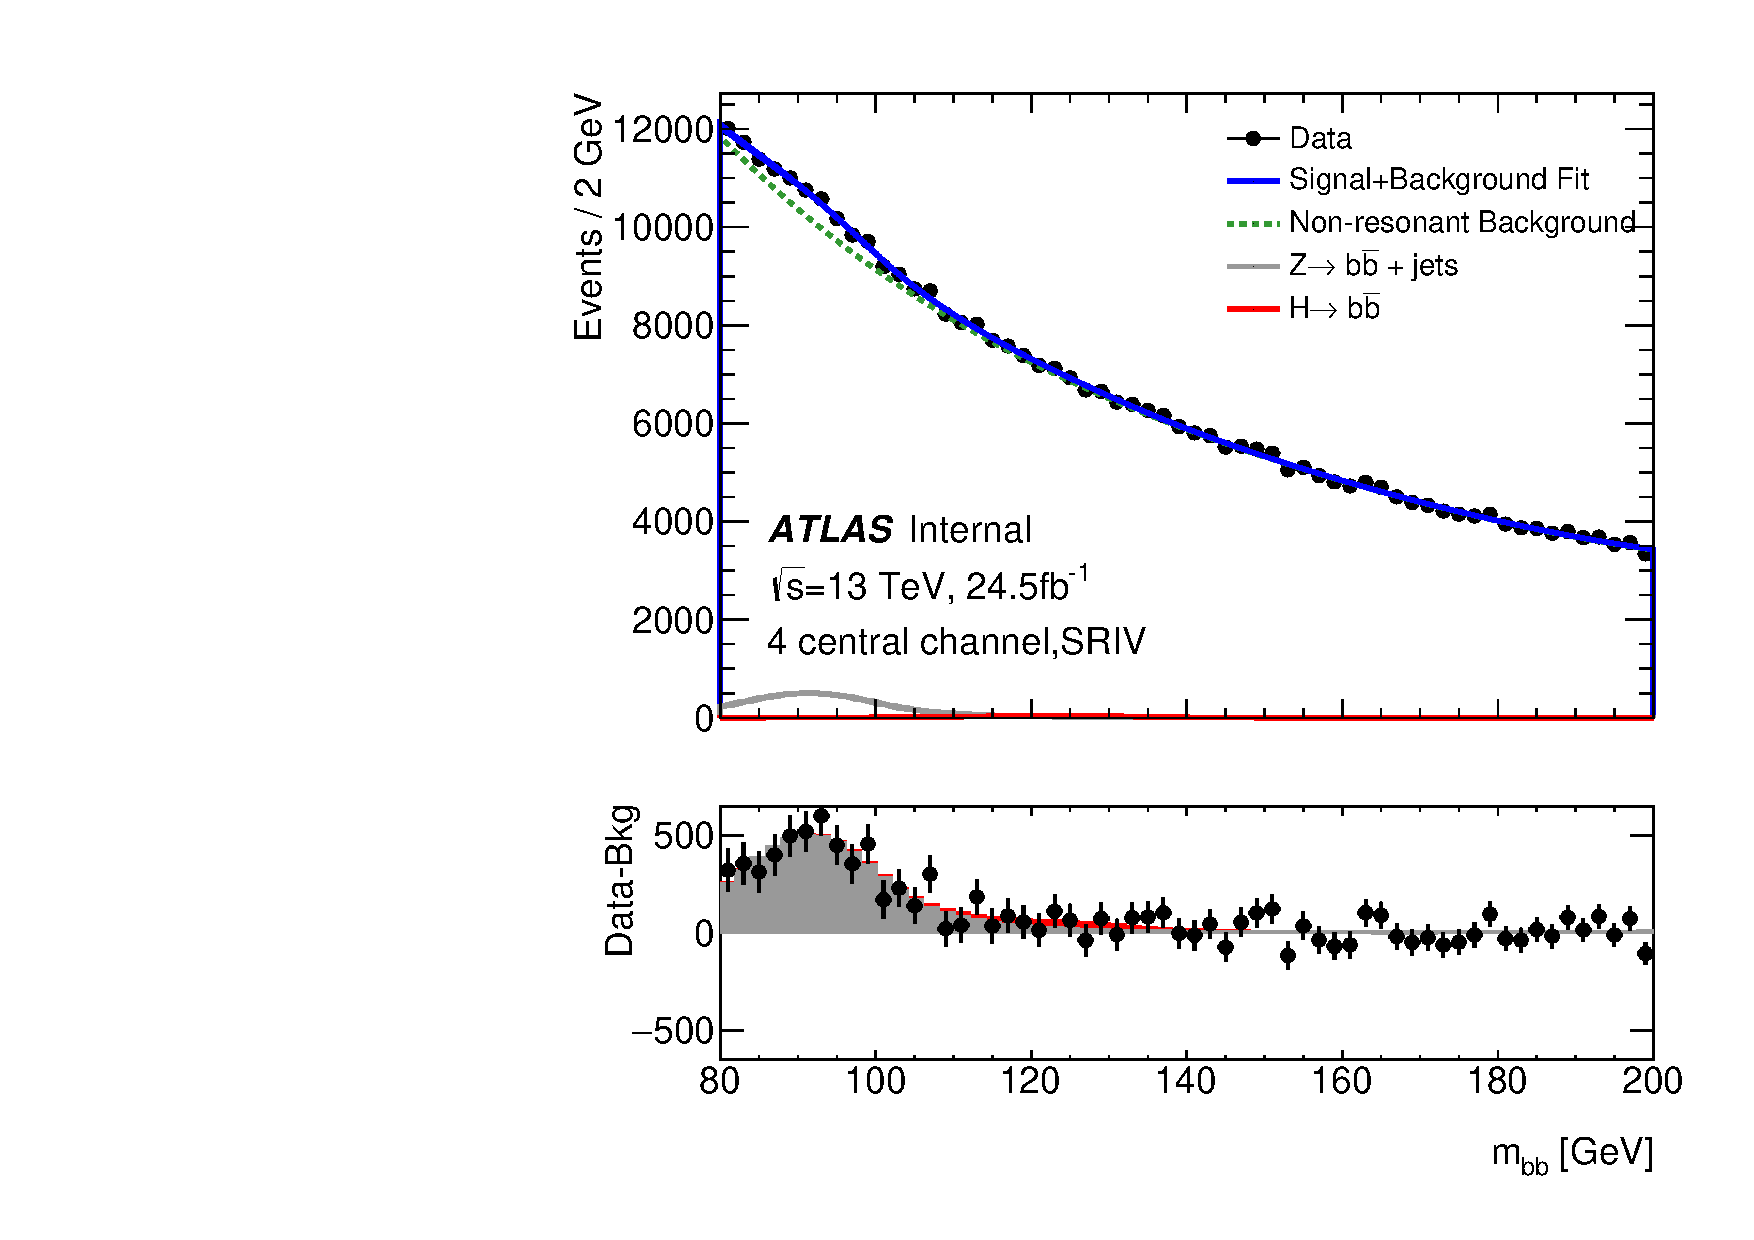
\includegraphics[width=0.48\textwidth]{figures/VBF/unblind_testVBF_ICHEP_4cen_SRIV.pdf}\\
%\caption{Data and fit model comparison for profile likelihood fit in the \fourcentral channel signal regions. The fitted continuum background is shown with at  dashed green line, the fitted $Z$ signal in green, and the fitted Higgs signal in red.  The total fit is displayed as the blue line.  The bottom panels show the residual of the data with respect to the continuum background fit, and the fitted $Z$ signal (grey) and Higgs signal (red) are also displayed.}
%  \label{fig:vbf-higgsfit_4cen}
%\end{figure}


\subsection{Extraction of $\mu_{VBF}$}
\label{sec:vbf-higgsunblindvbf}
A different interpretation of the analysis is the extraction of $\mu_{VBF}$ signal strength.
The fit procedure follows the same way as the extraction of $\mu_{H}$, except we only float
the $VBF$ signal in the fit while fixing the yield of all other Higgs modes, i.e. ggF,
ttH and VH to their Standard Model predictions (with uncertainties applied).
The Asimov fit yields $\mu_{VBF}=1\pm 2.8$. The unblinded value of the VBF Higgs signal
strength is $4.1^{+3.2}_{-2.9}$. The breakdown of the uncertainty
is $\mu_{VBF}=4.1^{+2.8}_{-2.8}\textnormal{(stat)}^{+1.5}_{-0.8}\textnormal{(syst)}$ treating
the NPs for the analytical background parameterization and normalization as well as
the normalization of $Z$ contribution as statistical uncertainty.


\subsubsection{Combination with VBF$+\gamma$ Analysis}
\label{sec:vbf-higgscomb}

The combination of the all-hadronic VBF analysis and the
VBF$+\gamma$ analysis~\cite{vbfplusgammaint} is performed
by a simultaneous likelihood fit to both datasets. The Higgs signal strength is
treated as correlated across all analysis regions,
the $Z$ contributions are extracted as described in the respective analyses.
As described in Section~\ref{sec:vbf-presel}, overlap between the two samples is removed.

The combined fit yields $\mu_H = 2.5^{+1.4}_{-1.3}$ corresponding to an observed significance
of $1.9\sigma$ ($0.8\sigma$ expected). The $VBF$ signal only extraction is also performed combining two analyses similar to \ref{sec:vbf-higgsunblindvbf}. The combined fit yields $\mu_{VBF} =3.0^{+1.7}_{-1.6}$ corresponding to an observed significance of $1.9\sigma$ ($0.7\sigma$ expected). The data and fit model comparisons for $\mu_{VBF}$ extraction are shown in Fig.\ref{fig:higgsfit_2cen},\ref{fig:higgsfit_4cen},\ref{fig:mbb_postfit_photon}.

The extractions of $\mu_{H}$ and $\mu_{VBF}$ for separate fits of both all-hadronic and photon analysis and the combination fit are summarized in Fig.\ref{fig:vbf-summary}.


\begin{figure}[htbp]
  \centering
 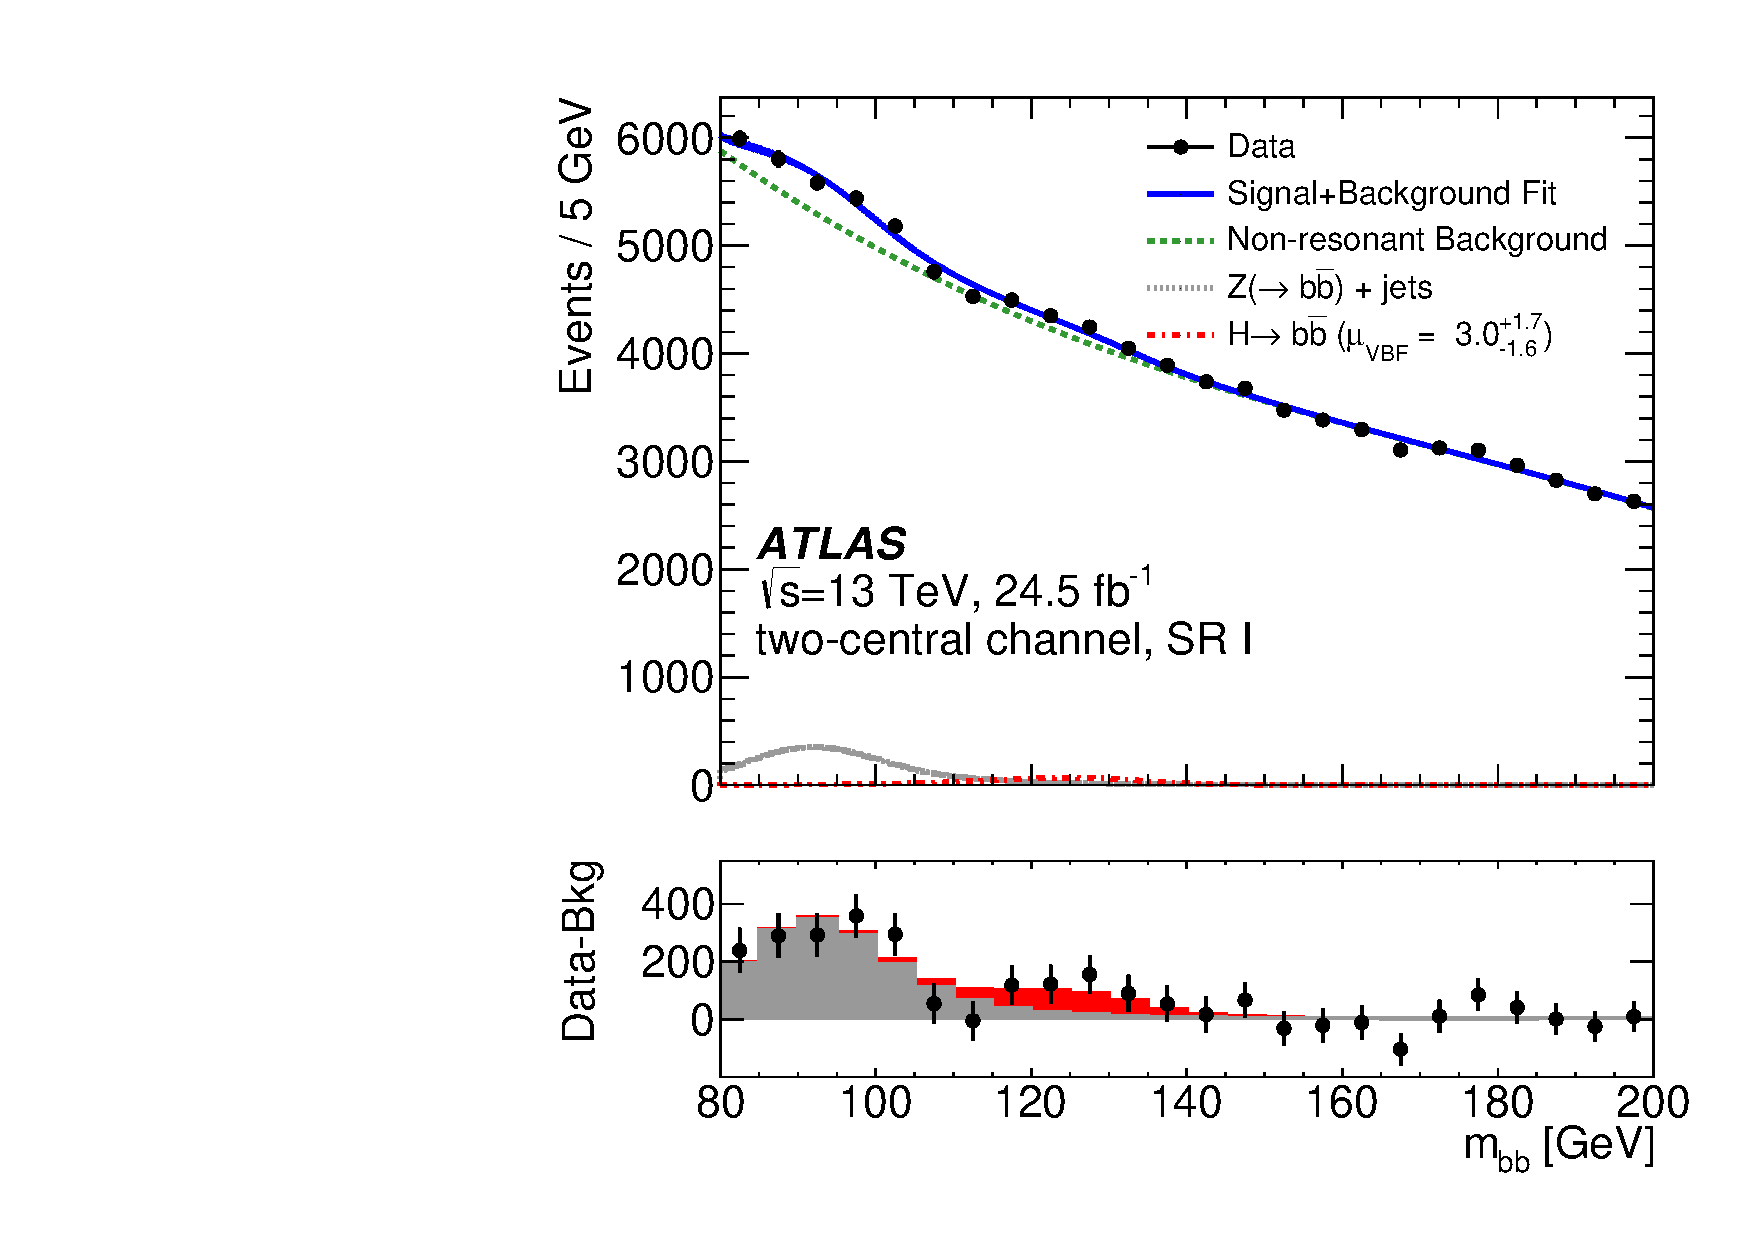
\includegraphics[width=0.48\textwidth]{figures/VBF/comb_vbfonly_testVBF_ICHEP_2cen_SRI_vbfincl.pdf}
 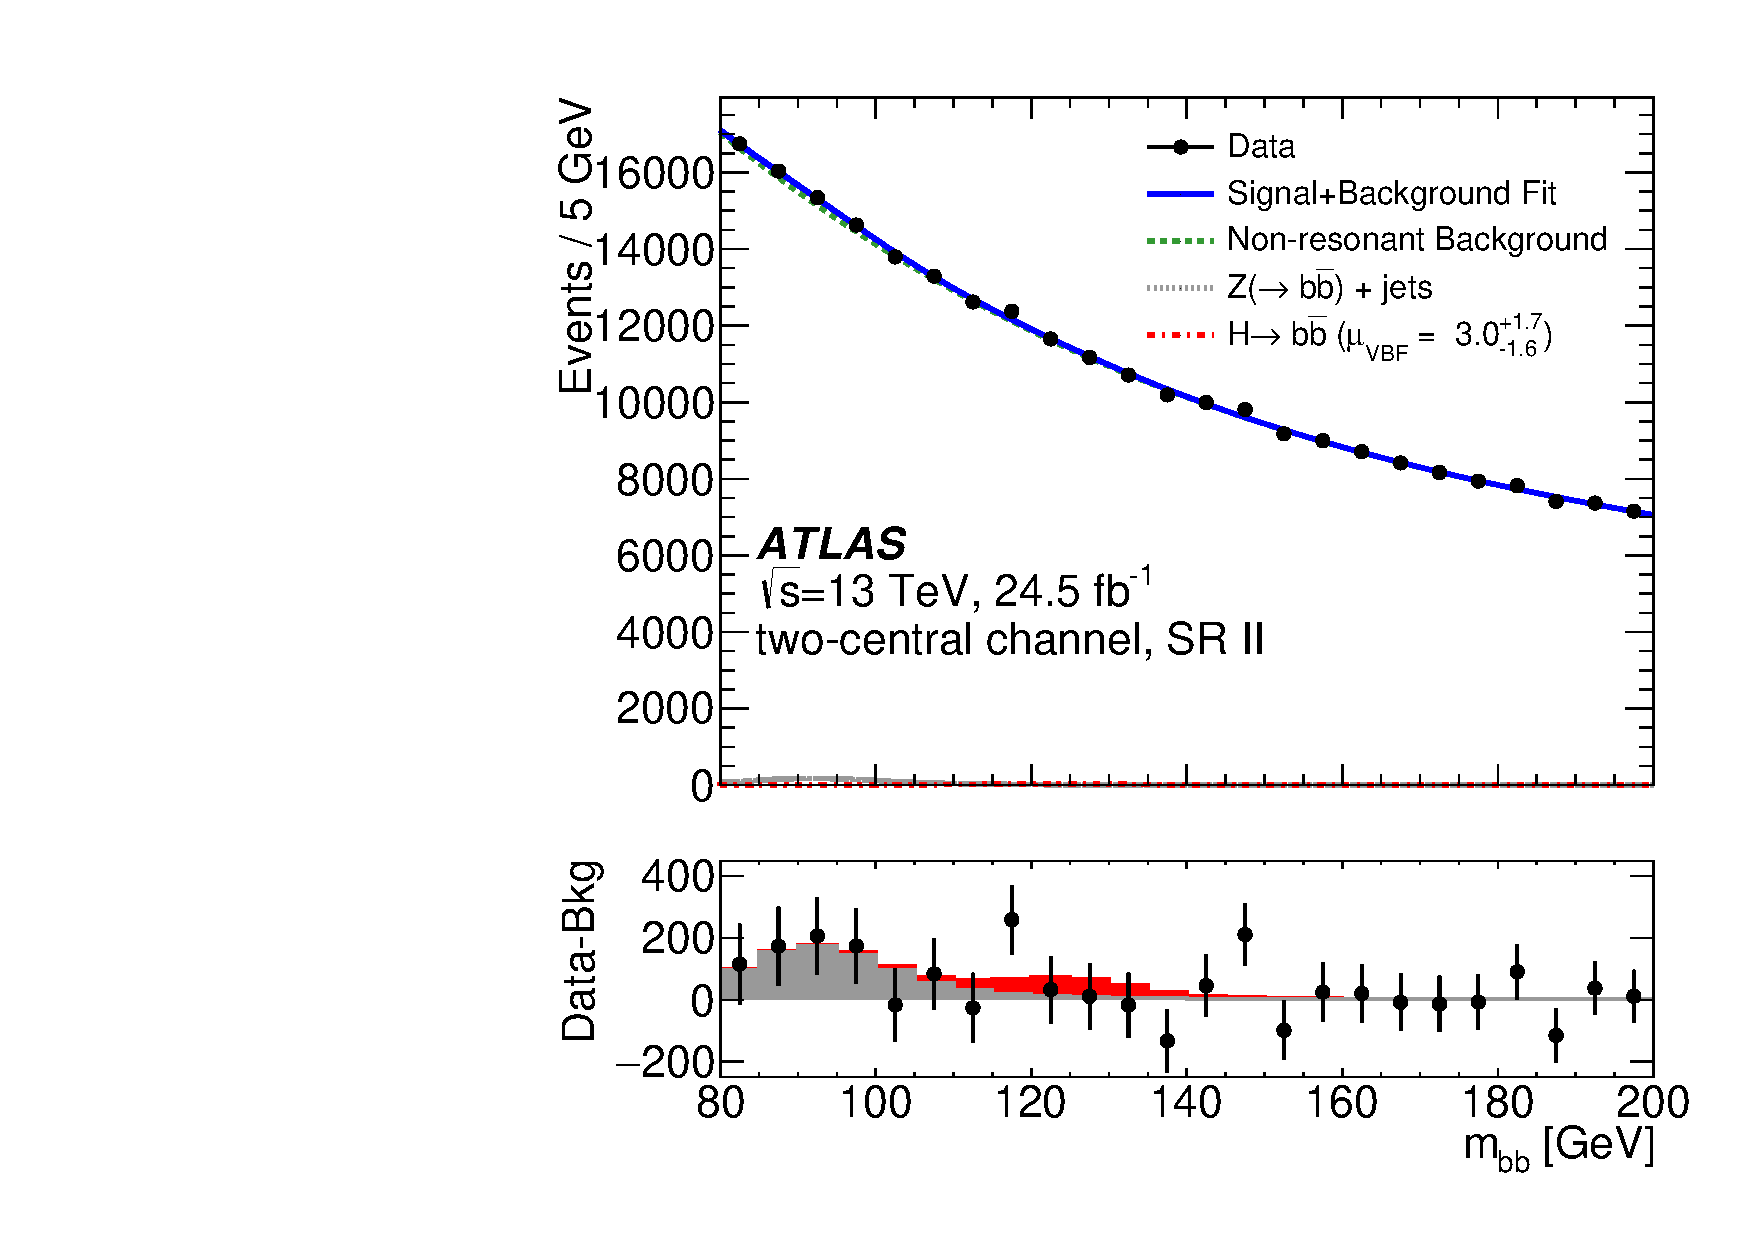
\includegraphics[width=0.48\textwidth]{figures/VBF/comb_vbfonly_testVBF_ICHEP_2cen_SRII_vbfincl.pdf}\\

\caption{Data and fit model comparison for the combined fit of $\mu_{VBF}$ extraction in the \twocentral channel}
  \label{fig:higgsfit_2cen}
\end{figure}

\begin{figure}[htbp]
  \centering
  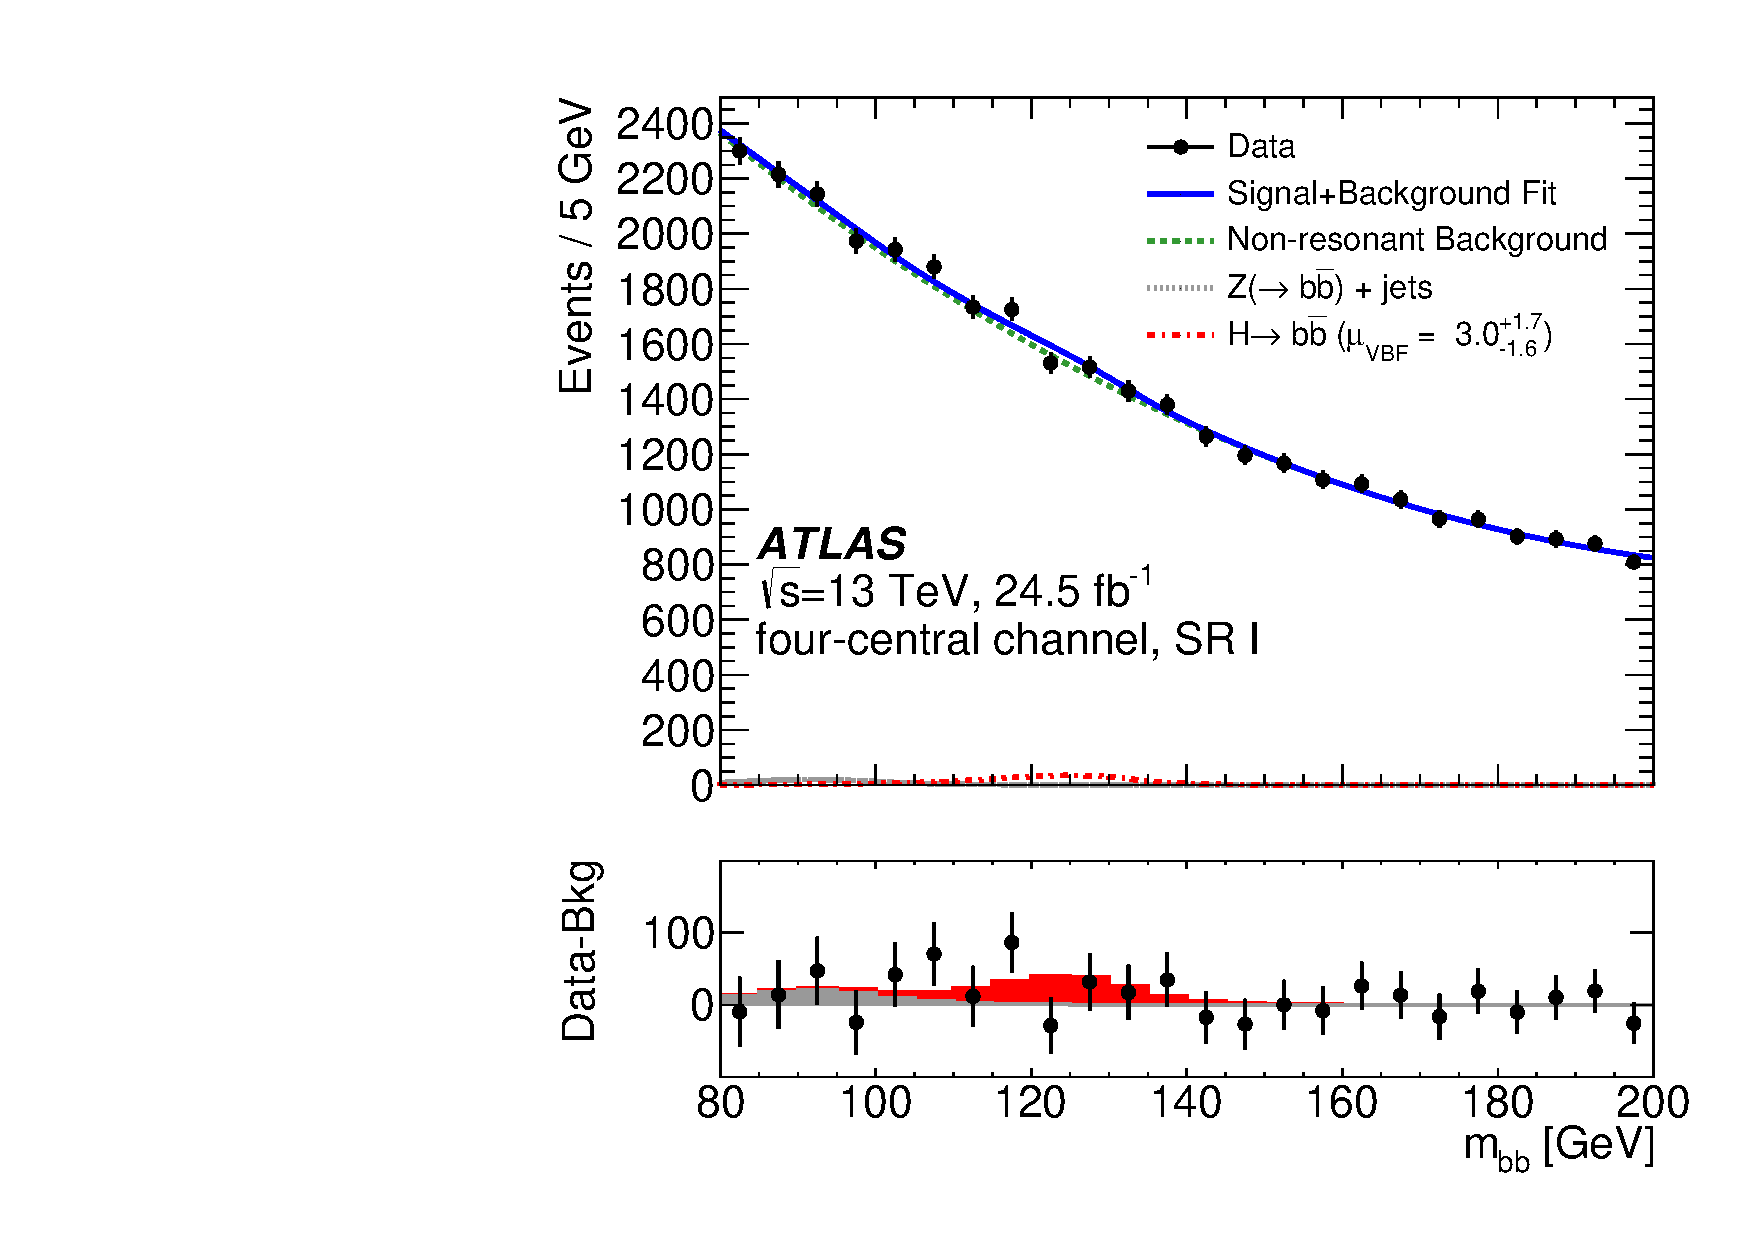
\includegraphics[width=0.48\textwidth]{figures/VBF/comb_vbfonly_testVBF_ICHEP_4cen_SRI_vbfincl.pdf}
 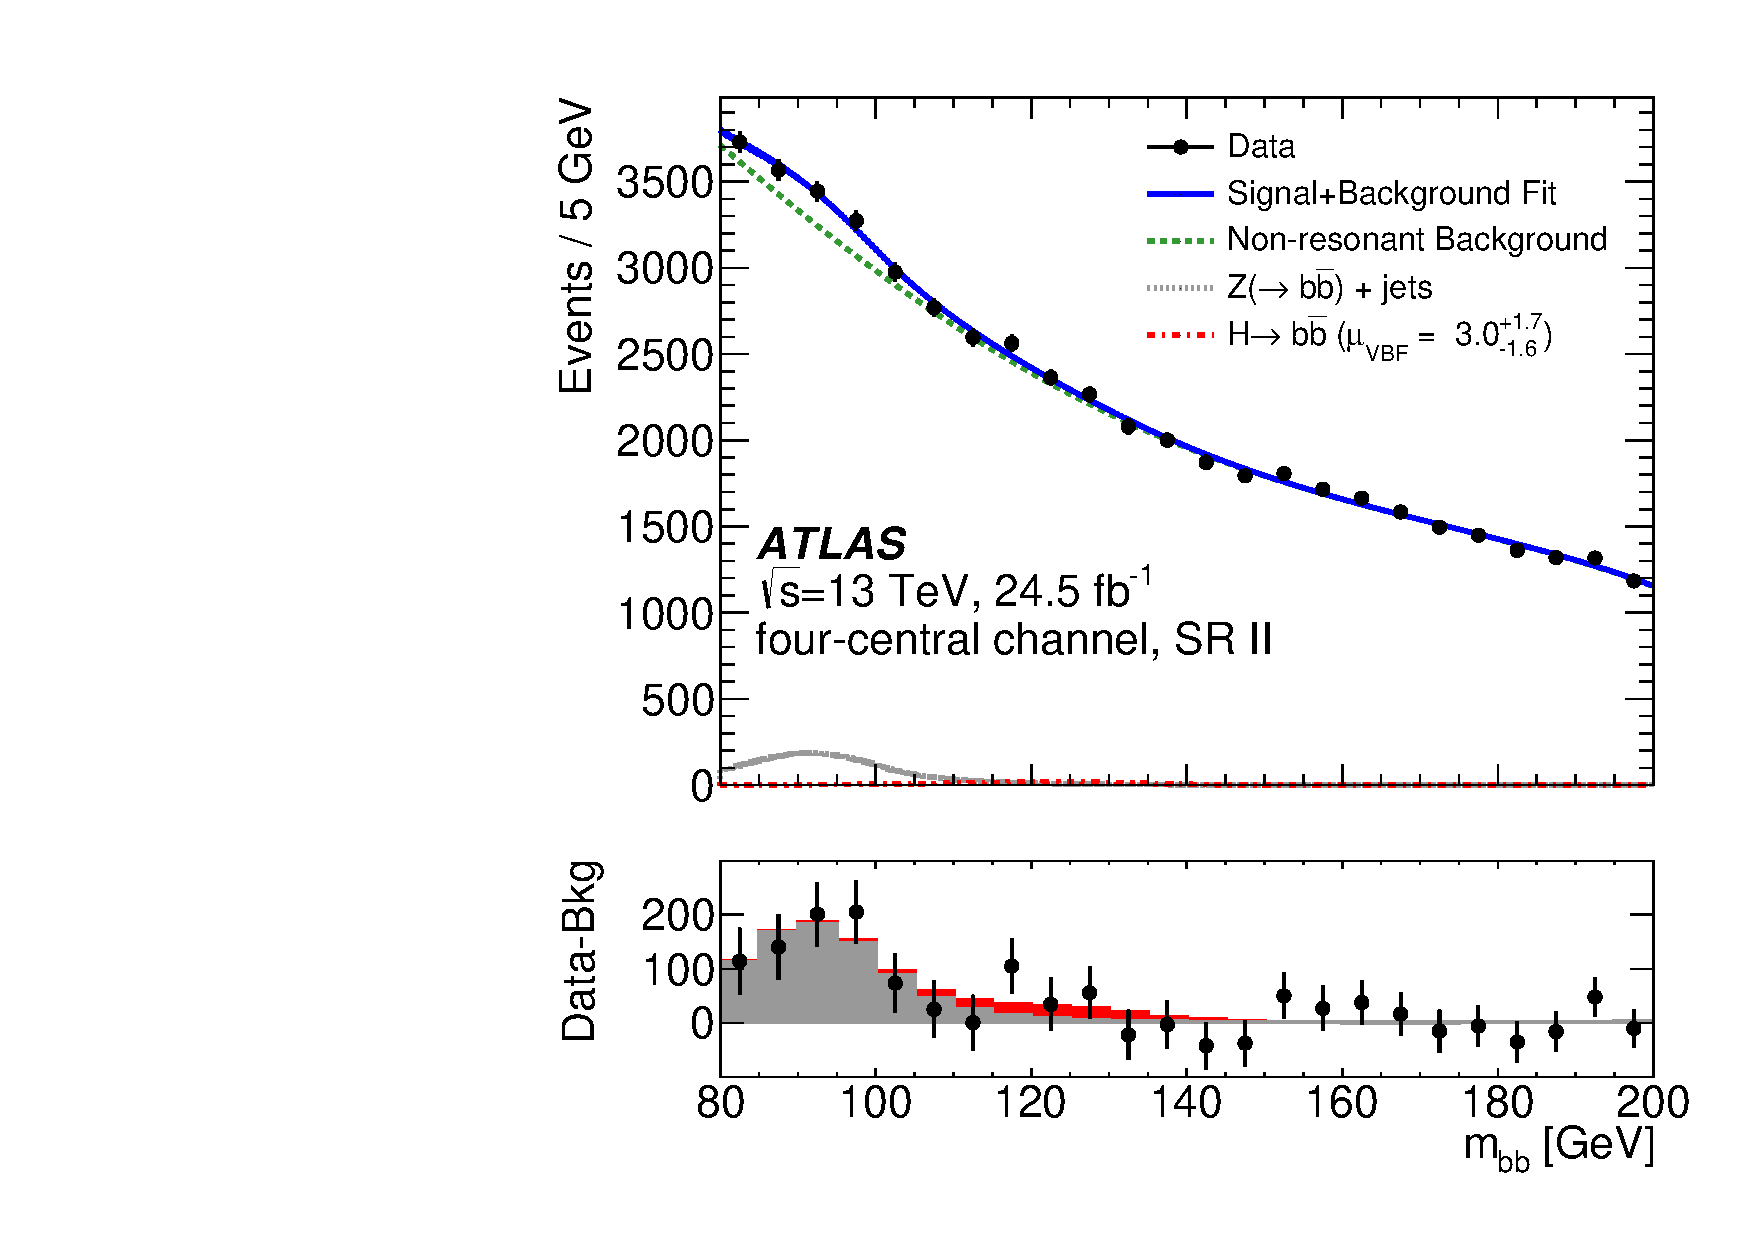
\includegraphics[width=0.48\textwidth]{figures/VBF/comb_vbfonly_testVBF_ICHEP_4cen_SRII_vbfincl.pdf}\\
 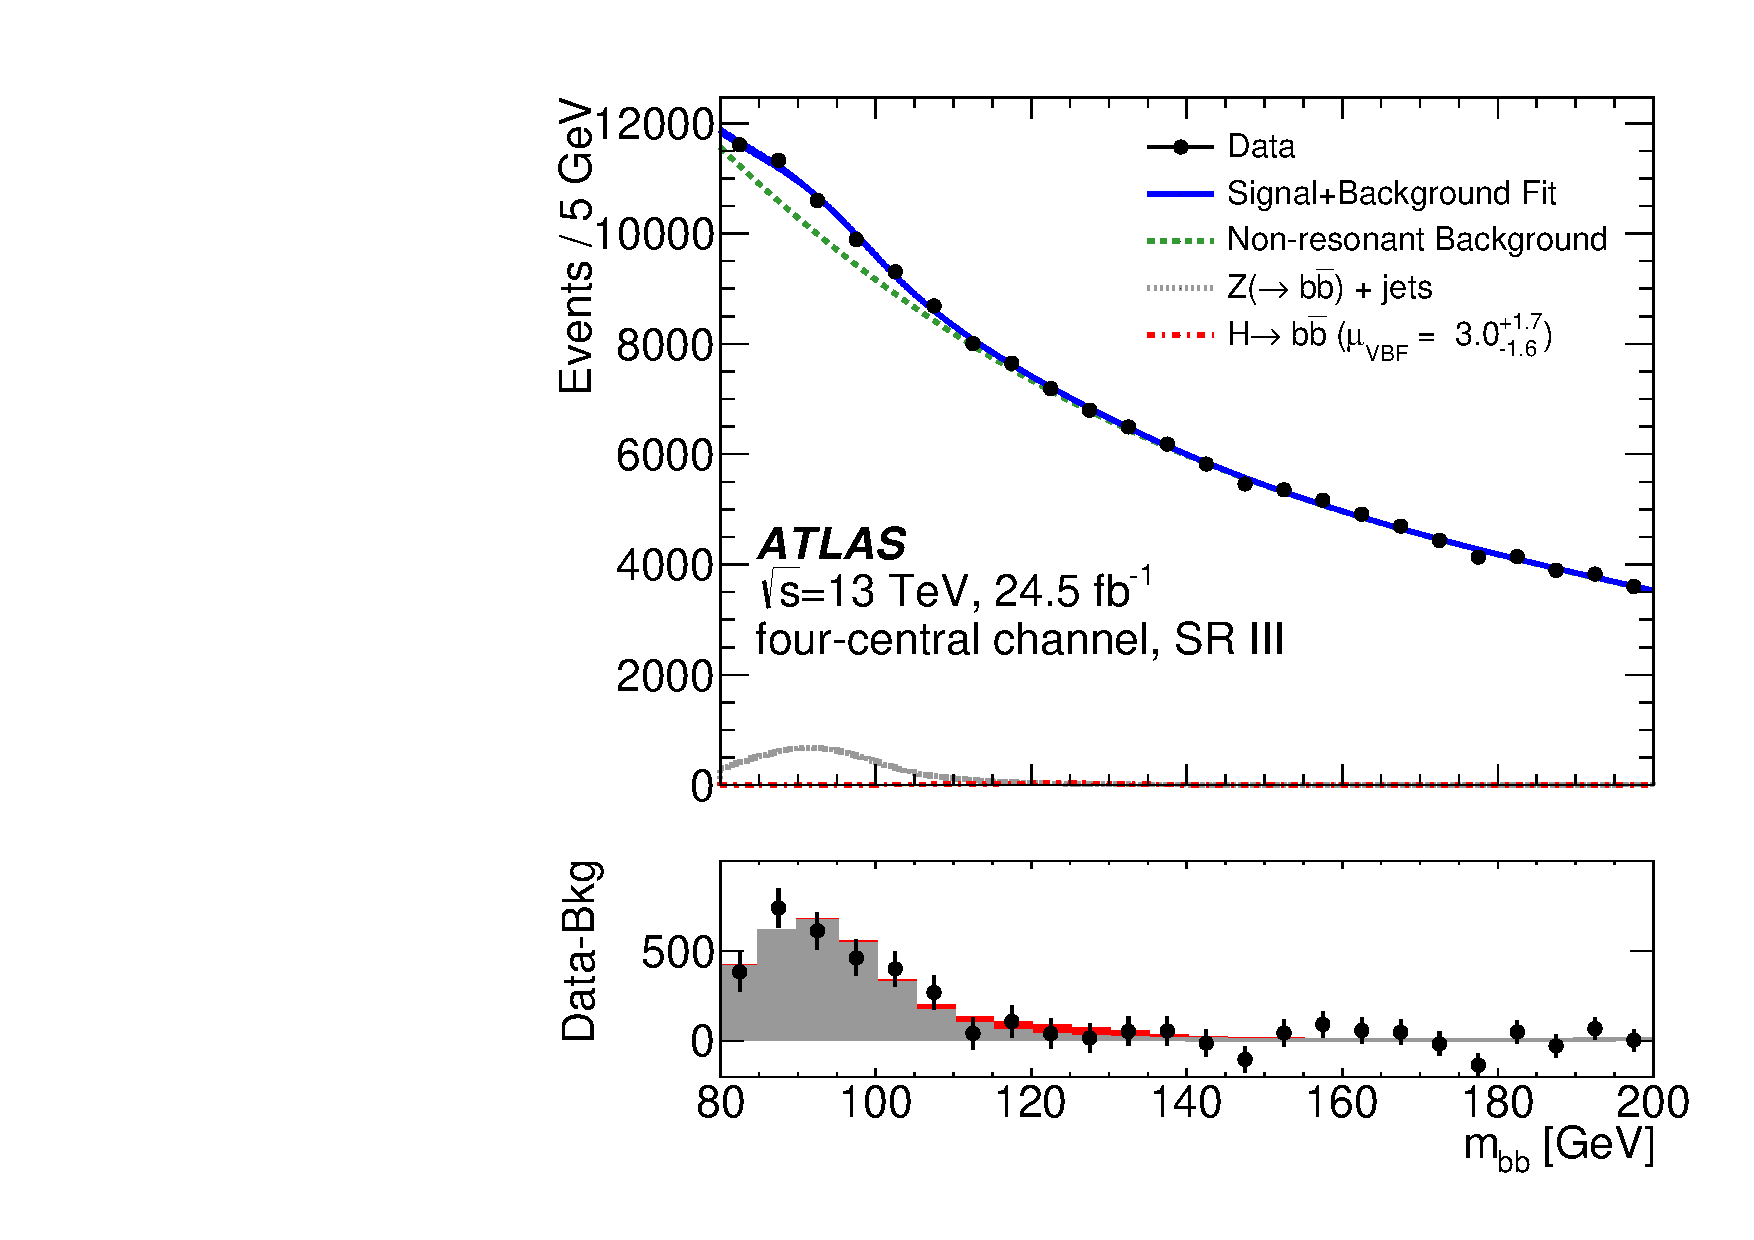
\includegraphics[width=0.48\textwidth]{figures/VBF/comb_vbfonly_testVBF_ICHEP_4cen_SRIII_vbfincl.pdf}
 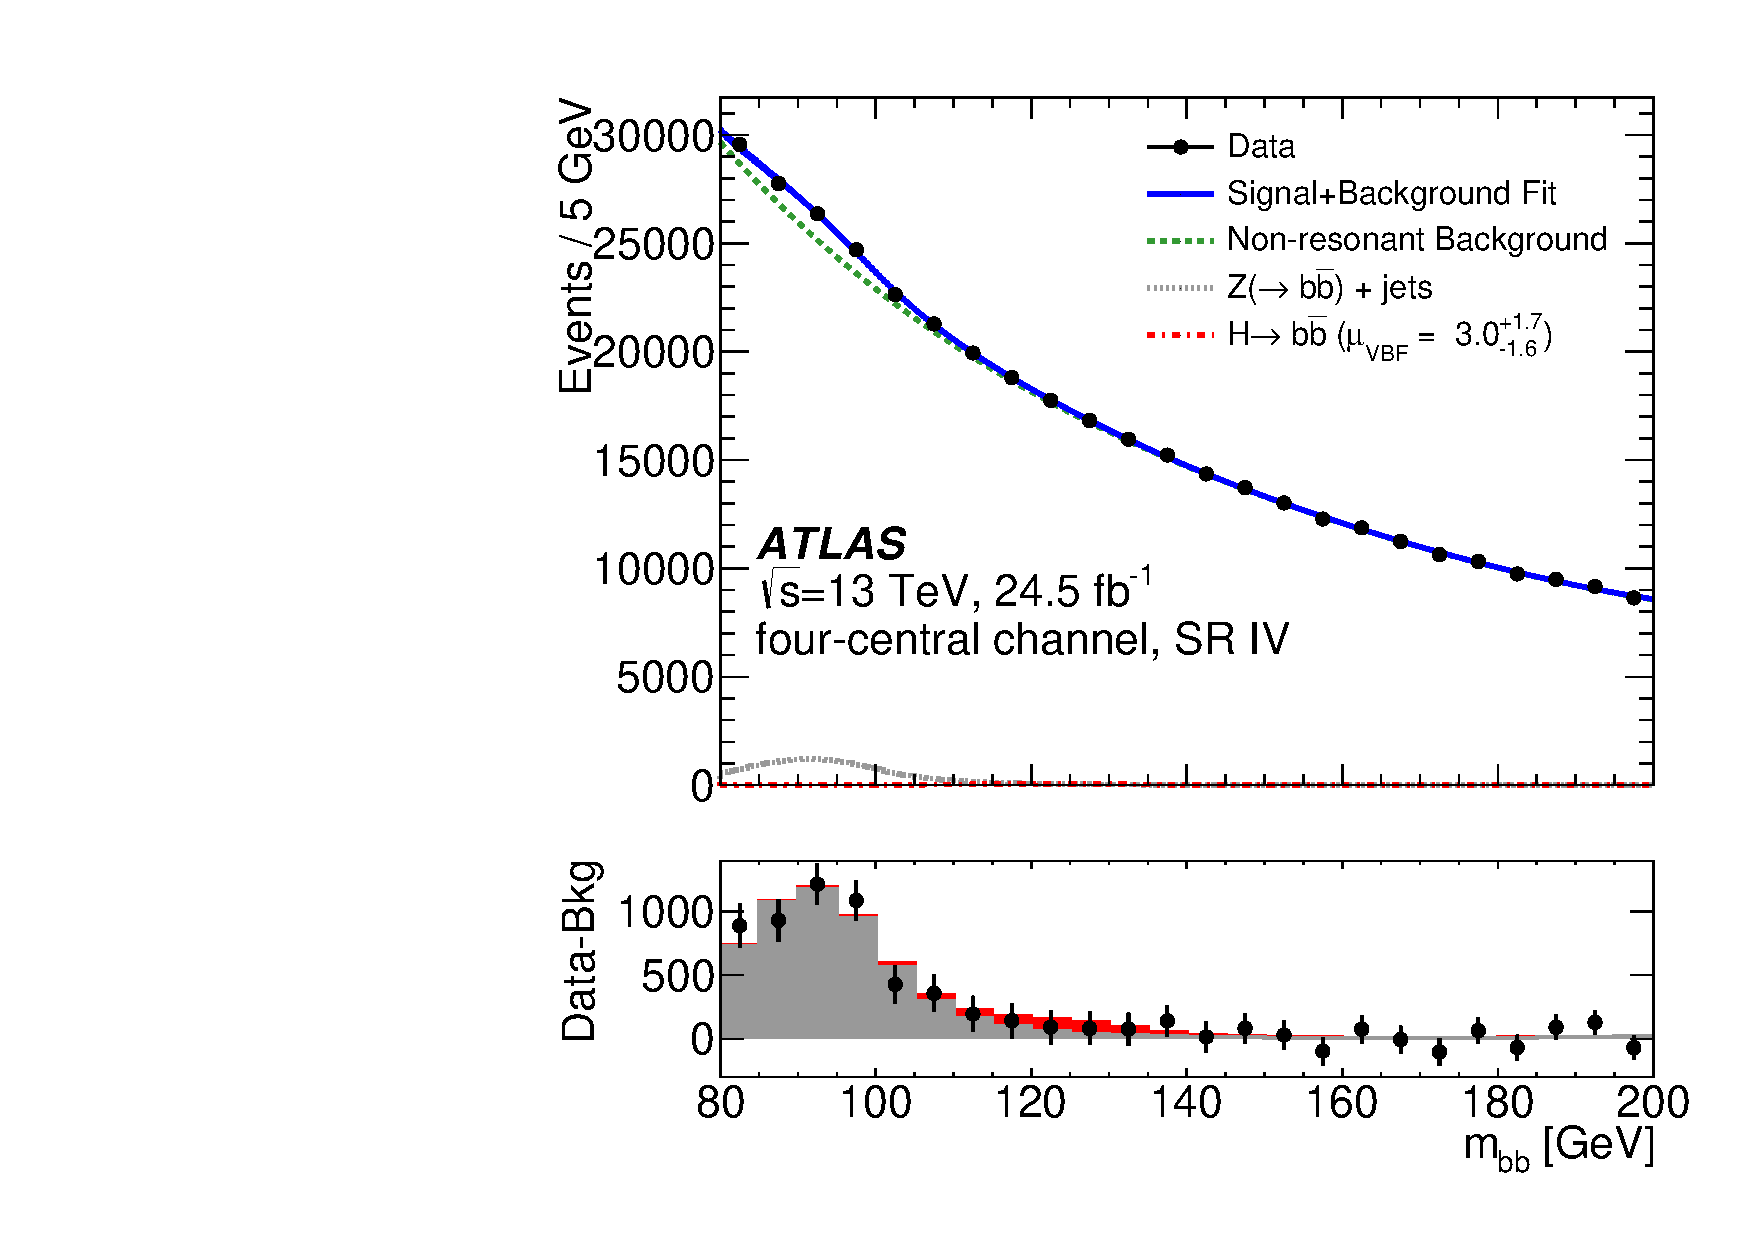
\includegraphics[width=0.48\textwidth]{figures/VBF/comb_vbfonly_testVBF_ICHEP_4cen_SRIV_vbfincl.pdf}\\

\caption{Data and fit model comparison for the combined fit of $\mu_{VBF}$ extraction in the \fourcentral channel}
  \label{fig:higgsfit_4cen}
\end{figure}



\begin{figure}[htbp]
\centering

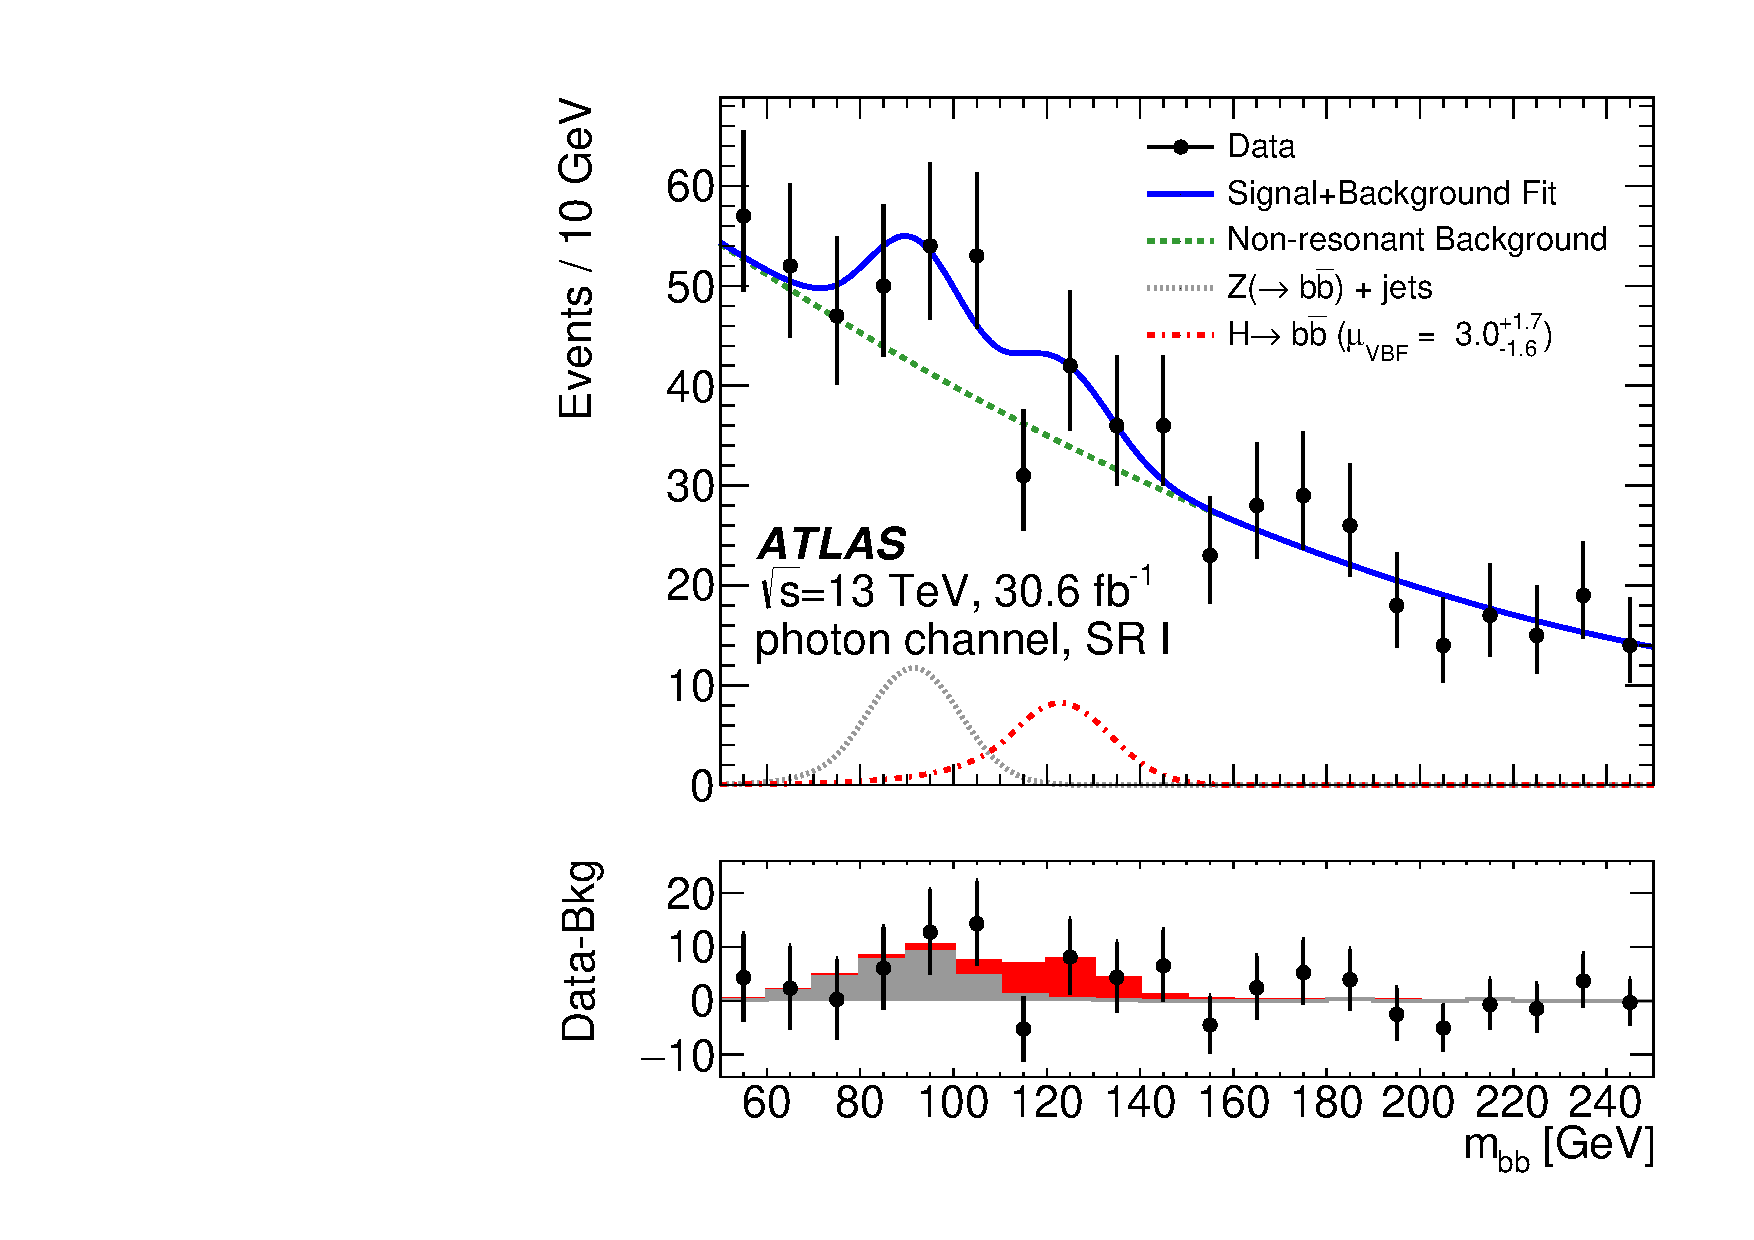
\includegraphics[width=0.48\textwidth]{figures/VBF/comb_vbfonly_testchannel1_vbfg.pdf}
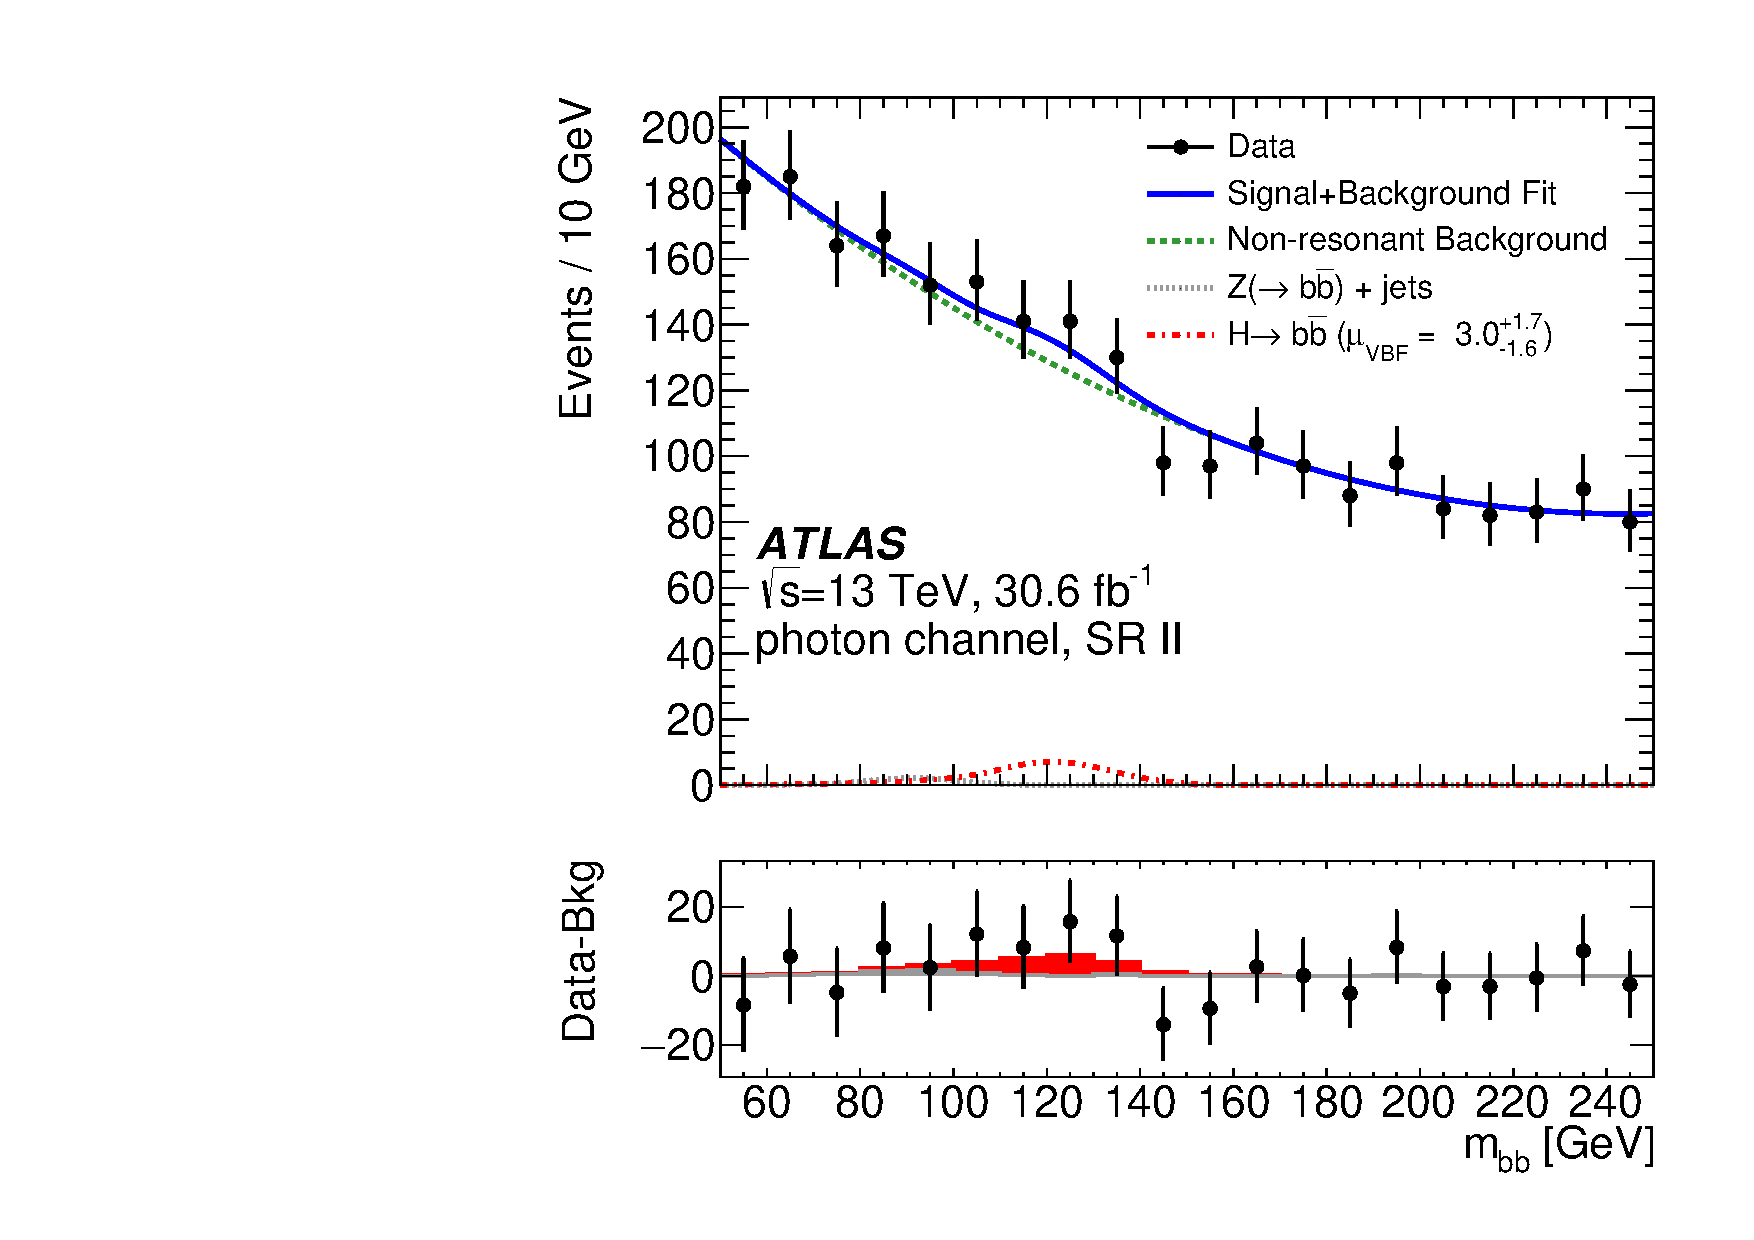
\includegraphics[width=0.48\textwidth]{figures/VBF/comb_vbfonly_testchannel2_vbfg.pdf}
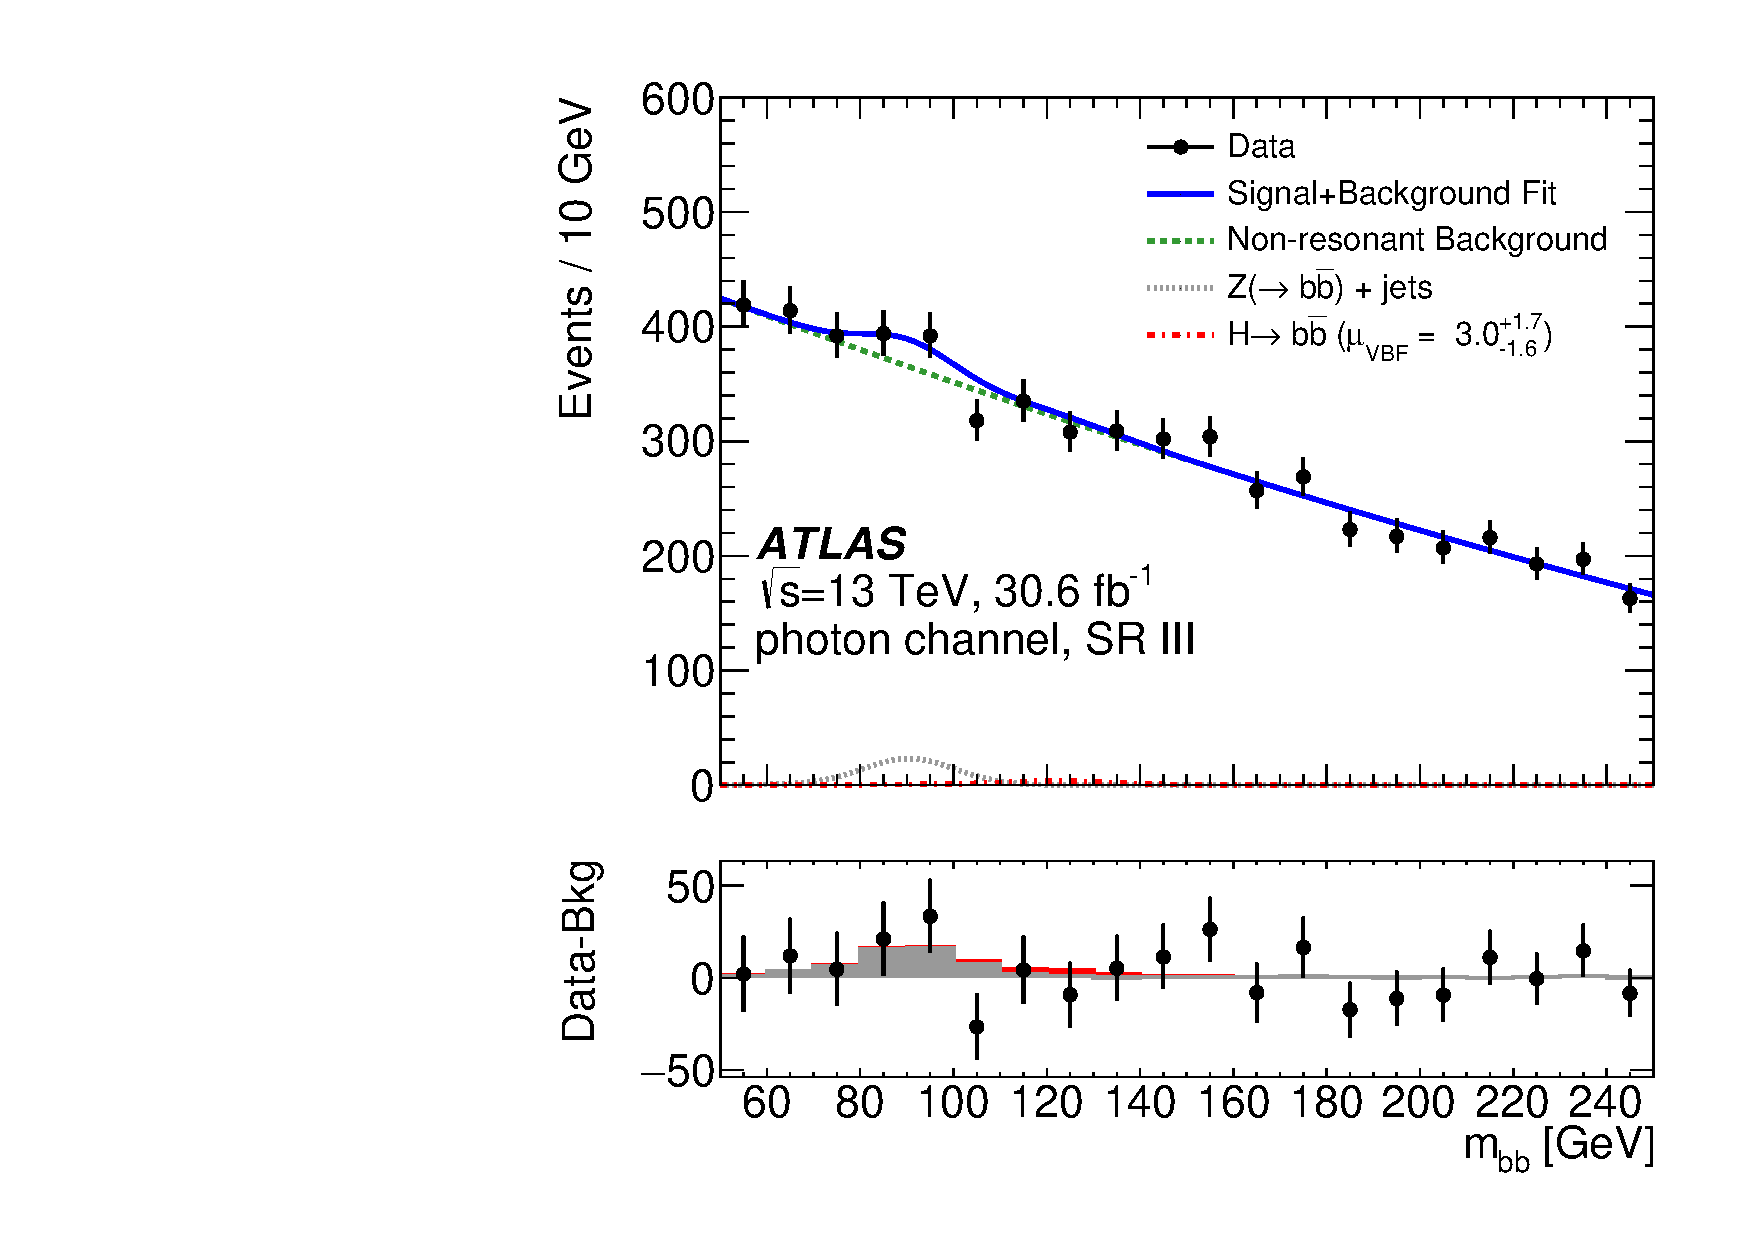
\includegraphics[width=0.48\textwidth]{figures/VBF/comb_vbfonly_testchannel3_vbfg.pdf}
\caption{Data and fit model comparison for the combined fit of $\mu_{VBF}$ extraction in the \textit{photon} channel}
\label{fig:mbb_postfit_photon}
\end{figure}


\begin{figure}[htbp]
  \centering
  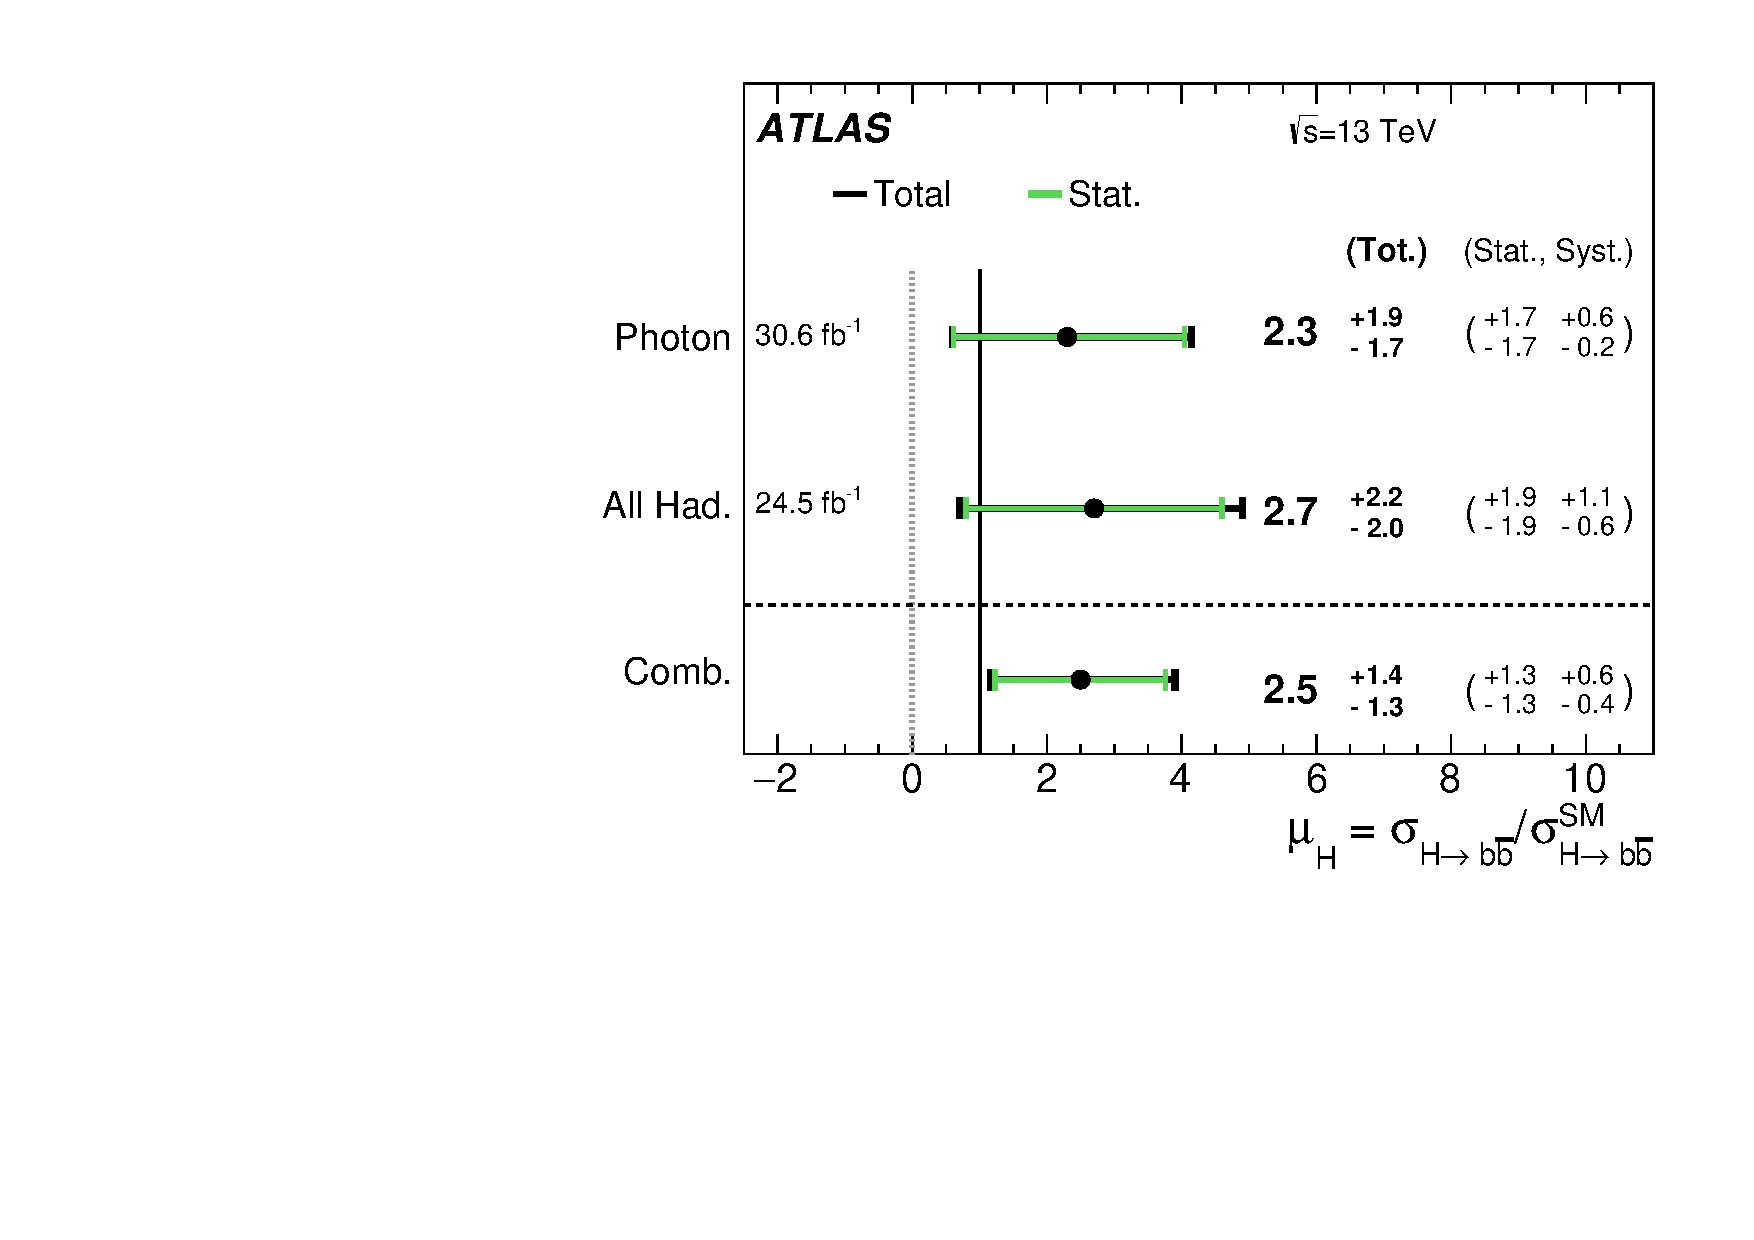
\includegraphics[width=0.49\textwidth]{figures/VBF/Plot_mu_summary_VBF.pdf}
  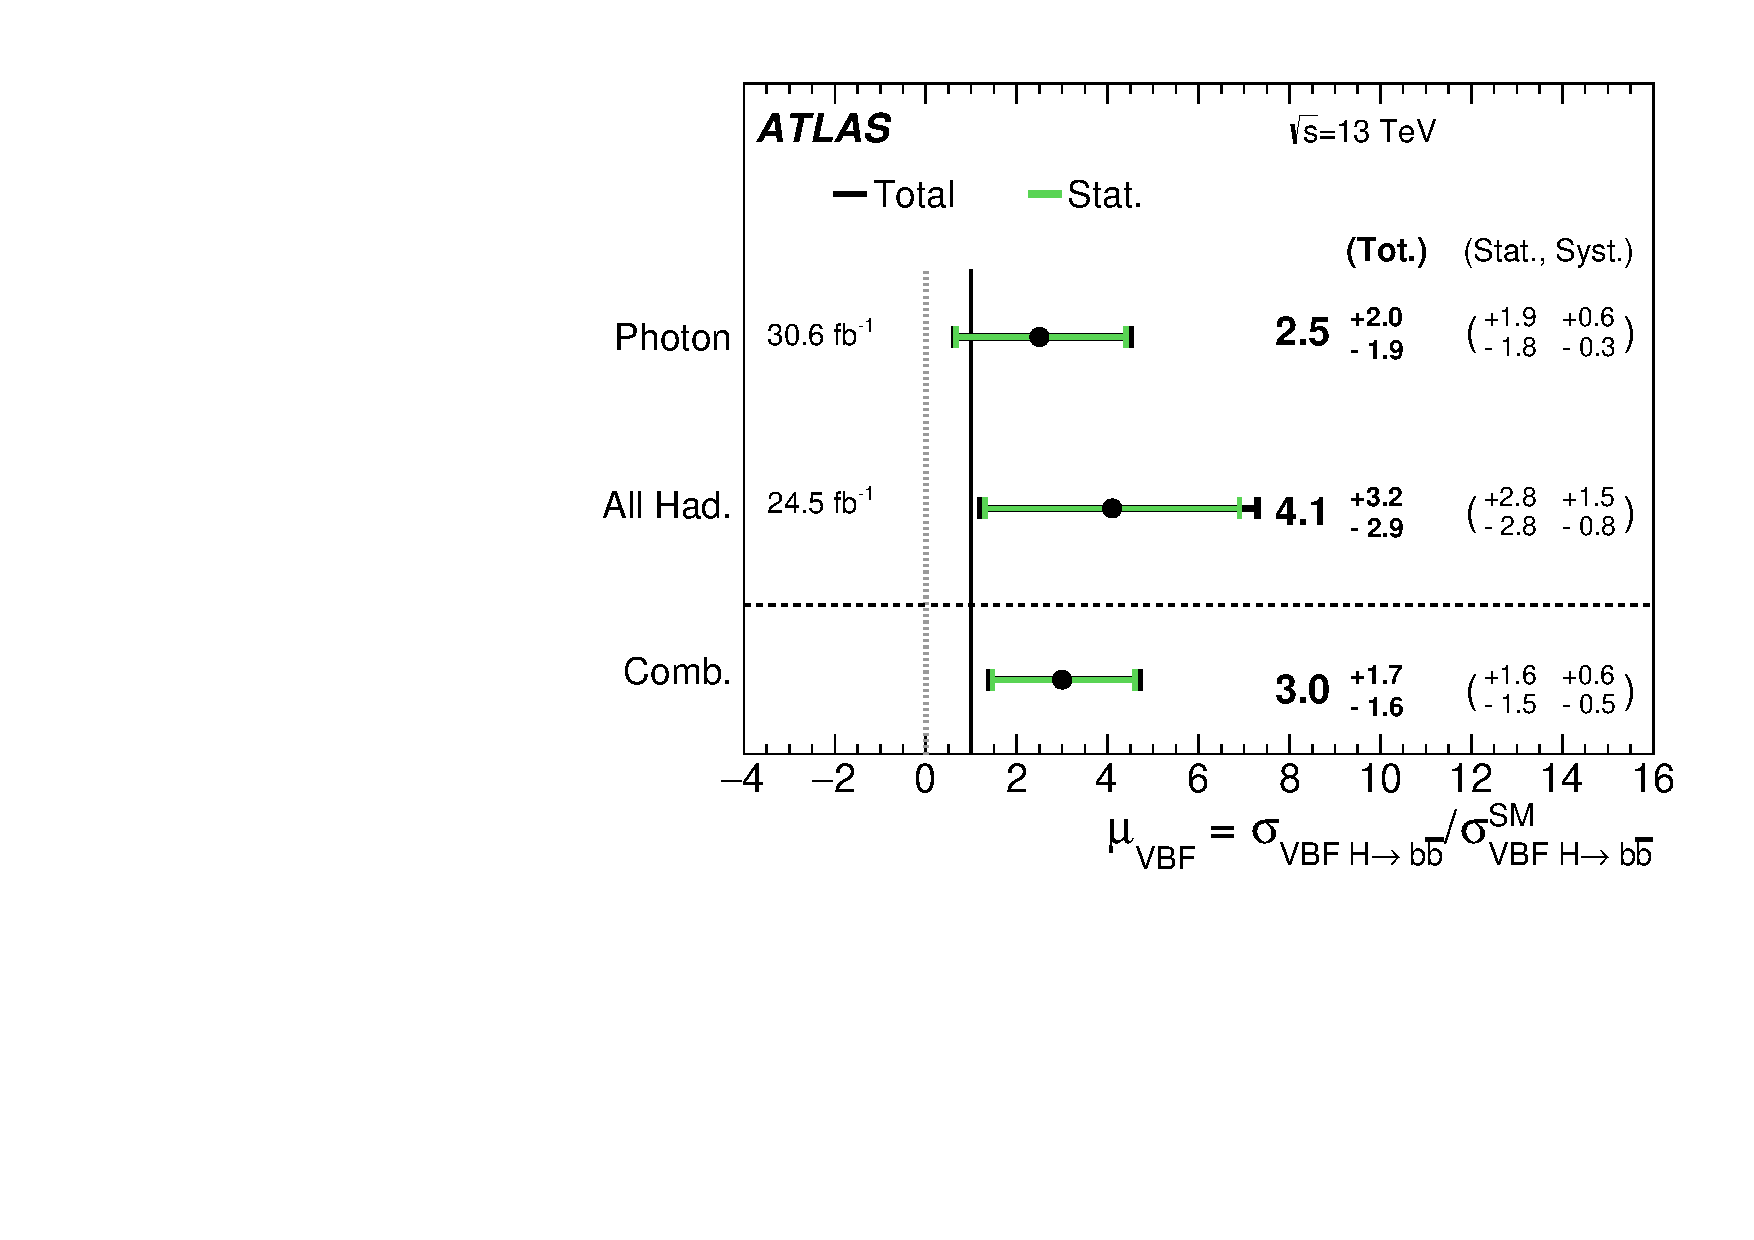
\includegraphics[width=0.49\textwidth]{figures/VBF/Plot_mu_summary_VBFonly.pdf}

\caption{Summary of the extraction of $\mu_{H}$(left) and $\mu_{VBF}$(right) for  \textit{all-hadronic}, \textit{photon} and combination fits.}
  \label{fig:vbf-summary}
\end{figure}



%\begin{figure}[htbp]
%  \centering
% 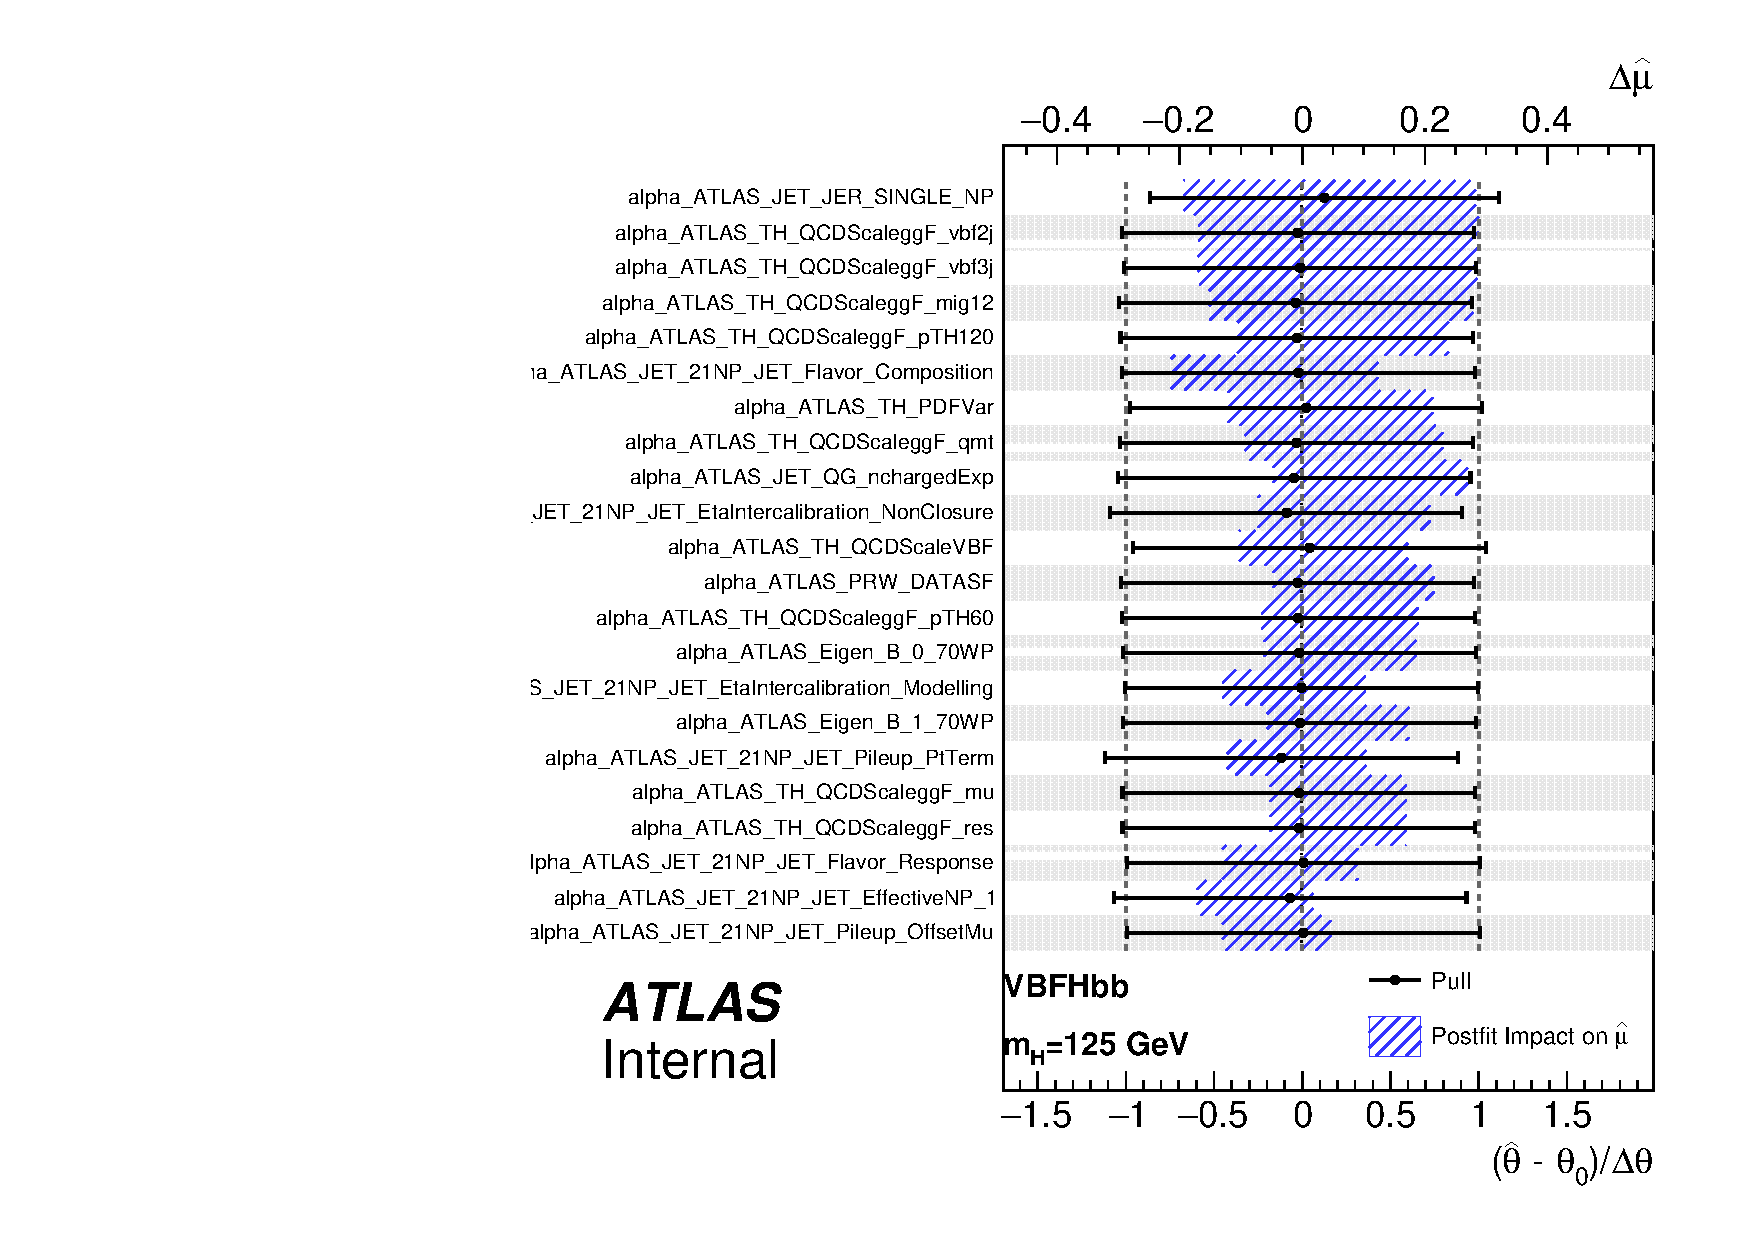
\includegraphics[width=0.8\textwidth]{figures/VBF/VBFHbb_pulls_125.pdf}
% \caption{Nuisance parameter post-fit impact and pulls are plotted for the data fit. Only the constrained NPs are shown. The uncertainties follow the naming defined in Table. \ref{tab:systnames}.}
%  \label{fig:vbf-higgsfitpull}
%\end{figure}

Regarding the treatment of uncertainties, both the inclusive and photon analyses apply systematics trimming. The inclusive analyses ignore nuisance parameters with yield impact $<0.5\%$ while the photon analysis ignore systematics with yield impact $<1\%$. Some NPs, for instance the third effective NP of jet energy scale may pass the systematics trimming cut of one analysis but not the other and therefore only show up in the combination fit for one analysis. 

Same set of nuisance parameters of detector related uncertainties including jet energy scale/resolution, luminosity, pile-up reweighting and q/g tagging is used by both analyses and hence treated as correlated.  $b$-tagging related uncertainties are an exception because the operating points are different between the two analyses. The inclusive analysis uses 70\% and 85\% WPs for \twocentral and \fourcentral channels respectively and the VBF$+\gamma$ analysis uses the 77\% WP. We experimented correlating NPs of the $b$-tagging uncertainties with highest impact, e.g. alpha\_FT\_EFF\_Eigen\_B\_0 of different WPs, across the two analyses and observed negligible change in the final result. Therefore the $b$-tagging NPs are left to be un-correlated.

Common terms of theoretical uncertainties including QCD scale of VBF process, parton shower and variation of $ttH$ yield are also correlated as the underlying variations are derived with same approaches. Background systematics such as non-resonant background normalization/parameterization, Z normalization and spurious signals are specific to each analysis and are not correlated.

The combination fit pull for $\mu_H$ is shown in Fig.\ref{fig:vbf-higgsfitpull_combination}. The combination fit pull for $\mu_{VBF}$ is shown in Fig.\ref{fig:vbf-vbffitpull_combination}. None of the systematics nuisance parameters are pulled significantly from their central values. One event display for the SRI of the \twocentral channel, the most sensitive BDT region, is shown in Fig.\ref{fig:vbf-evtdisplay}.


%%% no longer needed as VBF inclusive breaks down the QCD scale for VBF and ggF separately:  The inclusive and VBF$+\gamma$ analyses have some overlaps in the treatment of the QCD scale uncertainty although do not use exactly the same procedure therefore, by default, it is treated as uncorrelated.  The VBF$+\gamma$ analysis generates samples at truth level with changes by factors of two in the QCD scale and then does a truth-level calculation of the impact on the acceptance and normalization.  This analysis uses weights generated according to the \textit{WG1 scheme} (see Section~\ref{sec:vbf-syst_model}). Since it is a large systematic uncertainty for both analyses, we also try to correlate this particular nuisance parameter. The combined fit correlating the QCD scale uncertainty yields $\mu_H = 2.40^{+1.37}_{-1.32}$, which has a negligible difference with respect to the uncorrelated treatment. Hence we eventually adopt the result treating QCD scale as un-correlated as it is a more conservative approach. 


\begin{figure}[htbp]
  \centering
 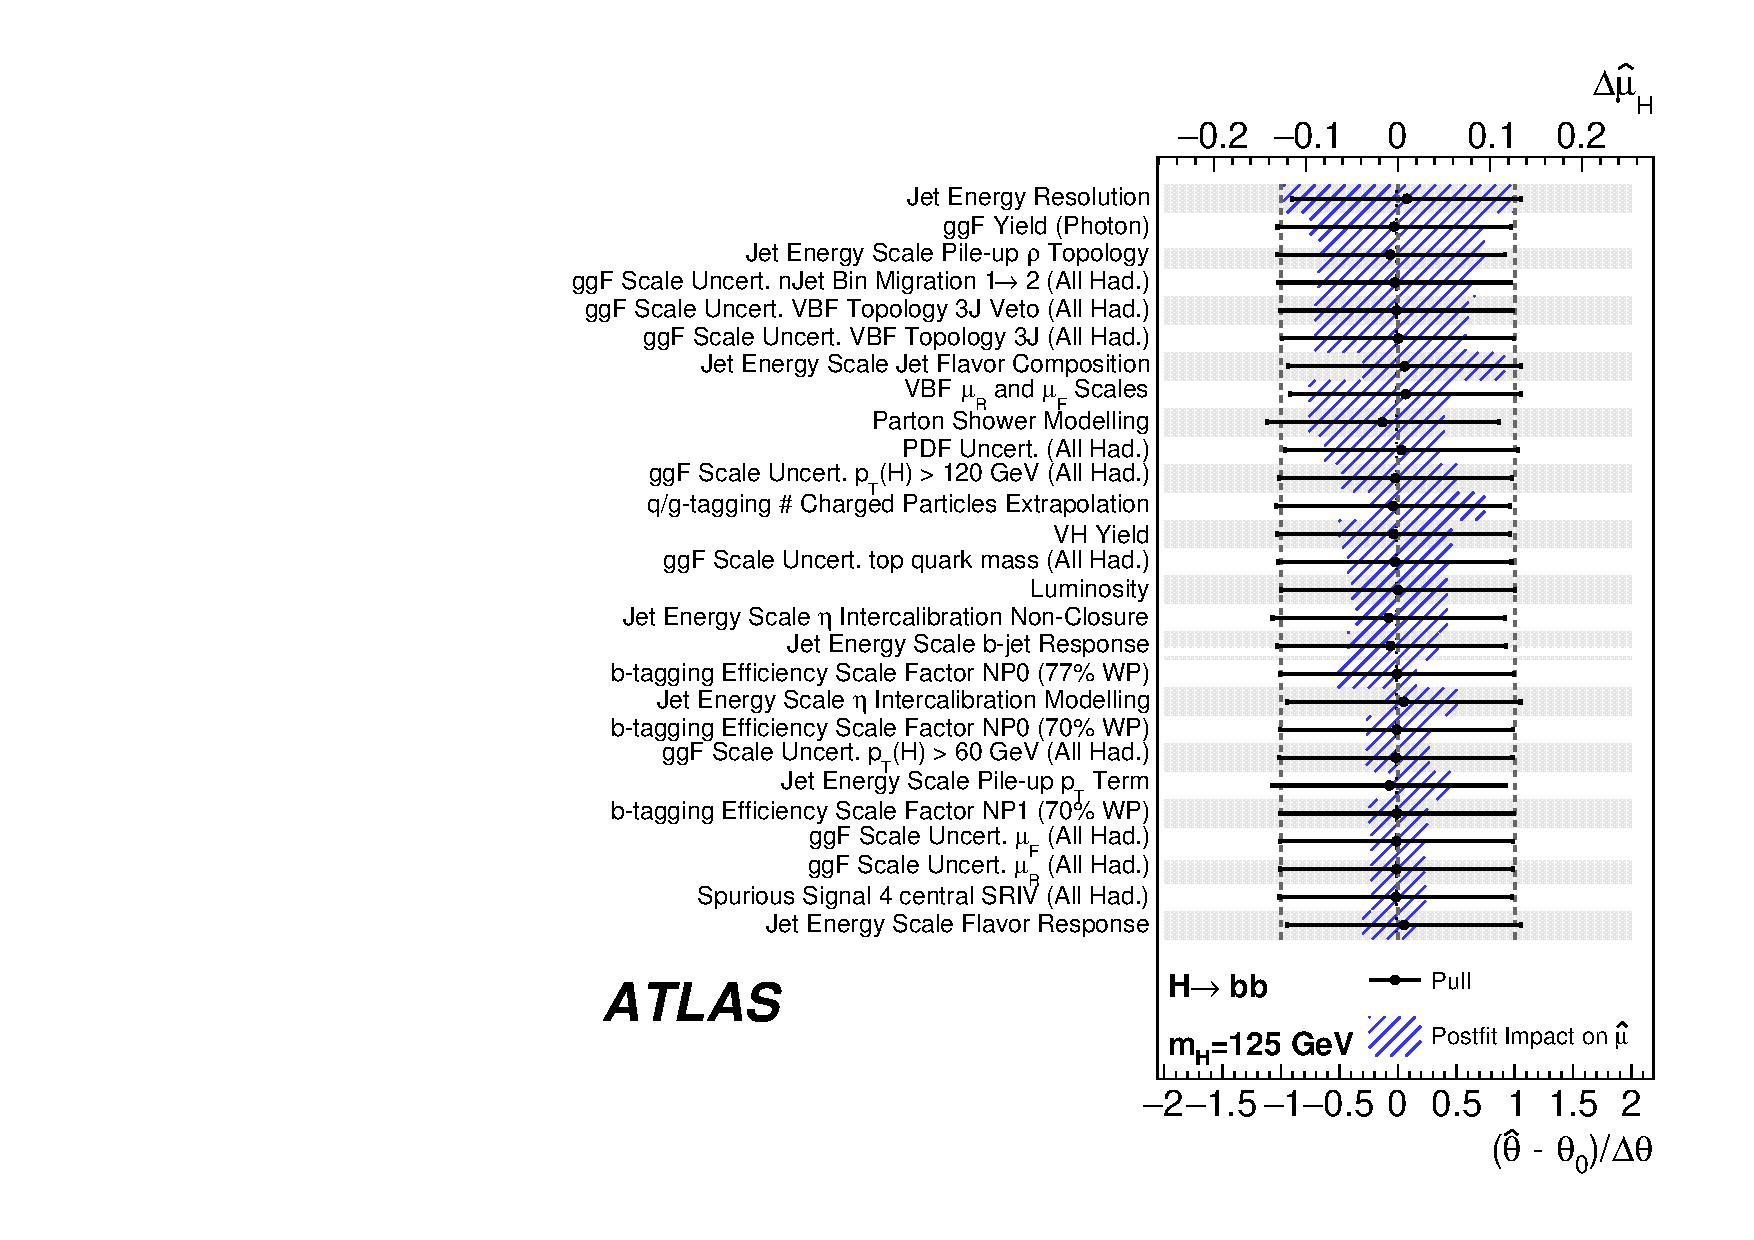
\includegraphics[width=0.8\textwidth]{figures/VBF/VBFHbb_Combined_pulls_125.pdf}
\caption{Data fit pulls for nuisance parameters with a post-fit impact $> 2$ \% for $\mu_H$ combining VBF inclusive and VBF$+\gamma$ analyses.}
  \label{fig:vbf-higgsfitpull_combination}
\end{figure}

\begin{figure}[htbp]
  \centering
 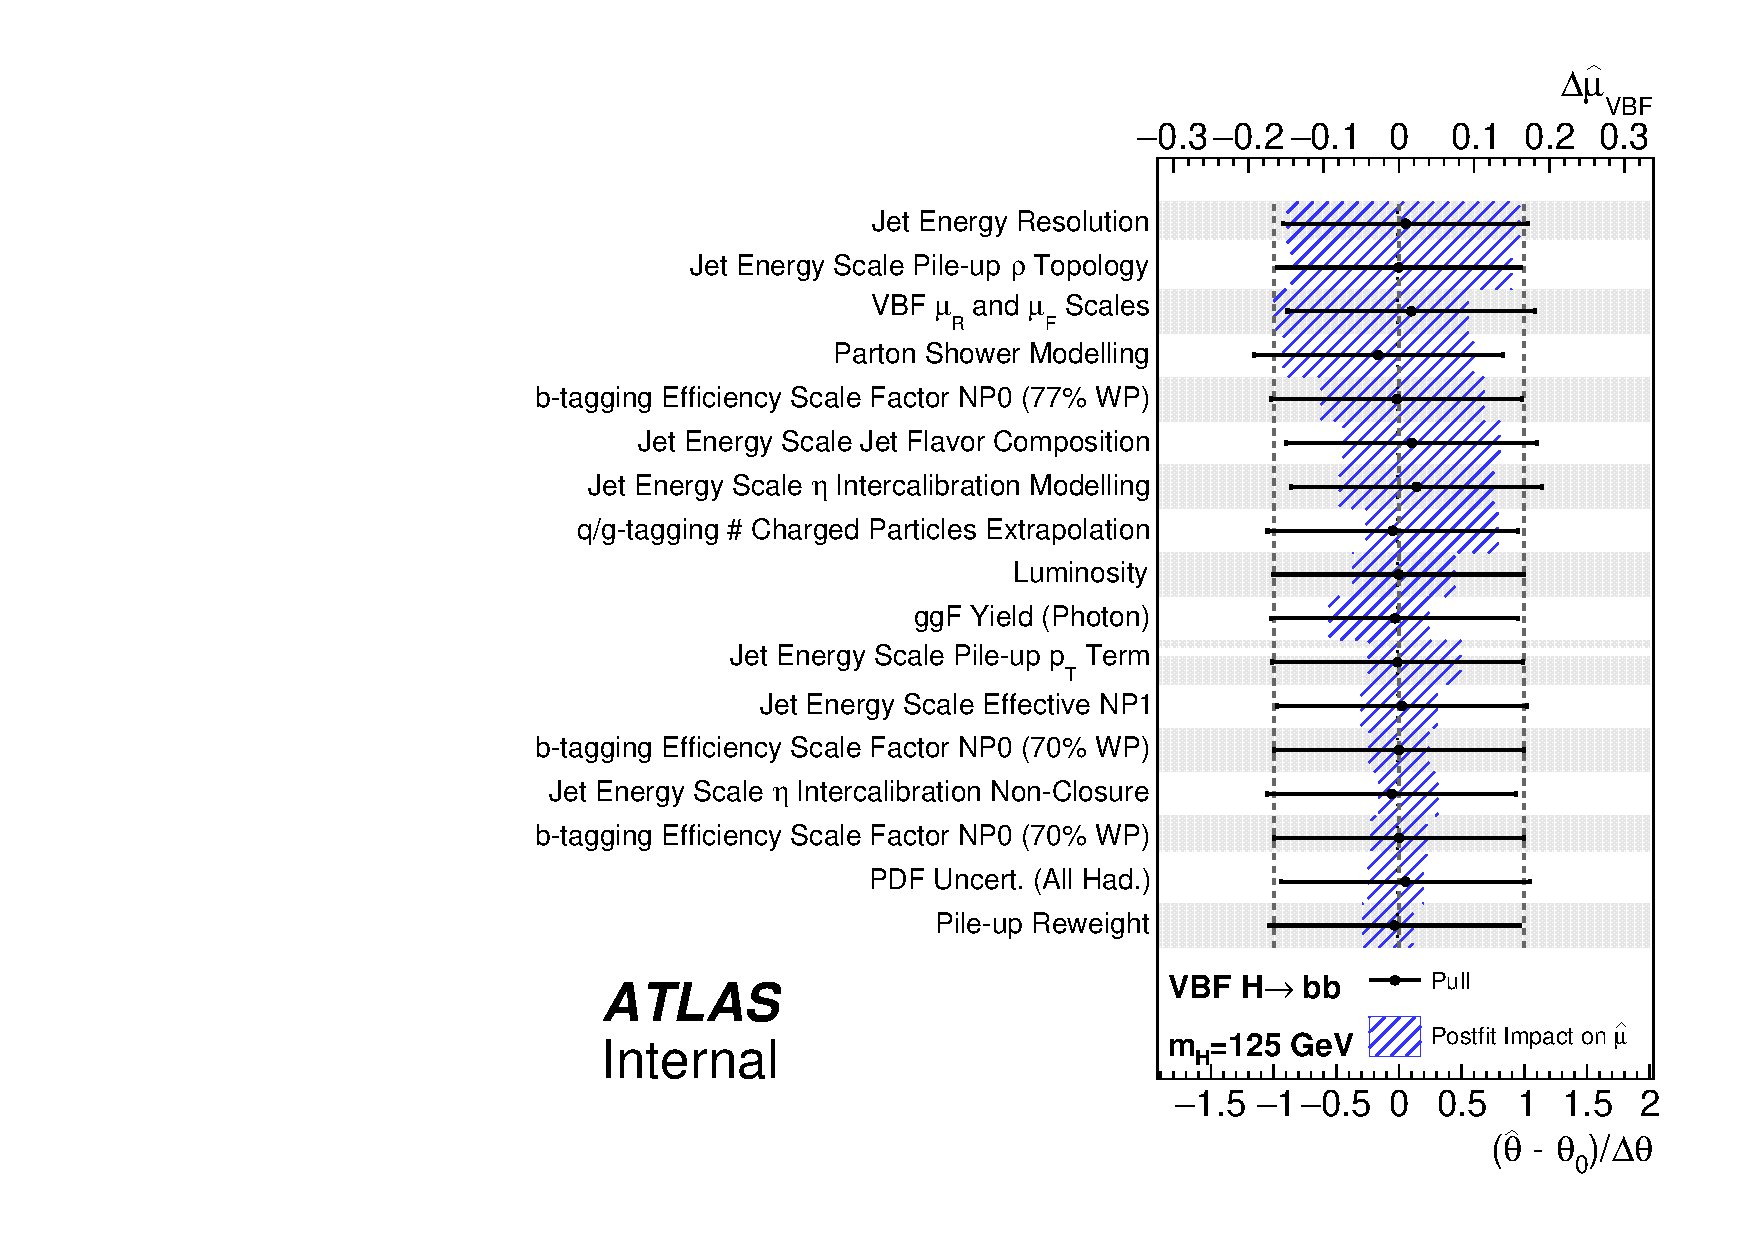
\includegraphics[width=0.8\textwidth]{figures/VBF/VBFHbb_Combined_vbfonly_pulls_125.pdf}
\caption{Data fit pulls for nuisance parameters with a post-fit impact $> 2$ \% for $\mu_{VBF}$ combining VBF inclusive and VBF$+\gamma$ analyses.}
  \label{fig:vbf-vbffitpull_combination}
\end{figure}


\begin{figure}[htbp]
  \centering
 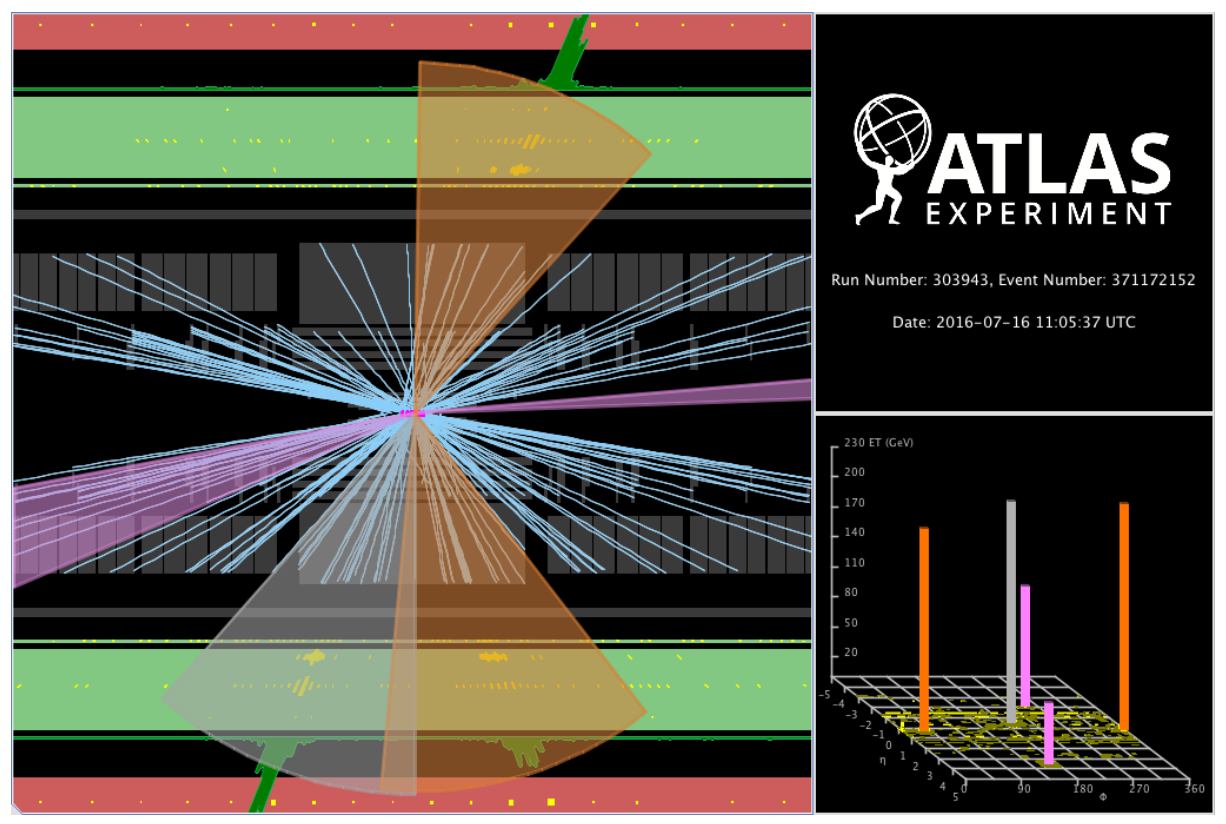
\includegraphics[width=0.8\textwidth]{figures/VBF/EvtDisplay2cen}
\caption{Event display of a \twocentral candidate event in SR I of the with \Mbb = 147 GeV. The cones representing the jets are colored magenta for the forward jets and orange for the b-tagged jets. The transverse momenta of the leading forward jet and sub-leading forward jet are 130.5 GeV and 82.0 GeV respectively. The pseudorapidity of the leading forward jet and sub-leading forward jet are -2.0 and 3.6 respectively}
  \label{fig:vbf-evtdisplay}
\end{figure}



%-------------------------------------------------------------------------------
\section{Conclusions}
\label{sec:conclusion}
%-------------------------------------------------------------------------------
The Run II ATLAS experiment verfied more aspects of the SM. At the same time, there is not much hint of new physics. As the energy of LHC will remain 13-15 \tev for the rest of its lifetime, one way of looking for new physics is to measure SM particles as precisely as possible. The VBF \Hbb mentioned in Chapter \ref{chap:vbf} agreed with Standard Model prediction. However the current sensitivity of this search is low and certainly far from the point that we can perform precise measurement of this combination of Higgs production and decay mode. With the experience of this round of analysis, we have identified a few a aspects to improve the analysis.

A number of analysis specific improvements could be made in the future. Currently, the Higgs sensitivity suffered greatly from the fact that the \zbb contribution normalizations are left to float in the likelihood fit (Sec.\ref{sec:vbf-statanalysis}). Partly also due to a trigger turn-on which cuts into the $Z$ peak, around 80-90 \gev regime, the \zbb contribution is degenerate with the non-resonant background which is also parameterized with floating parameters. If we could reasonably estimate the $Z$ yield and fix its normalization while applying moderate uncertainties, the sensitivity of Higgs would be greatly improved. Potentially one could adopt the same ``embedding'' strategy as used in $h\rightarrow \tau \bar{\tau}$ analysis\cite{HIGG-2013-32}, which takes $h\rightarrow \mu \bar{\mu}$ events from data and replaces the final state $\mu$ with $\tau$. This method models the Higgs production accurately in the VBF corner phase spaces. Another aspect which could be improved is the multivariate analysis. Currently, the non-resonant background in all signal regions are modeled with independent parameters. If the  multi-variate analysis would yield same shapes for all signal regions, then all of them could be modeled with the same set of parameters. Pioneer works such as \cite{ann} has shown that Adversarial Neural Network(ANN) is a great tool for feature invariant classification problem and showed sensitivity improvement of $Z'$ search when applying ANN for large radius jet tagging

Besides, the exploration of a few programs which not only benefit the VBF \Hbb search but could also improve other SM or BSM analyses should continue in the future. The RNN based $b$-tagger which are discussed in Chapter \ref{chap:btagging} if also deployed online can help lower the threshold of $b$-jet triggers and benefit all analyses with final states containing $b$-hadrons. The CNN tagger documented in Chapter \ref{chap:qgtagging} once calibrated and also developed for the forward detector region where track varaibles such as \ntrk are not available can be used to mitigate backgrounds for all VBF Higgs analyses. Analyses such as \cite{Aaboud:2017ecz} and \cite{2h4b}, show that boosted Higgs is a pure phase space for SM and BSM searches. Such study should also be applied to VBF production mode. Jet measurements like the \gbb analysis in Chapter \ref{chap:gbb} could improve the modeling of QCD and may in future make the jet Monte Carlo precise enough for direct QCD background estimation for boosted Higgs searches. 


%-------------------------------------------------------------------------------
\section*{Acknowledgments}
%-------------------------------------------------------------------------------

% From https://twiki.cern.ch/twiki/bin/view/AtlasProtected/PubComAcknowledgement
% Acknowledgements for papers with collision data
% Version 14-Feb-2018

% Standard acknowledgements start here
%----------------------------------------------
We thank CERN for the very successful operation of the LHC, as well as the
support staff from our institutions without whom ATLAS could not be
operated efficiently.

We acknowledge the support of ANPCyT, Argentina; YerPhI, Armenia; ARC, Australia; BMWFW and FWF, Austria; ANAS, Azerbaijan; SSTC, Belarus; CNPq and FAPESP, Brazil; NSERC, NRC and CFI, Canada; CERN; CONICYT, Chile; CAS, MOST and NSFC, China; COLCIENCIAS, Colombia; MSMT CR, MPO CR and VSC CR, Czech Republic; DNRF and DNSRC, Denmark; IN2P3-CNRS, CEA-DRF/IRFU, France; SRNSFG, Georgia; BMBF, HGF, and MPG, Germany; GSRT, Greece; RGC, Hong Kong SAR, China; ISF, I-CORE and Benoziyo Center, Israel; INFN, Italy; MEXT and JSPS, Japan; CNRST, Morocco; NWO, Netherlands; RCN, Norway; MNiSW and NCN, Poland; FCT, Portugal; MNE/IFA, Romania; MES of Russia and NRC KI, Russian Federation; JINR; MESTD, Serbia; MSSR, Slovakia; ARRS and MIZ\v{S}, Slovenia; DST/NRF, South Africa; MINECO, Spain; SRC and Wallenberg Foundation, Sweden; SERI, SNSF and Cantons of Bern and Geneva, Switzerland; MOST, Taiwan; TAEK, Turkey; STFC, United Kingdom; DOE and NSF, United States of America. In addition, individual groups and members have received support from BCKDF, the Canada Council, CANARIE, CRC, Compute Canada, FQRNT, and the Ontario Innovation Trust, Canada; EPLANET, ERC, ERDF, FP7, Horizon 2020 and Marie Sk{\l}odowska-Curie Actions, European Union; Investissements d'Avenir Labex and Idex, ANR, R{\'e}gion Auvergne and Fondation Partager le Savoir, France; DFG and AvH Foundation, Germany; Herakleitos, Thales and Aristeia programmes co-financed by EU-ESF and the Greek NSRF; BSF, GIF and Minerva, Israel; BRF, Norway; CERCA Programme Generalitat de Catalunya, Generalitat Valenciana, Spain; the Royal Society and Leverhulme Trust, United Kingdom.

The crucial computing support from all WLCG partners is acknowledged gratefully, in particular from CERN, the ATLAS Tier-1 facilities at TRIUMF (Canada), NDGF (Denmark, Norway, Sweden), CC-IN2P3 (France), KIT/GridKA (Germany), INFN-CNAF (Italy), NL-T1 (Netherlands), PIC (Spain), ASGC (Taiwan), RAL (UK) and BNL (USA), the Tier-2 facilities worldwide and large non-WLCG resource providers. Major contributors of computing resources are listed in Ref.~\cite{ATL-GEN-PUB-2016-002}.
%----------------------------------------------




%-------------------------------------------------------------------------------
\clearpage
%\appendix
%\part*{Appendix}
%\addcontentsline{toc}{part}{Appendix}
%-------------------------------------------------------------------------------

%-------------------------------------------------------------------------------
% If you use biblatex and either biber or bibtex to process the bibliography
% just say \printbibliography here
\printbibliography
% If you want to use the traditional BibTeX you need to use the syntax below.
%\bibliographystyle{bibtex/bst/atlasBibStyleWoTitle}
%\bibliography{VBFPaper2016,bibtex/bib/ATLAS}
%-------------------------------------------------------------------------------

%-------------------------------------------------------------------------------
% Print the list of contributors to the analysis
% The argument gives the fraction of the text width used for the names
%-------------------------------------------------------------------------------
%\clearpage
%\PrintAtlasContribute{0.30}

%-------------------------------------------------------------------------------
\clearpage
\appendix
\part*{Auxiliary material}
\addcontentsline{toc}{part}{Auxiliary material}
%-------------------------------------------------------------------------------

The following material is intended for use in public presentations and on public web pages.
The material will not be included in the submission to the journal.

At the end of the paper approval procedure, this information will be split into a separate document.
%-- see \texttt{atlas-auxmat.tex}.
\input{content/appendix}

\end{document}
